\documentclass[preprint,12pt,eqsecnum,nofootinbib,amsmath,amssymb]{revtex4}

% Date file was last changed:
\newcommand{\datechange}{3/5/2020}
\newcommand{\datestart}{3/5/2020}

% version
\newcommand\draftverson{v1.0}
\newcommand{\fname}{A\_asymtotic\_notes1.0.tex}
\newcommand{\laurnumber}{\draftverson  ~\today ~\currenttime}
\newcommand{\mydate}{\datechange}

% Person who last changed file:>
\newcommand{\whochange}{Robert Singleton}
%
% Project Name, path, informal author names, title
\newcommand{\projname}{Clog Doc}
\newcommand{\dirname}{Clog/doc/dedx}
\newcommand{\myauthors}{Robert Singleton}
\newcommand{\myrunningtitle}{\fname}
\newcommand{\mytitle}{A-Coefficient Study \# 1}



% printing margins
%
\textwidth=6.5in
\textheight=9.5in

% packages
%
\usepackage{graphicx}  % Include figure files
\usepackage{dcolumn}  % Align table columns on decimal point
\usepackage{bm}             % Bold math: $\bm{\alpha}$
\usepackage{latexsym}  % Several additional symbols
\usepackage{fancyhdr}  % Fancy header package
\usepackage{wrapfig}
\usepackage{comment}
\usepackage{dsfont}
\usepackage{mathtools}
\usepackage{datetime}
%\usepackage{showkeys}% Displays equation and fig names
%\usepackage{hyperref}% Hyperlinked references

% local commands
\newcommand{\overoverline}[1]{ {\overline{\overline{#1}}} }
\newcommand{\EMPTYSET}{\varnothing}
\newcommand{\PROOF}{{\tiny PROOF}}
\newcommand{\ALTPROOF}{{\tiny ALTERNATE PROOF}}
\newcommand{\PAR}{$\blacktriangleright$}
\newcommand{\ENDPF}{$\blacksquare$}
\newcommand{\ENDPROOF}{$\blacksquare$}
%\newcommand{\ENDPF}{\square}
%\newcommand{\ENDPROOF}{$\square$}
\newcommand{\AND}{\wedge}
\newcommand{\OR}{\vee}
\newcommand{\NOT}{\neg}
\newcommand{\EQ}{\equiv}
\newcommand{\IFF}{\leftrightarrow}
\newcommand{\IMP}{\rightarrow}
\newcommand{\T}{{\rm T}}
\newcommand{\F}{{\rm F}}
\newcommand{\LOGEQ}{\sim}
\newcommand{\smDash}{{\rule[1mm]{0.1cm}{0.1mm}}}
\newcommand{\dbar}{{d\hskip-0.12cm \rule[2.2mm]{0.15cm}{0.1mm}}}
\newcommand{\smA}{{\scriptscriptstyle \rm A}}
\newcommand{\smB}{{\rm\scriptscriptstyle B}}
\newcommand{\smN}{{\rm\scriptscriptstyle N}}
\newcommand{\smX}{{\rm\scriptscriptstyle X}}
\newcommand{\bvec}[1]{\mathbf{#1}}
\newcommand{\smP}{{\rm\scriptscriptstyle P}}
\newcommand{\smL}{{\rm\scriptscriptstyle L}}
\newcommand{\smT}{{\rm\scriptscriptstyle T}}
\newcommand{\smC}{{\rm\scriptscriptstyle C}}
\newcommand{\smI}{{\rm\scriptscriptstyle I}}
\newcommand{\smR}{{\rm\scriptscriptstyle R}}
\newcommand{\smS}{{\rm\scriptscriptstyle S}}
\newcommand{\smQ}{{\rm\scriptscriptstyle Q}}
\newcommand{\smD}{{\rm\scriptscriptstyle D}}
\newcommand{\smO}{{\rm\scriptscriptstyle 0}}
\newcommand{\smW}{{\rm\scriptscriptstyle W}}
\newcommand{\smCT}{{\rm\scriptscriptstyle CT}}
\newcommand{\smQM}{{\rm\scriptscriptstyle QM}}
\newcommand{\smRe}{{\rm\scriptscriptstyle Re}}
\newcommand{\smIm}{{\rm\scriptscriptstyle Im}}
\newcommand{\smCL}{{\rm\scriptscriptstyle CL}}
\newcommand{\smBPS}{{\rm\scriptscriptstyle BPS}}
\newcommand{\smE}{{\rm\scriptscriptstyle E}}
\newcommand{\smae}{{\rm\scriptscriptstyle ae}}
\newcommand{\extend}[2]{ {#1}^\smallfrown{\! #2} }
\newcommand{\smTC}{{\rm\scriptstyle TC}}
\newcommand{\calT}{ {\cal T}}
\newcommand{\calA}{{\cal A}}
\newcommand{\mathfrakA}{\mathfrak{A}}
\newcommand{\mathfrakB}{\mathfrak{B}}
\newcommand{\mathfrakS}{\mathfrak{S}}
\newcommand{\smGr}{{\rm\scriptscriptstyle gr}}
\newcommand{\smLT}{{\rm\scriptscriptstyle <}}
\newcommand{\smGT}{{\rm\scriptscriptstyle >}}
\newcommand{\smY}{{\rm\scriptscriptstyle Y}}

% % baselineskip modes
\newcommand{\bodyskip}{\baselineskip 18pt plus 1pt minus 1pt}
\newcommand{\bibskip}{\baselineskip16pt plus 1pt minus 1pt}
\newcommand{\tableofcontentsskip}{\baselineskip 14pt plus 1pt minus 1pt}
\newcommand{\footnoteskip}{\baselineskip 12pt plus 1pt minus 1pt}
\newcommand{\abstractskip}{\baselineskip 13pt plus 1pt minus 1pt}
\newcommand{\titleskip}{\baselineskip 18pt plus 1pt minus 1pt}
\newcommand{\affiliationskip}{\baselineskip 15pt plus 1pt minus 1pt}
\newcommand{\captionskip}{\footnotesize \baselineskip 12pt plus 1pt minus 1pt}
\newcommand{\enumerateskip}{\baselineskip 14pt plus 1pt minus 1pt}
\newcommand{\theoremskip}{\baselineskip 13pt plus 1pt minus 1pt}

% theorem
%
\newtheorem{theorem}{Theorem}
\newtheorem{corollary}[theorem]{Corollary}
\newtheorem{definition}[theorem]{Definition}
\newtheorem{lemma}[theorem]{Lemma}
\newtheorem{proposition}[theorem]{Proposition}
\newtheorem{example}[theorem]{Example}
%\newtheorem{theorem}{Theorem}
%\newtheorem{corollary}{Corollary}
%\newtheorem{definition}{Definition}

\pagestyle{fancy}
\lhead{\laurnumber}
%\lhead{}
\chead{}
\rhead{}
\lfoot{}
\cfoot{\thepage}
\rfoot{}

%%
%% begin: draw box
%%
%%%%%%%%%%%%%%%%%%%%%%%%%%%%%%
%%
%%  This macro draws a box around around text, taken 
%%  from ``TeX by Example'', by Arvind Borde p76.
%%
%%   To use: 
%%
%%   \vskip0.3cm
%%   \frame{.1}{2}{16.2cm}{\noindent
%%   \begin{eqnarray}
%%     a = b
%%   \end{eqnarray}
%%   }
%%   \vskip0.2cm
%%
%%%%%%%%%%%%%%%%%%%%%%%%%%%%%%%
%%
\def\frame#1#2#3#4{\vbox{\hrule height #1pt    % TOP RULE
  \hbox{\vrule width #1pt\kern #2pt                     % RULE/SPACE ON LEFT
  \vbox{\kern #2pt                                               % TOP SPACE
  \vbox{\hsize #3\noindent #4}                            % BOXED MATERIAL
  \kern #2pt}                                                        % BOTTOM SPACE
  \kern #2pt\vrule width #1pt}                              % RULE/SPACE ON RIGHT
  \hrule height0pt depth #1pt}                            % BOTTOM RULE
}
%%
\def\myframe#1{\vbox{\hrule height 0.1pt    % TOP RULE
  \hbox{\vrule width 0.1pt\kern 2pt                     % RULE/SPACE ON LEFT
  \vbox{\kern 2pt                                               % TOP SPACE
  \vbox{\hsize 16.5cm\noindent #1}                            % BOXED MATERIAL
  \kern 2pt}                                                        % BOTTOM SPACE
  \kern 2pt\vrule width 0.1pt}                              % RULE/SPACE ON RIGHT
  \hrule height0pt depth 0.1pt}                            % BOTTOM RULE
}
%%
%% draws two boxes around text (use sparingly)
%%
\def\fitframe #1#2#3{\vbox{\hrule height#1pt  % TOP RULE
  \hbox{\vrule width#1pt\kern #2pt             % RULE/SPACE ON LEFT
  \vbox{\kern #2pt\hbox{#3}\kern #2pt}         % TOP,MATERIAL,BOT
  \kern #2pt\vrule width#1pt}                  % RULE/SPACE ON RIGHT
  \hrule height0pt depth#1pt}                  % BOTTOM RULE
}
%%
%% draws a box with shadow around text
%%
\def\shframe #1#2#3#4{\vbox{\hrule height 0pt % NO TOP SHADOW
 \hbox{\vrule width #1pt\kern 0pt             % LEFT SHADOW
 \vbox{\kern-#1pt\frame{.3}{#2}{#3}{#4}       % START SHADOW
 \kern-.3pt}                                  % MOVE UP RULE
 \kern-#2pt\vrule width 0pt}                  % STOP SHADOW
 \hrule height #1pt}                          % BOTTOM SHADOW
}
%%
%%
%% end: draw box
%%
%%  To install as a package on a local host.
%%   a. Append the header ``\usepackage{myboxes}'' to the above macro. Name 
%%   the macreo file myboxes.sty.  Move myboxes.sty into $HOME/texmf/tex/mypackages/. 
%%   You might need to type texhash.
%%   b. T use the package write \usepackage{myboxes} in the preamble.

%
\begin{document}

%% notes info page
%\hfill{\laurnumber}
%\vskip0.3cm
\centerline{{ \Large\bf \projname: \fname}}
\vskip0.25cm 
\centerline{\bf \mytitle}
\vskip0.25cm
\centerline{\myauthors}
\vskip0.75cm 
\baselineskip 14pt plus 1pt minus 1pt
\begin{flushright}
Research Notes   \\[3pt]
{\it Project}:          \\
\projname                      \\
  {\it Path of TeX Source}:          \\
\dirname/\fname                      \\[3pt]
{\it Last Modified By}:            \\
\whochange                         \\
\datechange                        \\[3pt]
{\it Date Started:}                \\
\datestart                         \\[3pt]
{\it Date:}                \\
\draftverson~ \today ~\currenttime \\
\end{flushright}

\baselineskip 20pt plus 1pt minus 1pt

%% mini abstract
%\abstractskip
%\noindent
%These are notes on Logic from Ref.~\cite{ref_chang}.  
%\bodyskip

%% title page
\vskip2.0cm
%\pagebreak
\preprint{\laurnumber}

% publication title page
\title{\titleskip
  \mytitle
}

\author{Robert L Singleton Jr}

\affiliation{\affiliationskip
   School of Mathematics\\
   University of Leeds\\
   LS2 9JT
}

\date{\datechange}

\begin{abstract}
\abstractskip
\vskip0.3cm 
\noindent
This is a study of the asymptotic behavior of the ${\cal
  A}$-coefficients from \verb+Clog/acoeff.f90+.
Each figure is constructed by a Fortran driver \verb+grXXX.f90+ and a
corresponding plotting routine \verb+grXXX.sm+. The plasma under
consideration is equimolar DT with electron number density $n_e$,
electron temperature $T_e$, and ion temperature $T_\smI$. The code
used to generate the data has now been fully checked.

\end{abstract}

%%
\maketitle
%%

% to change page settings
%\thispagestyle{empty}
%\pagestyle{empty}
%\setcounter{page}{0}

\pagebreak
\tableofcontentsskip
\tableofcontents
%\thispagestyle{empty}

%\pagebreak
\newpage
\bodyskip
%\setcounter{page}{1}

\pagebreak
\clearpage

\newpage

\section{A-Coefficients as a Function of Energy}

The {\cal A}-coefficients take the form
%%
\begin{eqnarray}
  {\cal A}_b 
  &=&  
  {\cal A}^\smC_b + {\cal A}^{\Delta Q}_b 
  ~~~\text{where}~~
  {\cal A}^\smC_b 
  =
  {\cal A}^\smC_{b,\smS} +  {\cal A}^\smLT_{b,\smR} \ ,
\label{all}
\end{eqnarray}
%%
with
%%
\begin{eqnarray}
  {\cal A}^\smC_{b,\smS}
  &=& 
  \frac{e_p^2\,\kappa^2_b}{4\pi} \,   
  \left( \frac{\beta_b m_b}{2\pi} \right)^{1/2}\!\!
  v_p\int_0^1 du \, u^{1/2} \,\exp\left\{ - \frac{1}{2} \,
  \beta_b m_b v^2_p \, u \right\}
\nonumber\\
  && \qquad
  \left[ -\ln \left(\beta_b  \frac{e_p e_b}{4\pi} \,
  K \, \frac{m_b}{m_{pb}} \, \frac{u}{1-u} \right) 
  - 2 \gamma + 2 \right] 
\label{wonderclassic}
\\[10pt]
  {\cal A}^\smLT_{b,\smR}
  &=&
  \frac{e_p^2}{4 \pi}\, \frac{i}{2 \pi}
  \int_{-1}^1 \! d\cos\theta\, \cos\theta\,
  \frac{\rho_b(v_p\cos\theta)}
  {\rho_{\rm total}(v_p\cos\theta)}\,F(v_p \cos\theta) 
  \ln\!\left\{\frac{F(v_p\cos\theta)}{K^2}\right\} \,, 
\label{nun}
\\[10pt]
  {\cal A}^{\Delta Q}_b
  &=&
  -\frac{e_p^2\, \kappa_b^2}{4 \pi}\,
  \left( \frac{\beta_b m_b}{2\pi} \right)^{1/2}\,
  \frac{1}{2}\int_0^\infty dv_{pb}
  \bigg\{ 2\, {\rm Re} \, \psi \left( 1 + i \eta_{pb}
  \right) - \ln \eta^2_{pb}  \bigg\}
\nonumber\\
  &&
  \frac{1}{\beta_b m_b v_p v_{pb}} \, 
  \Bigg[ \exp\left\{ - \frac{1}{2}\, \beta_b
  m_b \left( v_p - v_{pb} \right)^2\right\} 
   \left( 1 - \frac{1}{\beta_b m_b v_p v_{pb} } \right) 
\nonumber\\
  && \qquad\qquad\quad
  + \exp\left\{ - \frac{1}{2} \beta_b m_b \left( v_p + v_{pb} 
  \right)^2\right\} 
   \left( 1 + \frac{1}{\beta_b m_b v_p v_{pb} } \right) 
\Bigg]	\,,
\label{regb}
\end{eqnarray}
%% 
and $\eta_{ab}=e_a e_b/4\pi\hbar v_{ab}$.
Figures~\ref{fig:gr001}--\ref{fig:gr003} show the ${\cal A
}$-coefficients for (i) $T_e = T_\smI=10\,{\rm keV}$, (ii) $T_e =
10\,{\rm keV}$ and $T_\smI=100\,{\rm keV}$, and (iii) $T_e=100\,{\rm
  keV}$ and $T_\smI=10\,{\rm keV}$ respectively, all with an electron
number density $n_e=10^{25}\,{\rm cm^{-3}}$.


%%
\vskip-2.5cm 
\begin{figure}[h!]
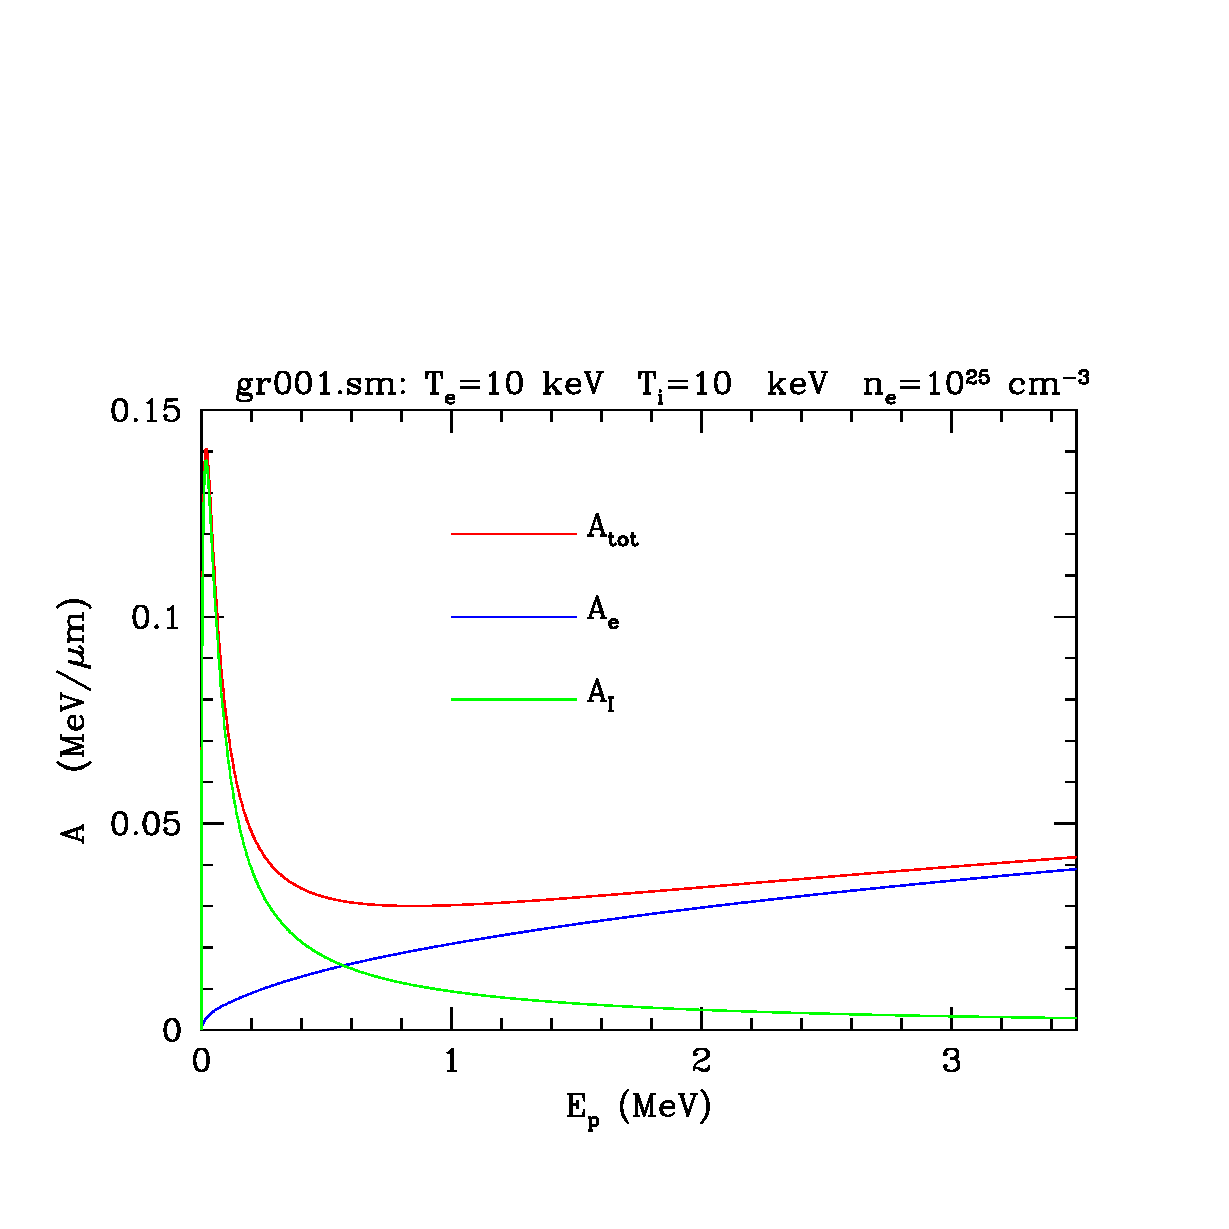
\includegraphics[scale=0.45]{gr001.eps} 
\vskip-0.8cm 
\caption{\footnoteskip  
%%
  Electron and ion components: $n_e=10^{25}\,{\rm cm^{-3}}$,
  $T_e=10\,{\rm keV}$, $T_\smI=10\,{\rm keV}$. [gr001.f90, gr001.sm,
  gr001.dat, gr001.eps]
%%
}
\label{fig:gr001}
\end{figure}
%%

%%
\vskip-2cm 
\begin{figure}[h!]
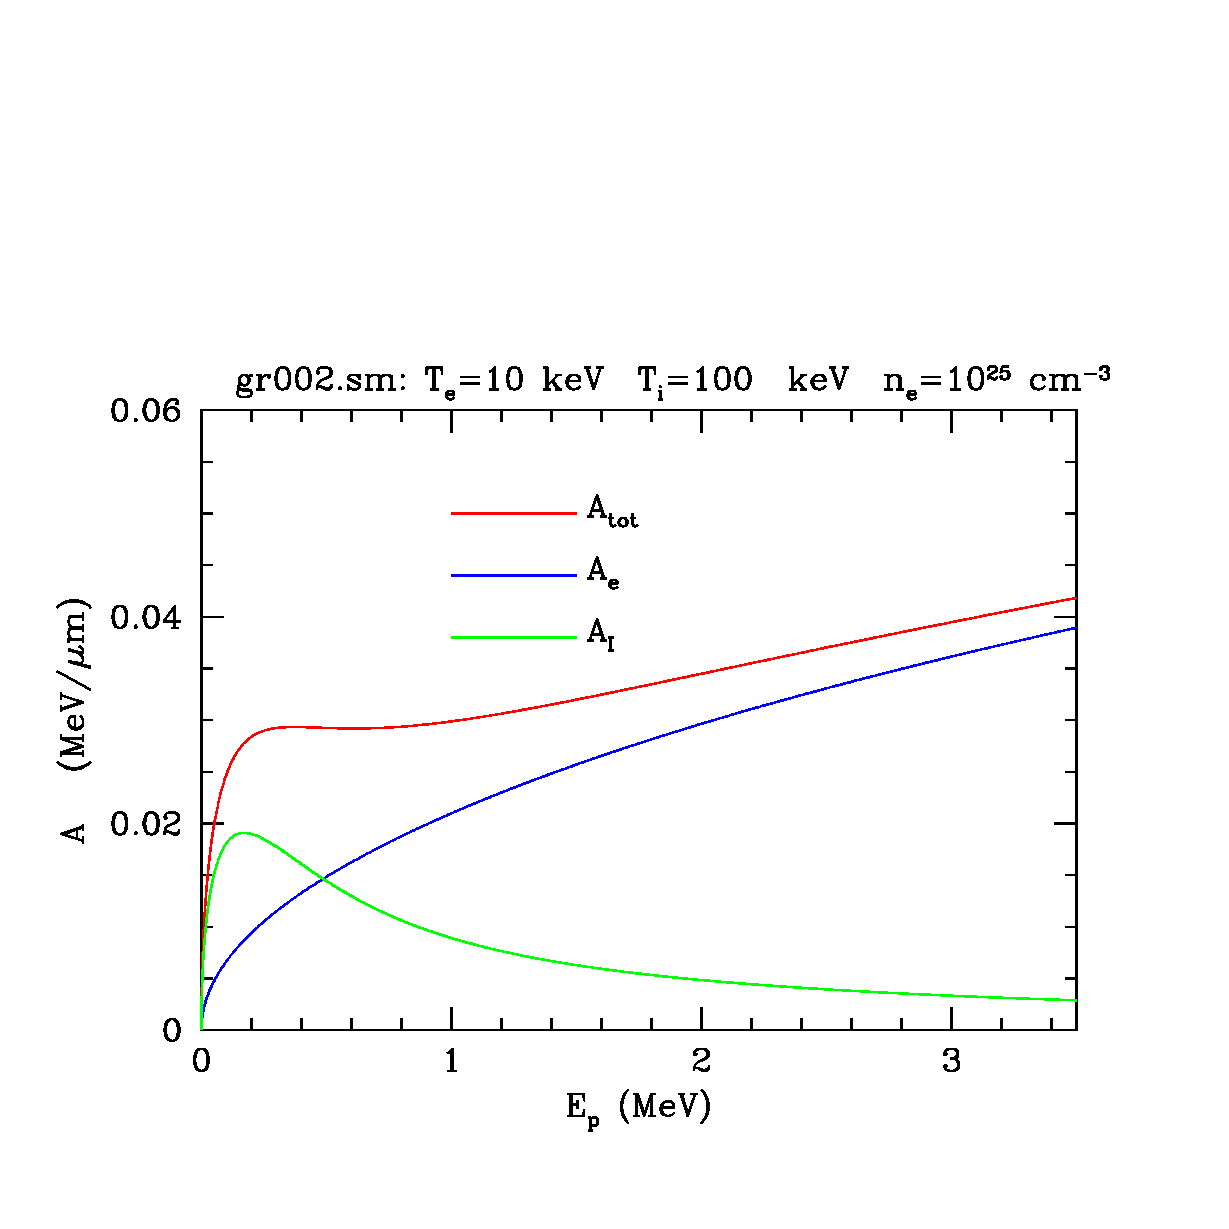
\includegraphics[scale=0.45]{gr002.eps} 
\vskip-0.8cm 
\caption{\footnoteskip  
%%
  Electron and ion components: $n_e=10^{25}\,{\rm cm^{-3}}$,
  $T_e=10\,{\rm keV}$, $T_\smI=100\,{\rm keV}$. [gr002.f90, gr002.sm,
  gr002.dat, gr002.eps]
%%
}
\label{fig:gr002}
\end{figure}
%%

%%
\vskip-2cm 
\begin{figure}[h!]
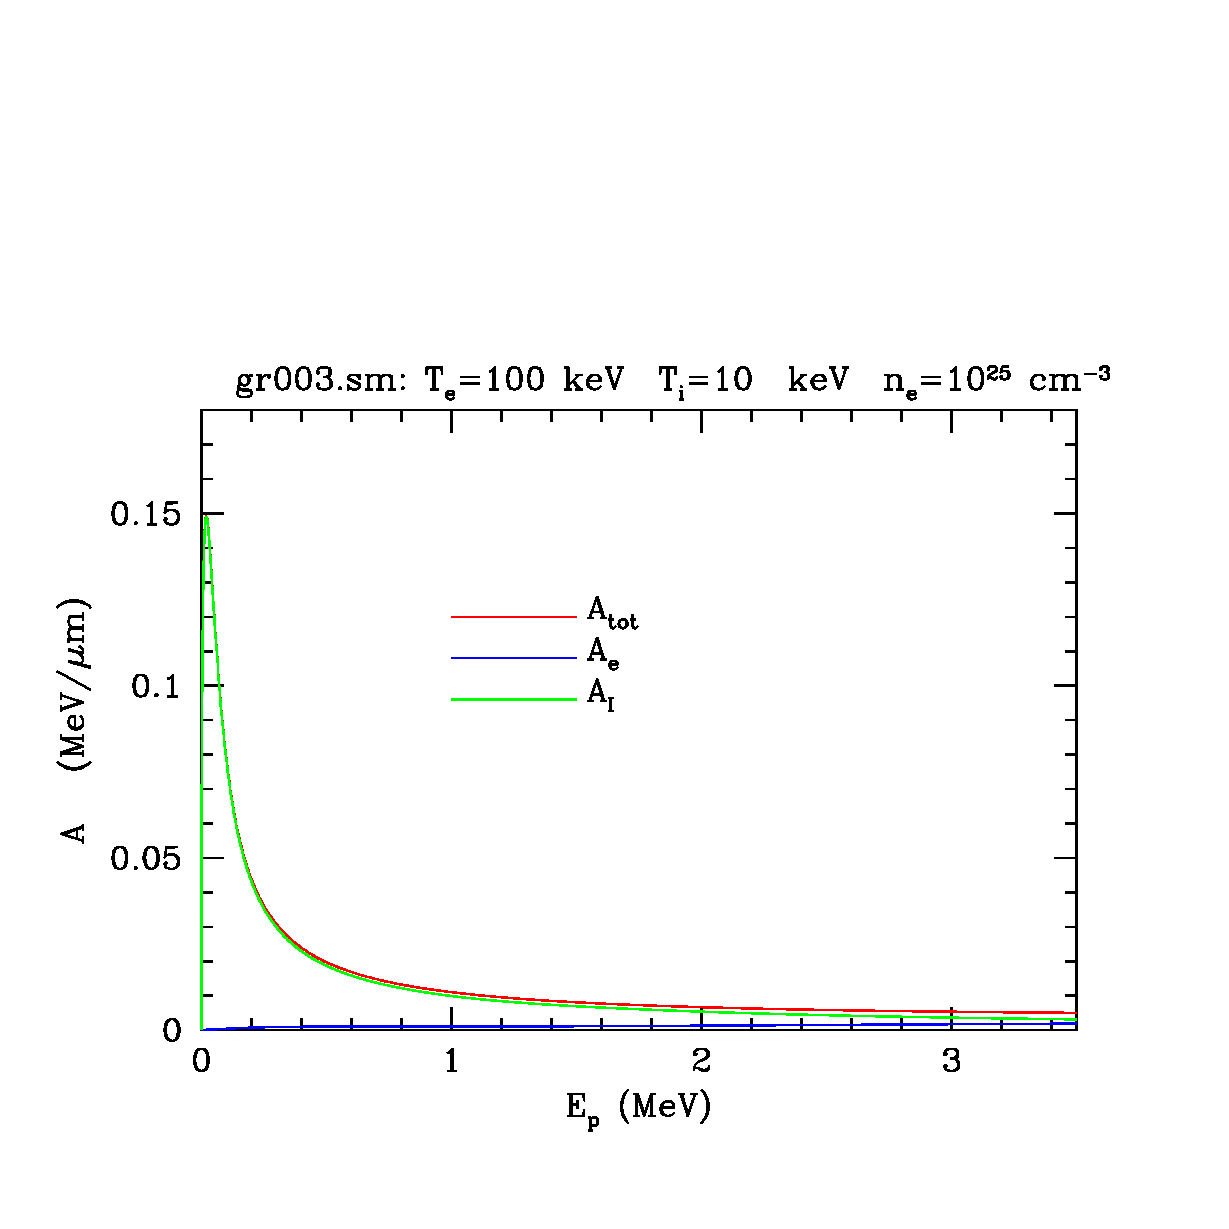
\includegraphics[scale=0.45]{gr003.eps} 
\vskip-0.8cm 
\caption{\footnoteskip  
%%
  Electron and ion components: $n_e=10^{25}\,{\rm cm^{-3}}$,
  $T_e=100\,{\rm keV}$, $T_\smI=10\,{\rm keV}$. [gr003.f90, gr003.sm,
  gr003.dat, gr003.eps]
%%
}
\label{fig:gr003}
\end{figure}
%%

\pagebreak
\clearpage
\section{Small Energy Asymptotic Behavior}

In the small energy limit, the ${\cal A}$-coefficients become:
%%
\begin{eqnarray}
  v_p \to 0 \,: 
  {\cal A}_b(v_p) 
  =  
  \underbrace{~
  \frac{e_p^2\,\kappa_b^2}{4\pi} 
  ~}_{c_1}
  ~
  \underbrace{
  \left( \frac{\beta_b m_b}{2\pi} \right)^{1/2} v_p 
  }_{c_2}
  \cdot
  \left\{ A_b^\smC + A_b^{\Delta Q} \right\} \,,
\label{low}
\end{eqnarray}
%%
with
%%
\begin{eqnarray}
  A_b^\smC 
  &=& 
  \frac{2}{3} \left[ \ln \left( 
  \frac{16\pi}{e_p e_b \, \beta_b \kappa_\smD} \, \frac{m_{pb}}{m_b}
  \right ) - \frac{1}{2} - 2 \gamma \right]
\label{classvzero}
\\[5pt]
  A_b^{\Delta Q} 
  &=& 
  -\bar\eta_{pb}^2 \,\int_0^\infty du \, u \, 
  \exp\left\{ - \frac{3}{2} \bar\eta_{pb}^2 \, u^2 \right\}
  \left[2 \,  {\rm Re} \, \psi\left( 1 + \frac{i}{u} \right) 
  + \ln u^2 \right] \,,
\label{Dq}
\end{eqnarray}
%%
and $\bar \eta_{pb}=e_p e_b/4\pi \hbar \bar v_b$ (note: $\bar v_b^2 = 3 T_b/m_b$). 
The small energy quantum contribution takes separate
forms for electrons and ions:
%%
\begin{eqnarray}
  {\bar\eta_{pe}}^2 \ll 1 \,:&&
  A_e^{\Delta Q} \simeq  - \bar\eta_{pe}^2 \,
  \int_0^\infty du \, u \, 
  \exp\left\{ - \frac{3}{2} \bar\eta_{pe}^2 \, u^2 \right\}
  \left[- 2 \, \gamma  + \ln u^2 \right] 
  =
  \frac{1}{3} \, \ln\left( \frac{3}{2} \,\bar\eta^2_{pe} \right)
  + \gamma \,.
\nonumber\\
\\[10pt]
{\bar\eta_{pi}}^2 \gg 1 \,:&&
  A_i^{\Delta Q}
  \simeq 
  - \frac{\bar\eta_{pi}^2}{6} \,\int_0^\infty du \, u^3 \, 
  \exp\left\{ - \frac{3}{2} \bar\eta_{pi}^2 \, u^2 \right\}
  =  
  - \frac{1}{27} \, {\bar\eta}_{pi}^{\, -2} \,.
\end{eqnarray}
%%
The next figure illustrates the relative size of the classical
contribution ${\cal A}^\smC$ and the total coefficient ${\cal A}={\cal
A}^\smC + {\cal A}^\smQM$. for the density $n_e=10^{25}\,{\rm
cm}^{-3}$. This gives us an idea of the size of the quantum
contribution.
%%
\vskip-2cm 
\begin{figure}[h!]
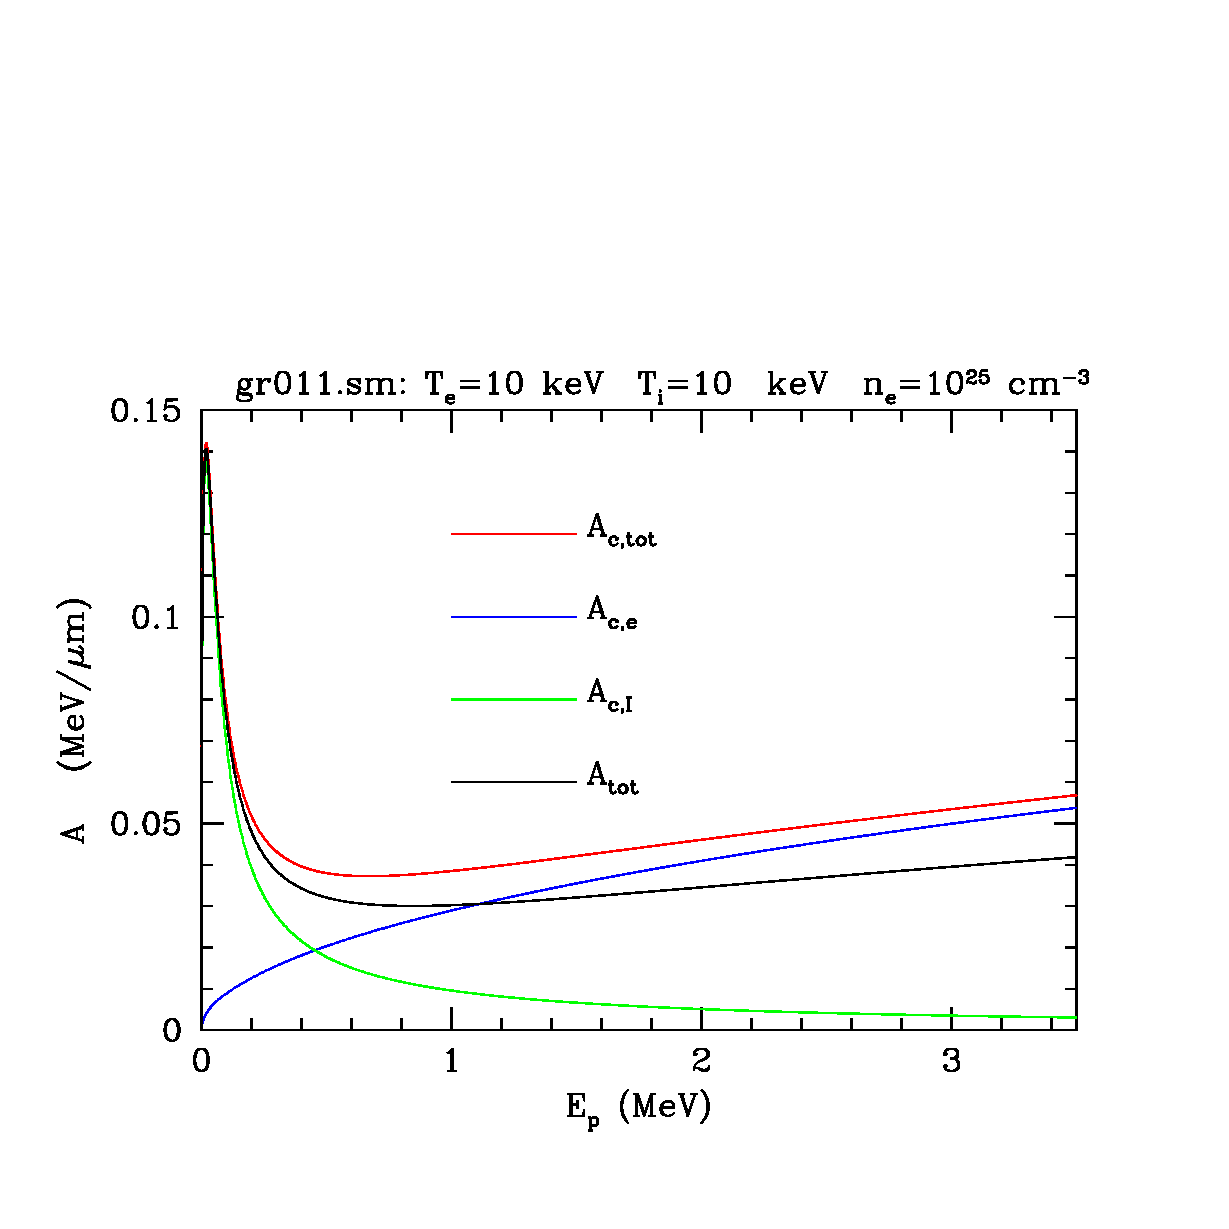
\includegraphics[scale=0.45]{gr011.eps} 
\vskip-0.8cm 
\caption{\footnoteskip  
%%
  The classical contributions to the {\cal A}-coefficient, with the
  total (classical + quantum) in black.  [gr001.f90, gr011.sm,
  gr001.dat, gr011.eps]
%%
}
\label{fig:gr011}
\end{figure}
%%


\pagebreak
\subsection{Ions: Classical and Quantum}

For each of the three cases illustrated in
Figs.~\ref{fig:gr001}--\ref{fig:gr003}, we will now look at the ion
contributions for the classical and quantum cases.

\subsubsection{Temperatures $T_e=10\,{\rm keV}$ and $T_\smI=10\,{\rm keV}$}

%%
\vskip-2cm 
\begin{figure}[h!]
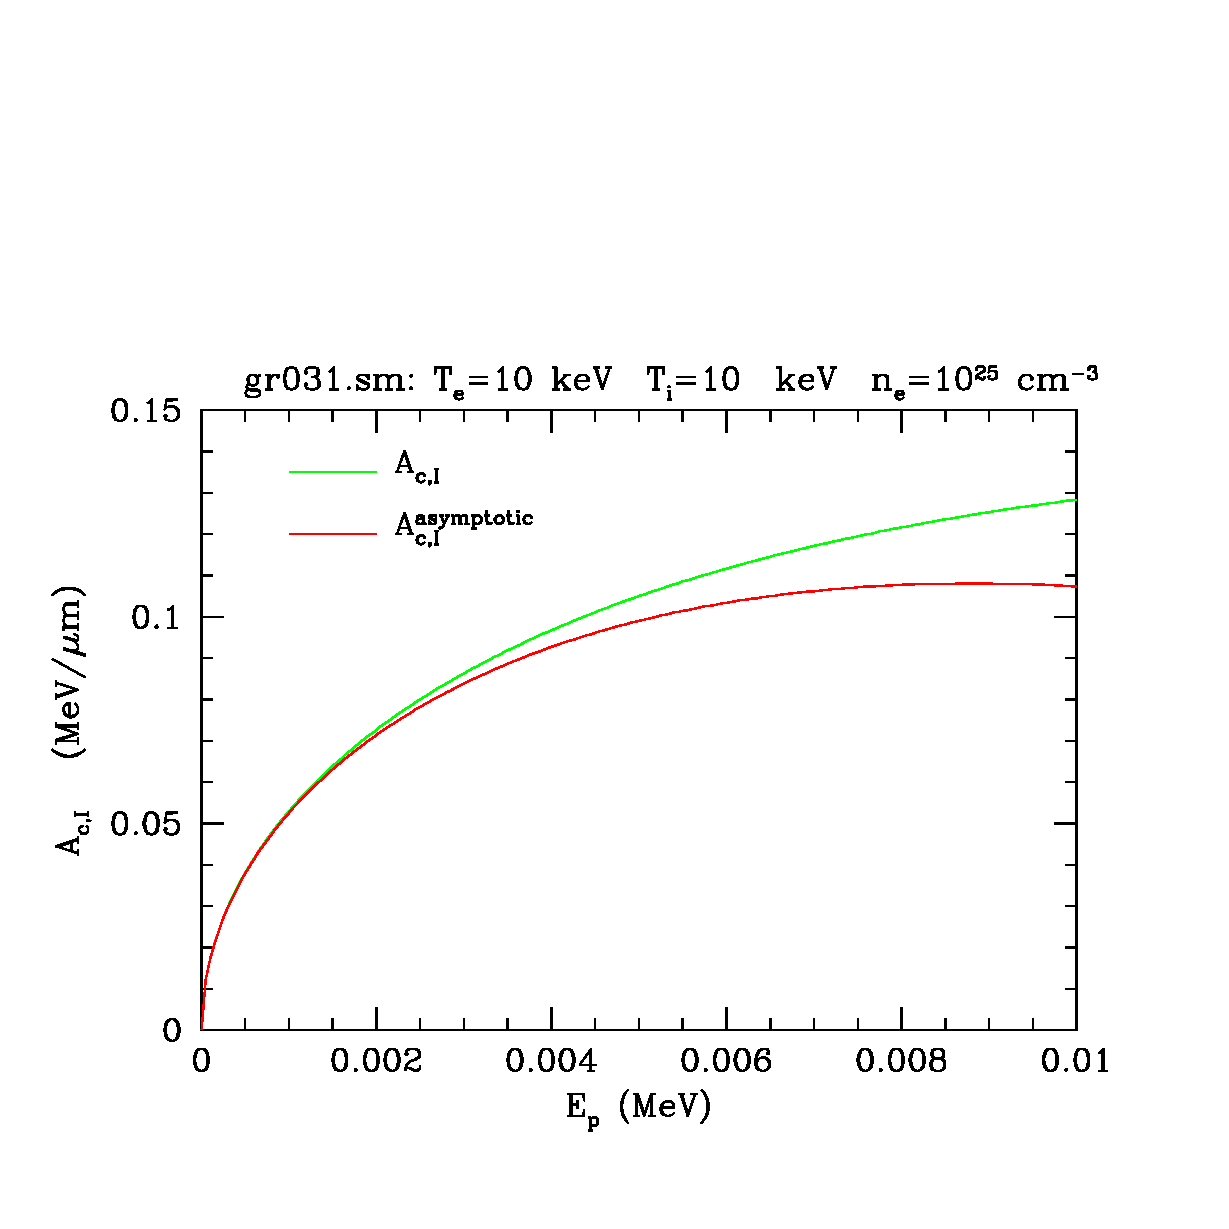
\includegraphics[scale=0.45]{gr031.eps} 
\vskip-0.8cm 
\caption{\footnoteskip  
%%
  Asymptotic classical ion contribution at low energies. [gr001.f90,
  gr031.sm, gr001.dat, gr001.smallE.dat, gr031.eps]
%%
}
\label{fig:gr031}
\end{figure}
%%

%%
\vskip-2.0cm 
\begin{figure}[h!]
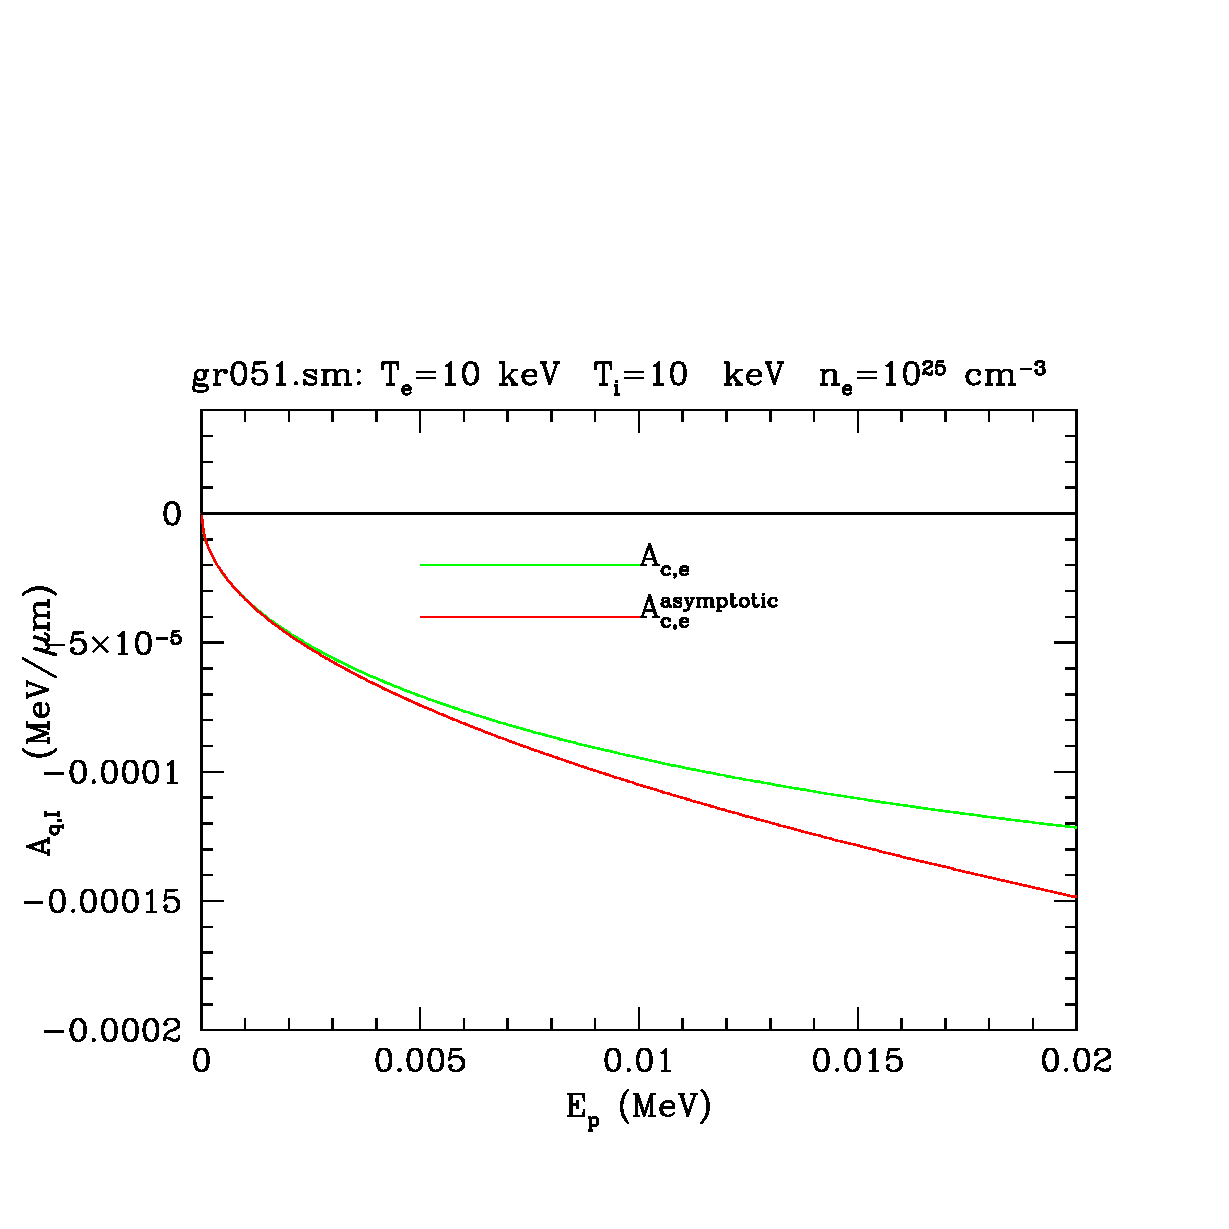
\includegraphics[scale=0.45]{gr051.eps} 
\vskip-0.8cm 
\caption{\footnoteskip  
%%
  Asymptotic quantum ion contribution at low energies. [gr001.f90,
  gr051.sm, gr001.dat, gr001.smallE.dat, gr051.eps]
%%
}
\label{fig:gr051}
\end{figure}
%%



\pagebreak
\subsubsection{Temperatures $T_e=10\,{\rm keV}$ and $T_\smI=100\,{\rm keV}$}

%%
\vskip-2cm 
\begin{figure}[h!]
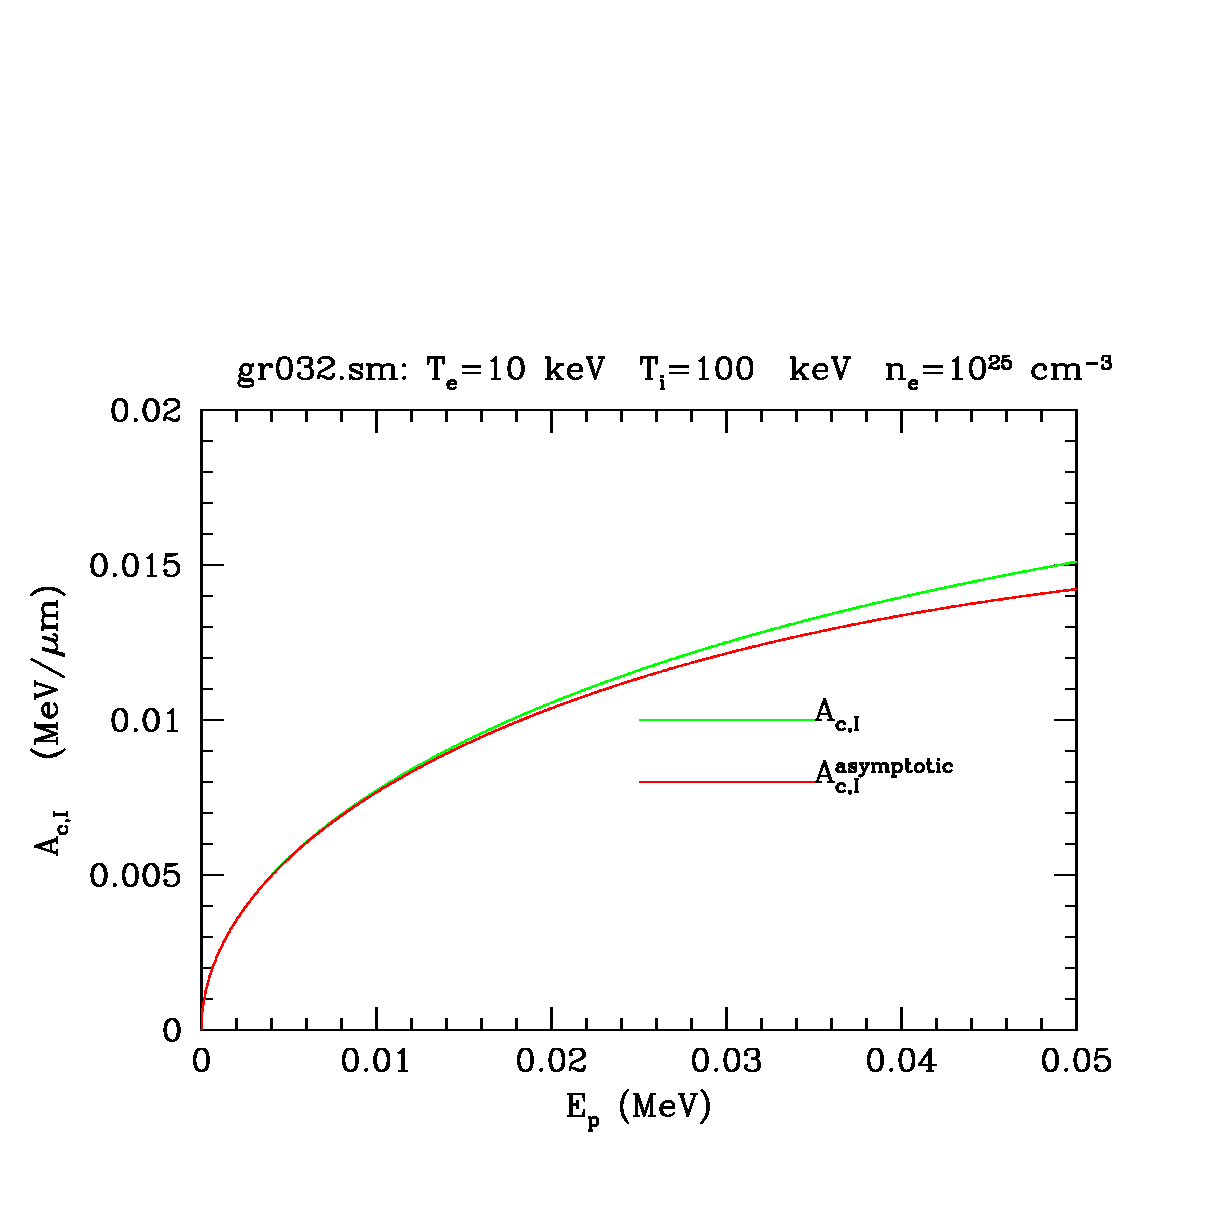
\includegraphics[scale=0.45]{gr032.eps} 
\vskip-0.8cm 
\caption{\footnoteskip  
%%
  Asymptotic classical ion contribution at low energies. [gr002.f90,
  gr032.sm, gr002.dat, gr002.smallE.dat, gr032.eps]
%%
}
\label{fig:gr032}
\end{figure}
%%

%%
\vskip-2cm 
\begin{figure}[h!]
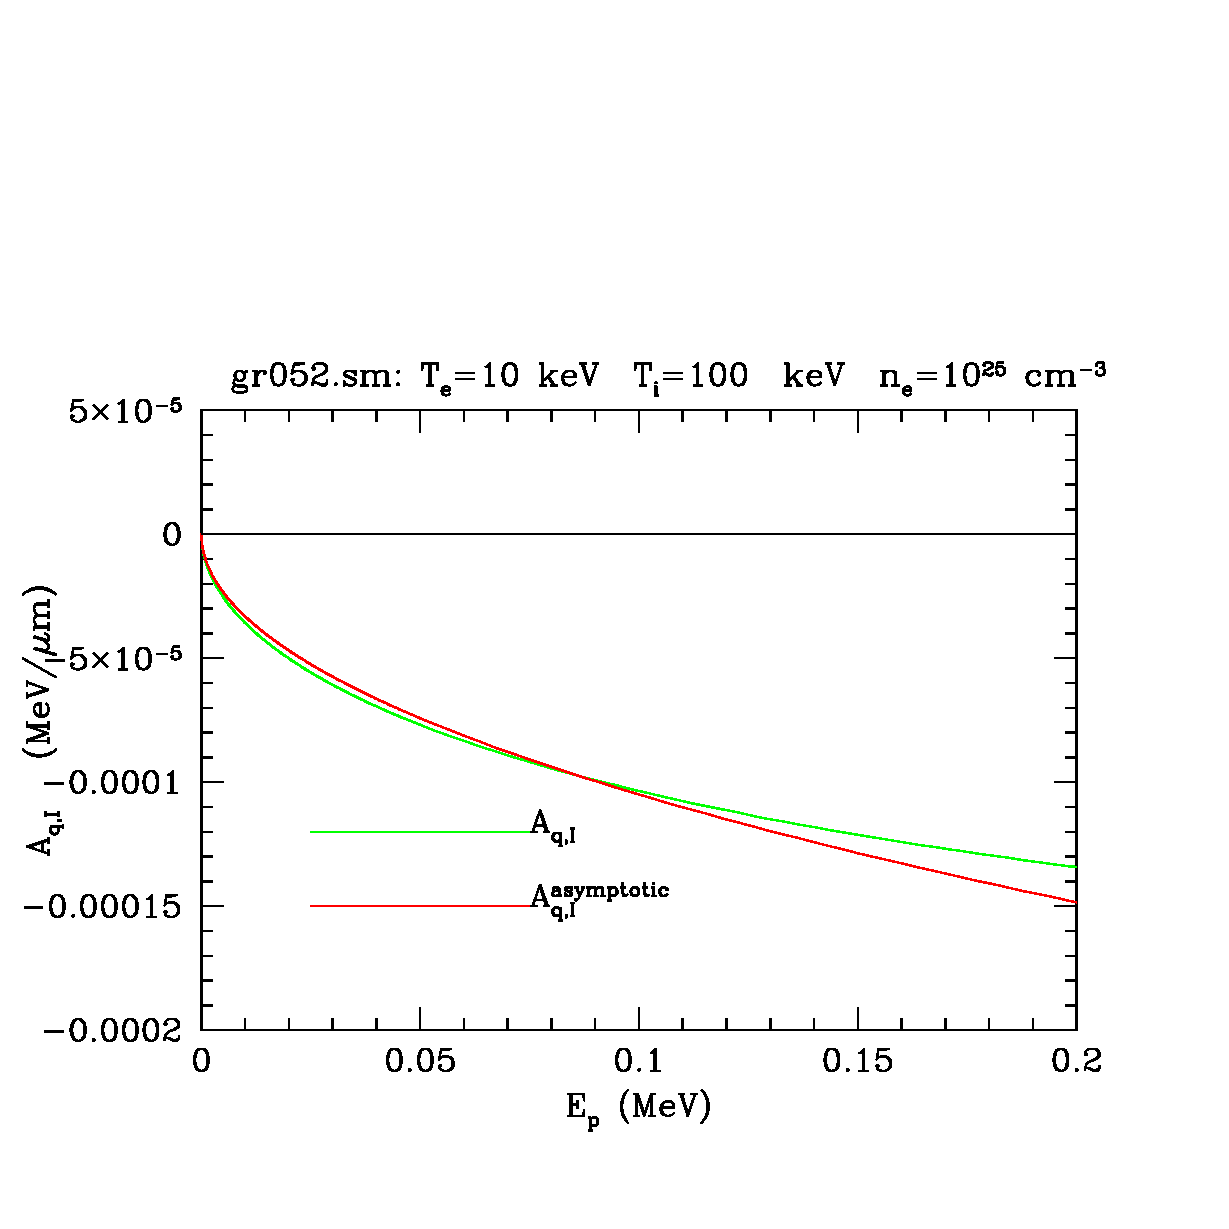
\includegraphics[scale=0.45]{gr052.eps} 
\vskip-0.8cm 
\caption{\footnoteskip  
%%
  Asymptotic quantum ion contribution at low energies. [gr002.f90,
  gr052.sm, gr002.dat, gr002.smallE.dat, gr052.eps]
%%
}
\label{fig:gr052}
\end{figure}
%%


\pagebreak
\subsubsection{Temperatures $T_e=100\,{\rm keV}$ and $T_\smI=10\,{\rm keV}$}

%%
\vskip-2cm 
\begin{figure}[h!]
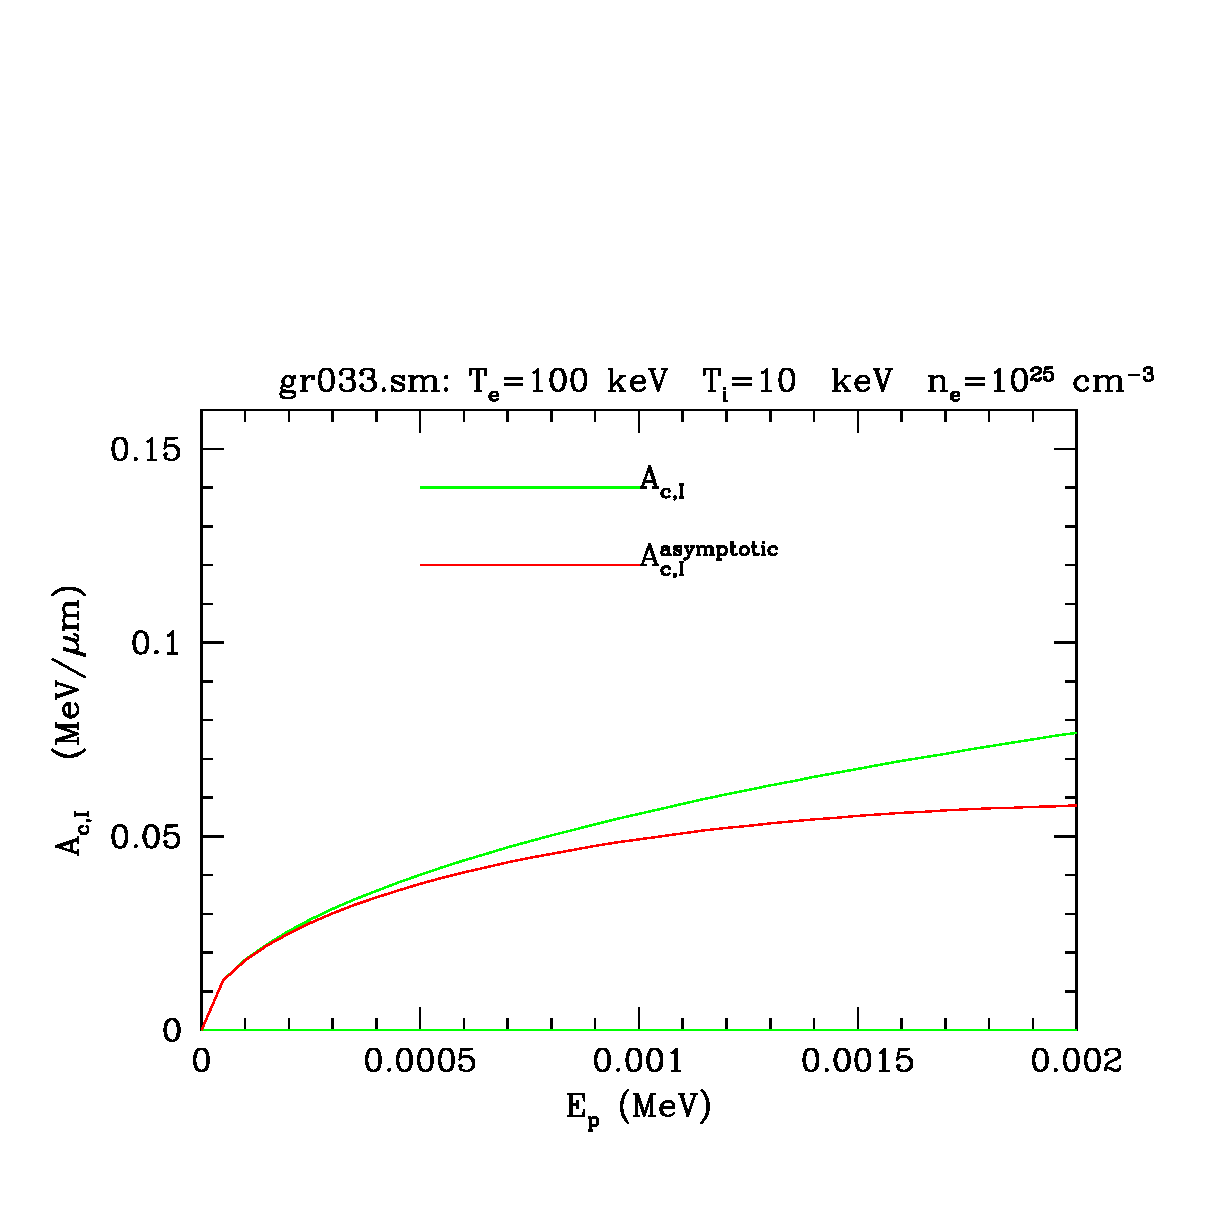
\includegraphics[scale=0.45]{gr033.eps} 
\vskip-0.8cm 
\caption{\footnoteskip  
%%
  Asymptotic classical ion contribution at low energies. [gr003.f90,
  gr033.sm, gr003.dat, gr003.smallE.dat, gr033.eps]
%%
}
\label{fig:gr033}
\end{figure}
%%

%%
\vskip-2cm 
\begin{figure}[h!]
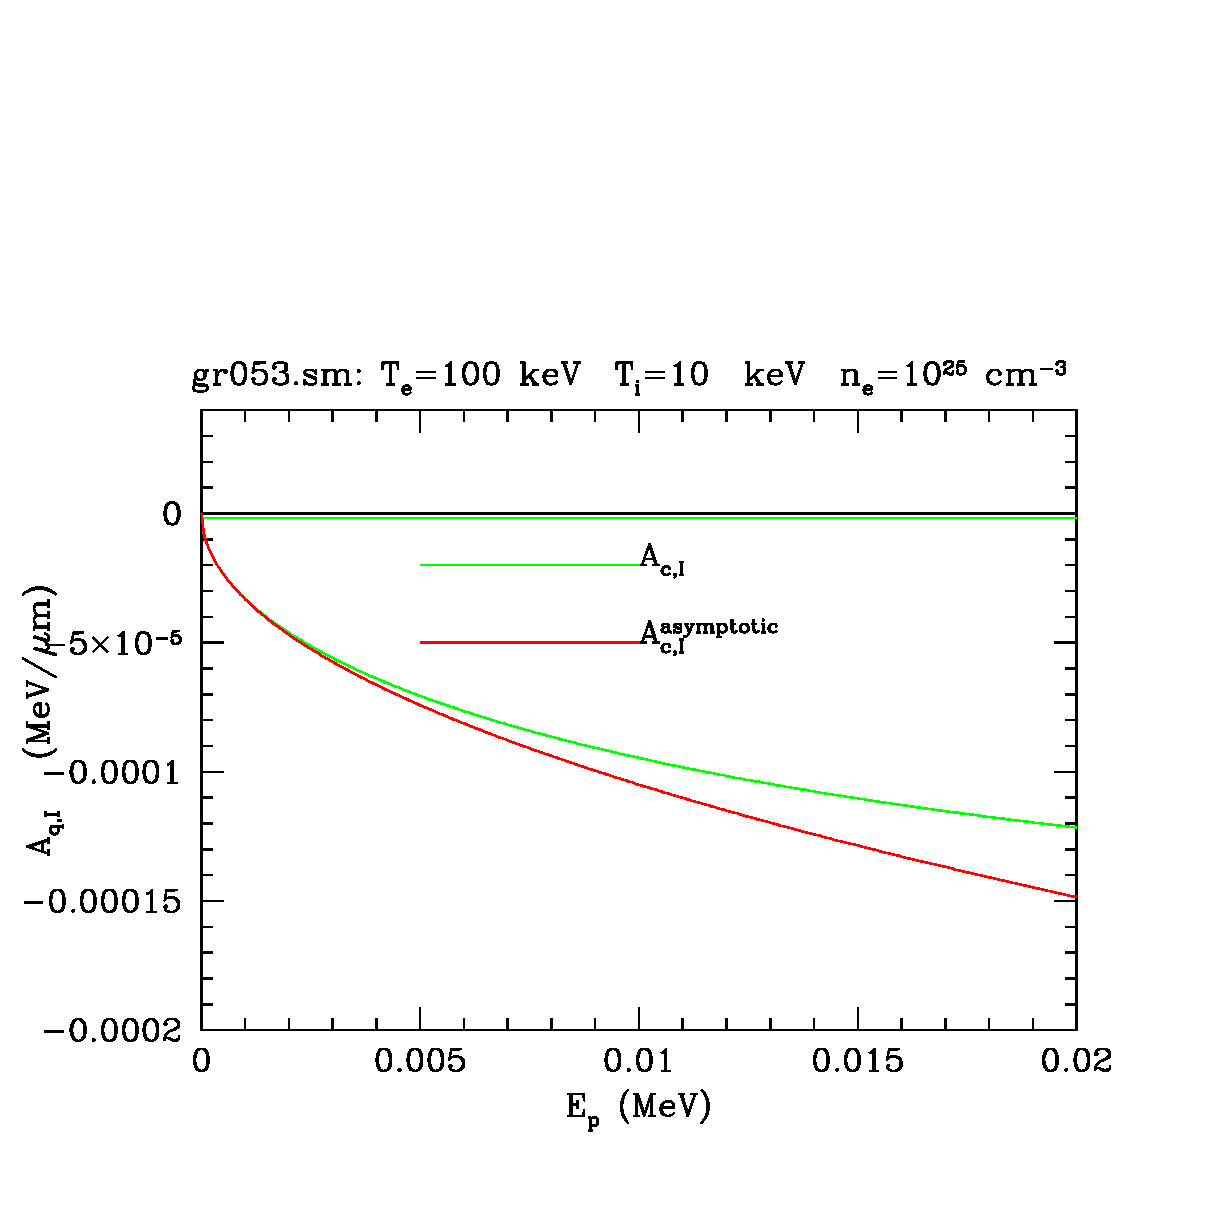
\includegraphics[scale=0.45]{gr053.eps} 
\vskip-0.8cm 
\caption{\footnoteskip  
%%
  Asymptotic quantum ion contribution at low energies. [gr003.f90,
  gr053.sm, gr003.dat, gr003.smallE.dat, gr053.eps]
%%
}
\label{fig:gr053}
\end{figure}
%%


\pagebreak
\subsection{Electrons: Classical and Quantum}

For each of the three cases illustrated in
Figs.~\ref{fig:gr001}--\ref{fig:gr003}, we will now look at the
electron contributions for the classical and quantum cases.

\subsubsection{Temperatures $T_e=10\,{\rm keV}$ and $T_\smI=10\,{\rm keV}$}

%%
\vskip-2cm 
\begin{figure}[h!]
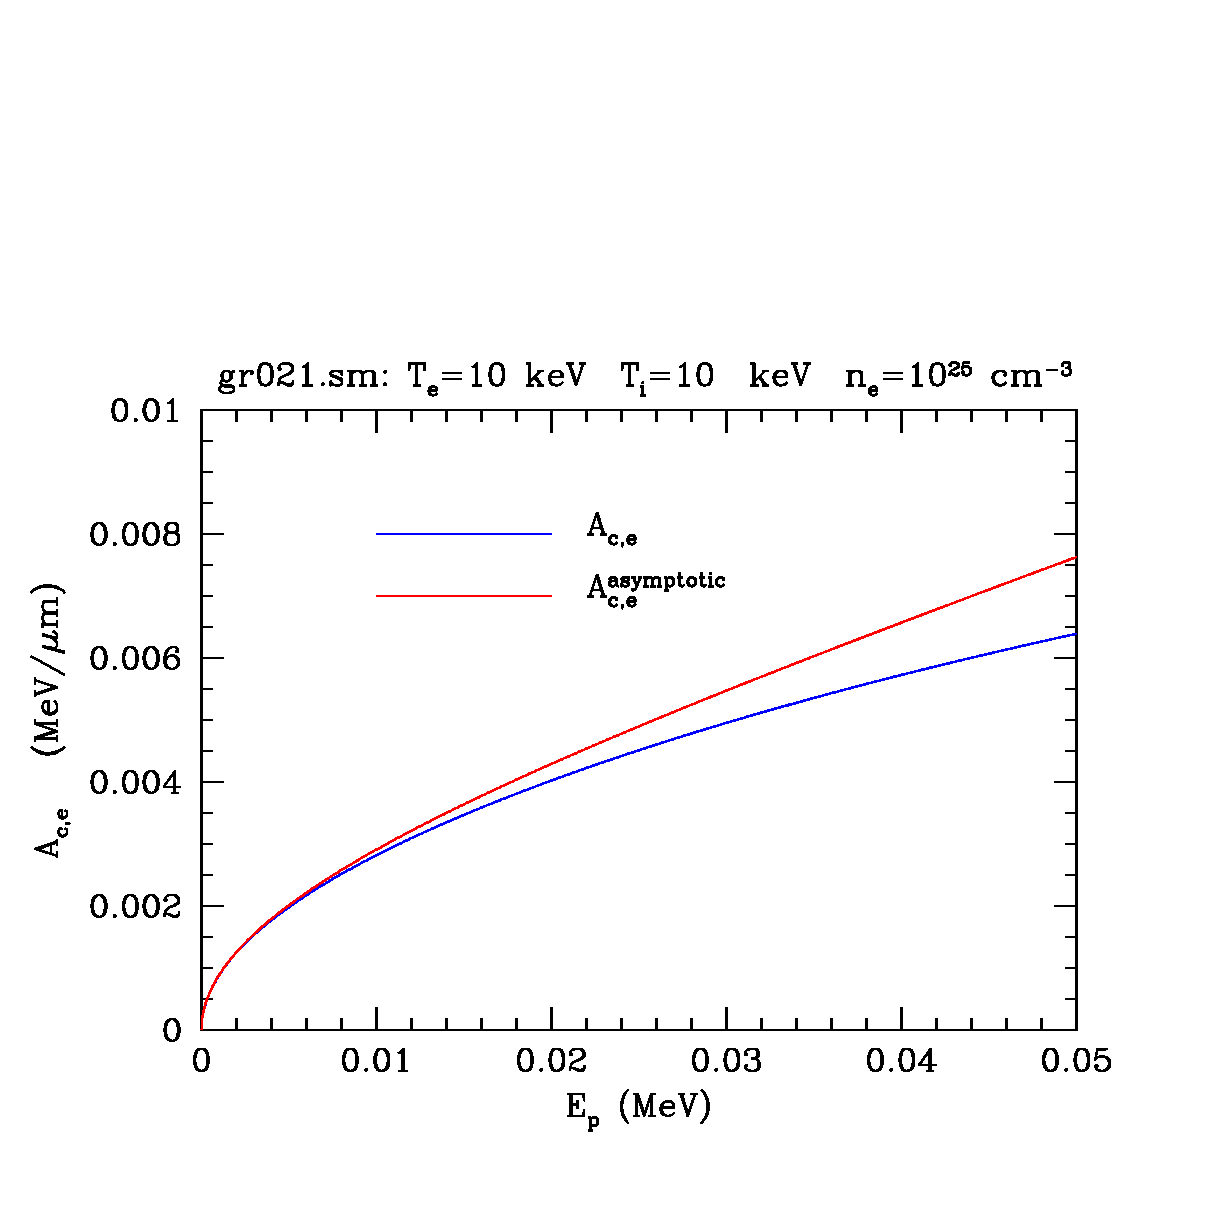
\includegraphics[scale=0.45]{gr021.eps} 
\vskip-0.8cm 
\caption{\footnoteskip  
%%
  Asymptotic classical electron contribution at low
  energies. [gr001.f90, gr021.sm, gr001.dat, gr001.smallE.dat,
  gr021.eps]
%%
}
\label{fig:gr021}
\end{figure}
%%

%%
\vskip-2cm 
\begin{figure}[h!]
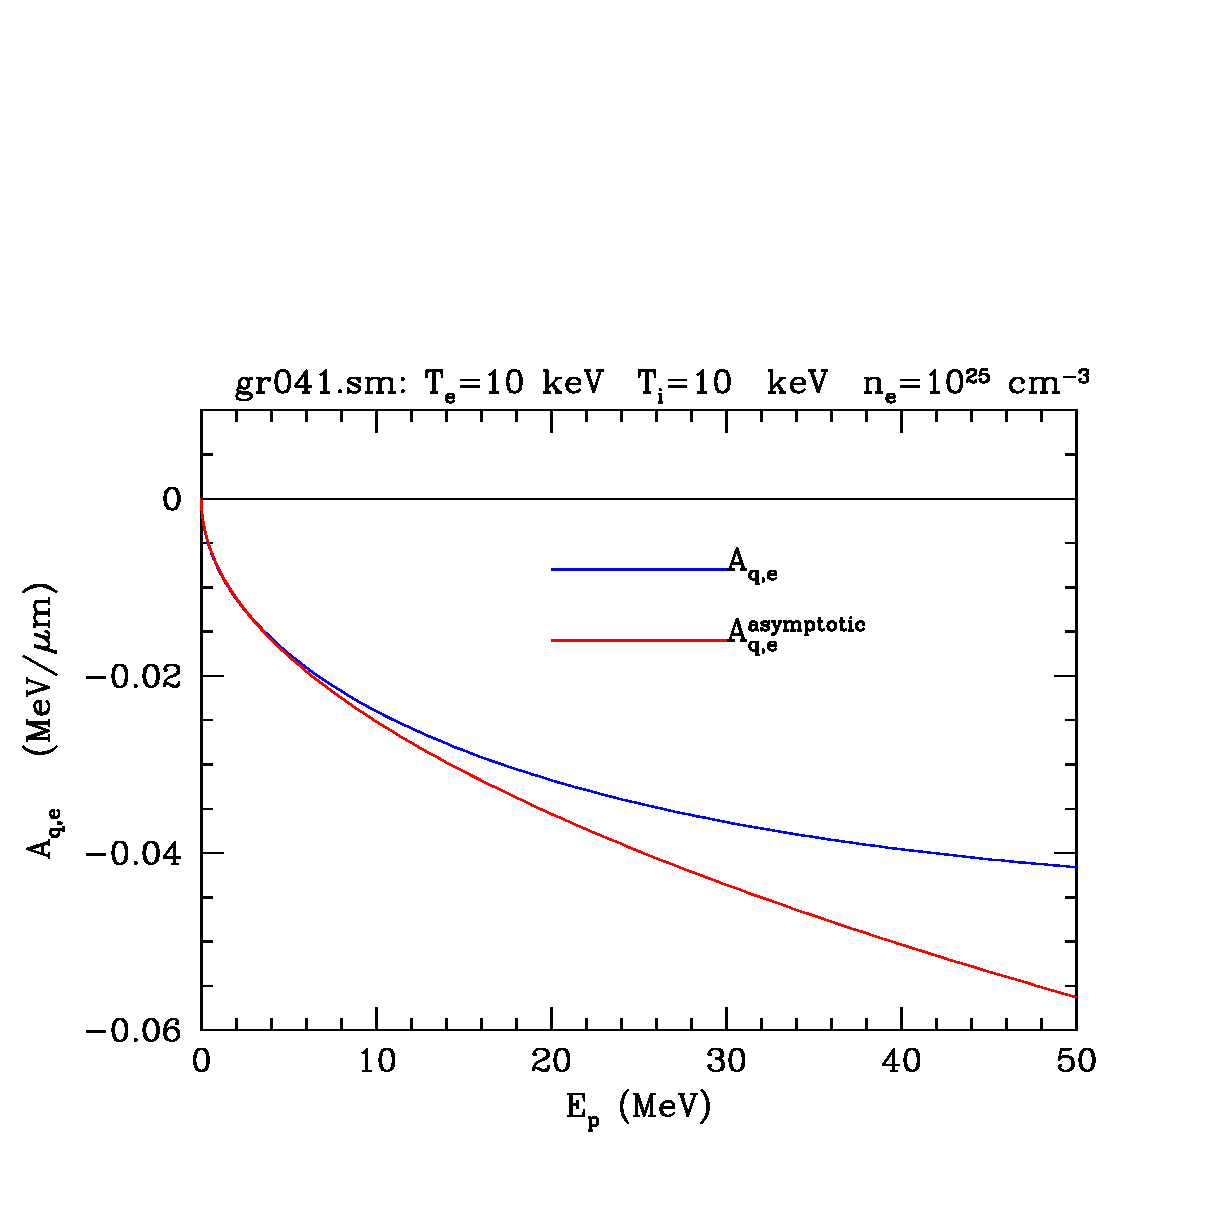
\includegraphics[scale=0.45]{gr041.eps} 
\vskip-0.8cm 
\caption{\footnoteskip  
%%
  Asymptotic quantum electron contribution at low
  energies. [gr001.f90, gr041.sm, gr001.dat, gr001.smallE.dat,
  gr041.eps]
%%
}
\label{fig:gr041}
\end{figure}
%%


\pagebreak
\subsubsection{Temperatures $T_e=10\,{\rm keV}$ and $T_\smI=100\,{\rm keV}$}

%%
\vskip-2cm 
\begin{figure}[h!]
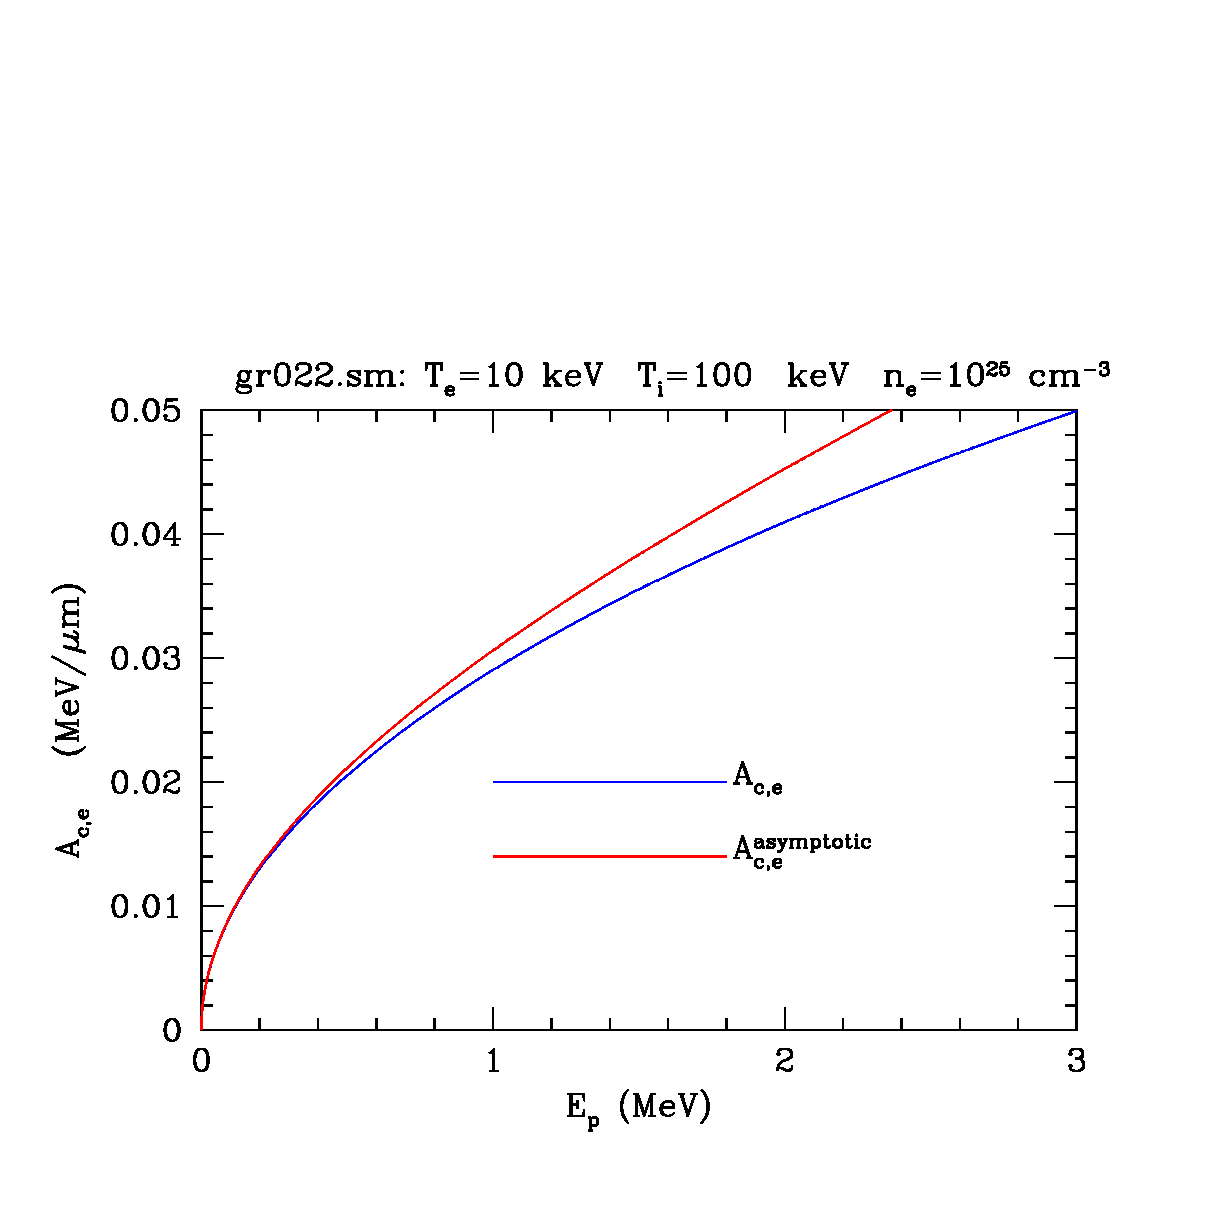
\includegraphics[scale=0.45]{gr022.eps} 
\vskip-0.5cm 
\caption{\footnoteskip  
%%
  Asymptotic classical electron contribution at low
  energies. [gr002.f90, gr022.sm, gr002.dat, gr002.smallE.dat,
  gr022.eps]
%%
}
\label{fig:gr022}
\end{figure}
%%

%%
\vskip-2cm 
\begin{figure}[h!]
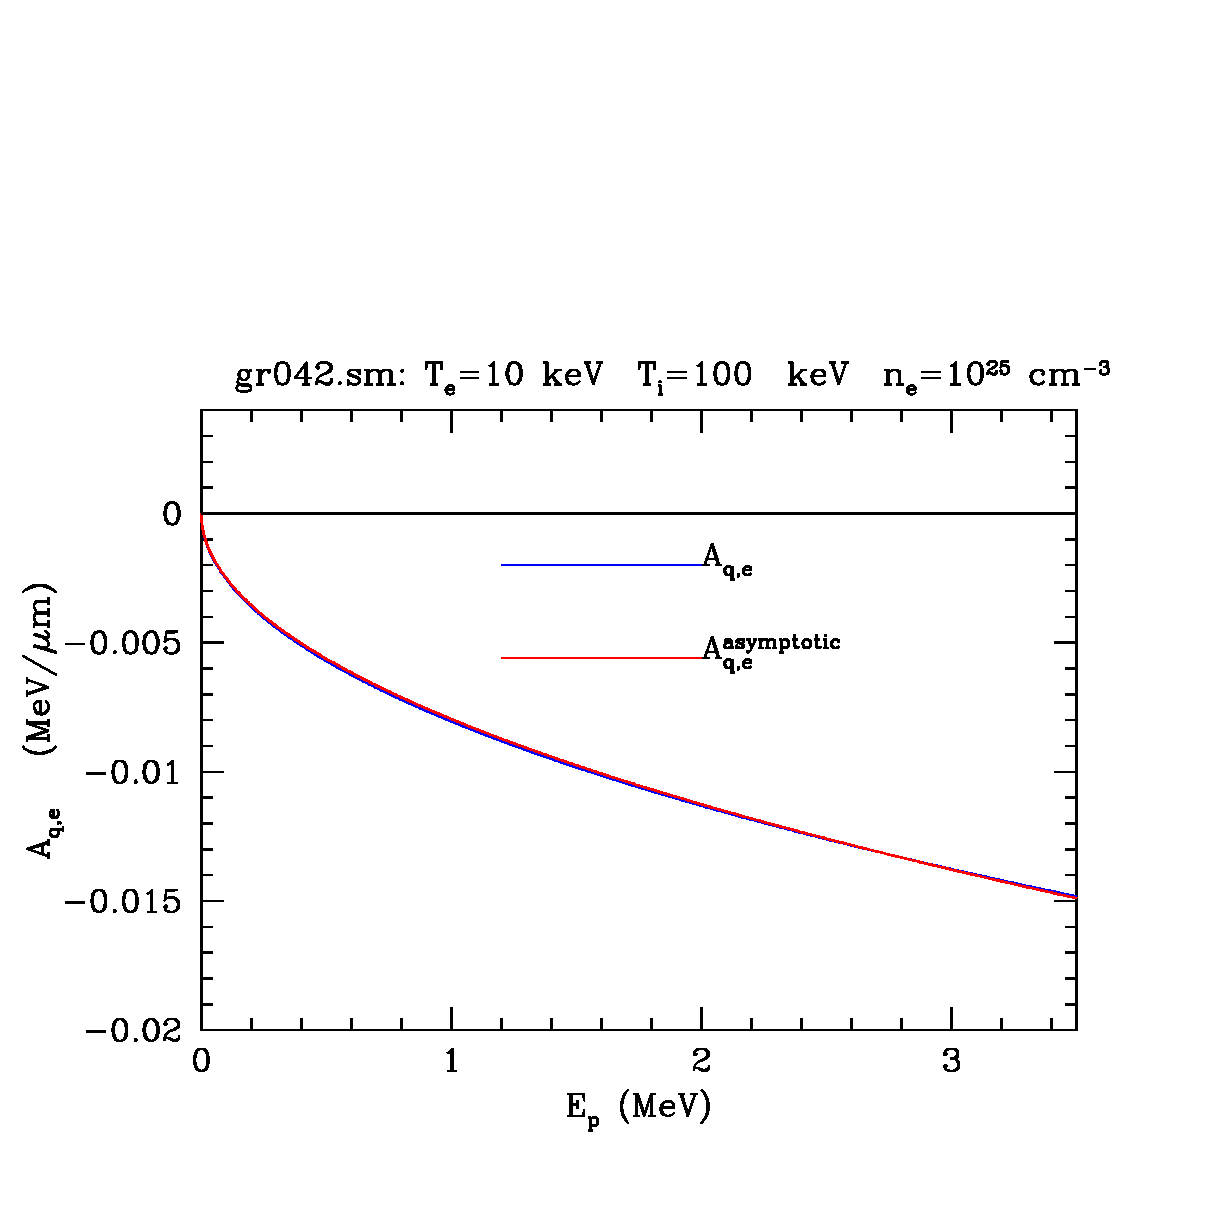
\includegraphics[scale=0.45]{gr042.eps} 
\vskip-0.8cm 
\caption{\footnoteskip  
%%
  Asymptotic quantum electron contribution at low
  energies. [gr002.f90, gr042.sm, gr002.dat, gr002.smallE.dat,
  gr042.eps]
%%
}
\label{fig:gr042}
\end{figure}
%%


\pagebreak
\subsubsection{Temperatures $T_e=100\,{\rm keV}$ and $T_\smI=10\,{\rm keV}$}

%%
\vskip-2cm 
\begin{figure}[h!]
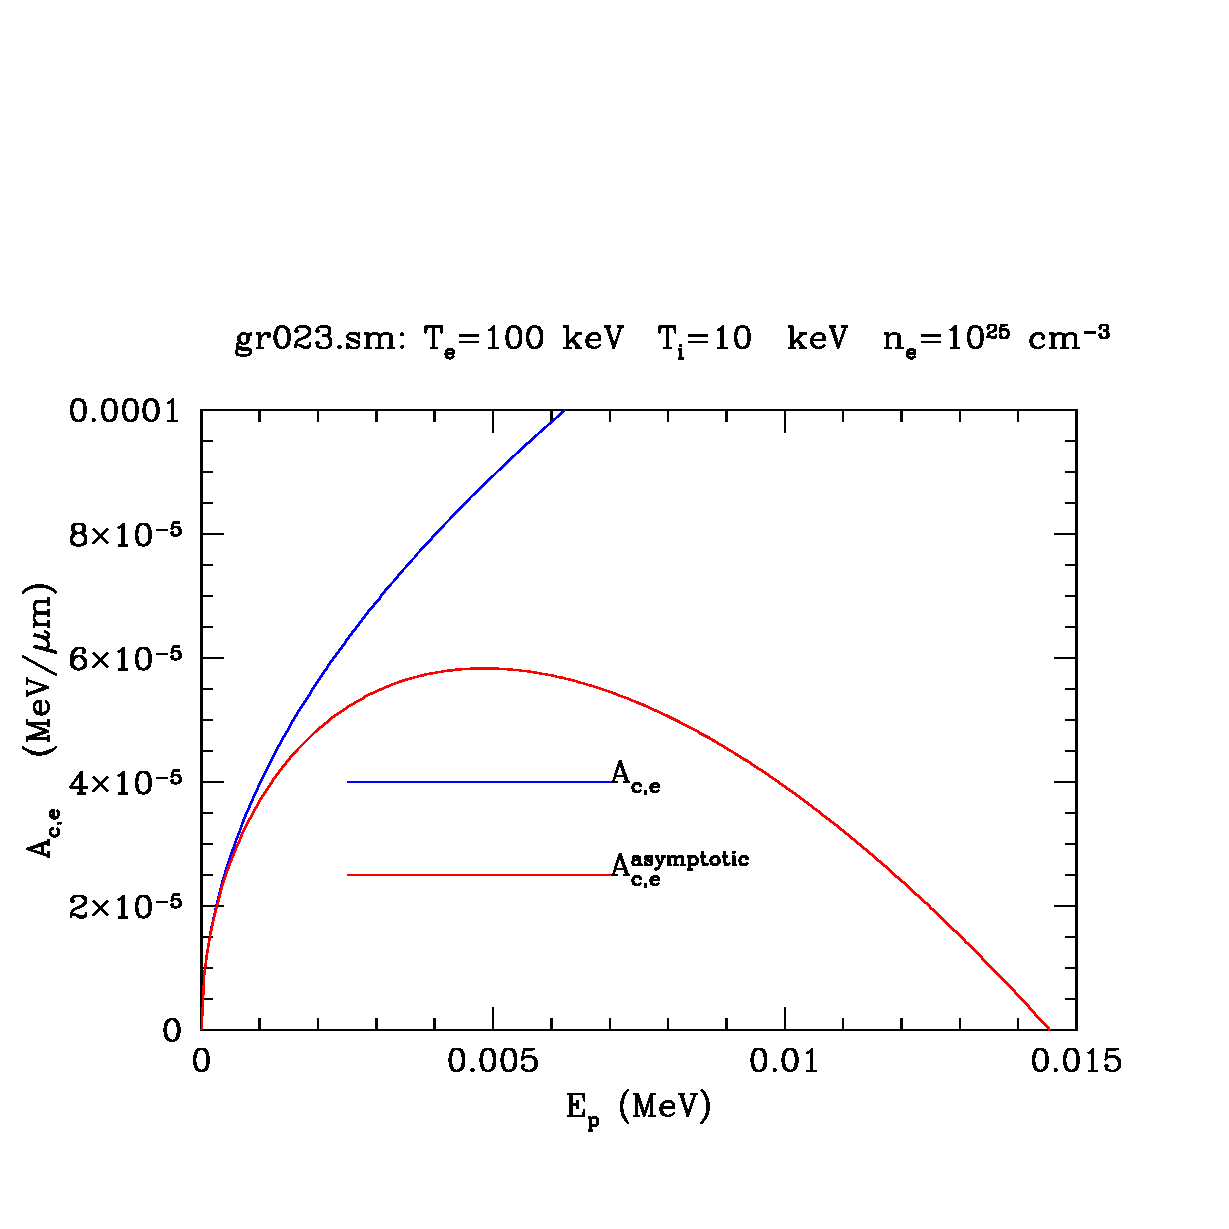
\includegraphics[scale=0.45]{gr023.eps} 
\vskip-0.5cm 
\caption{\footnoteskip  
%%
  Asymptotic classical electron contribution at low
  energies. [gr003.f90, gr023.sm, gr003.dat, gr003.smallE.dat,
  gr023.eps]
%%
}
\label{fig:gr023}
\end{figure}
%%

%%
\vskip-2cm 
\begin{figure}[h!]
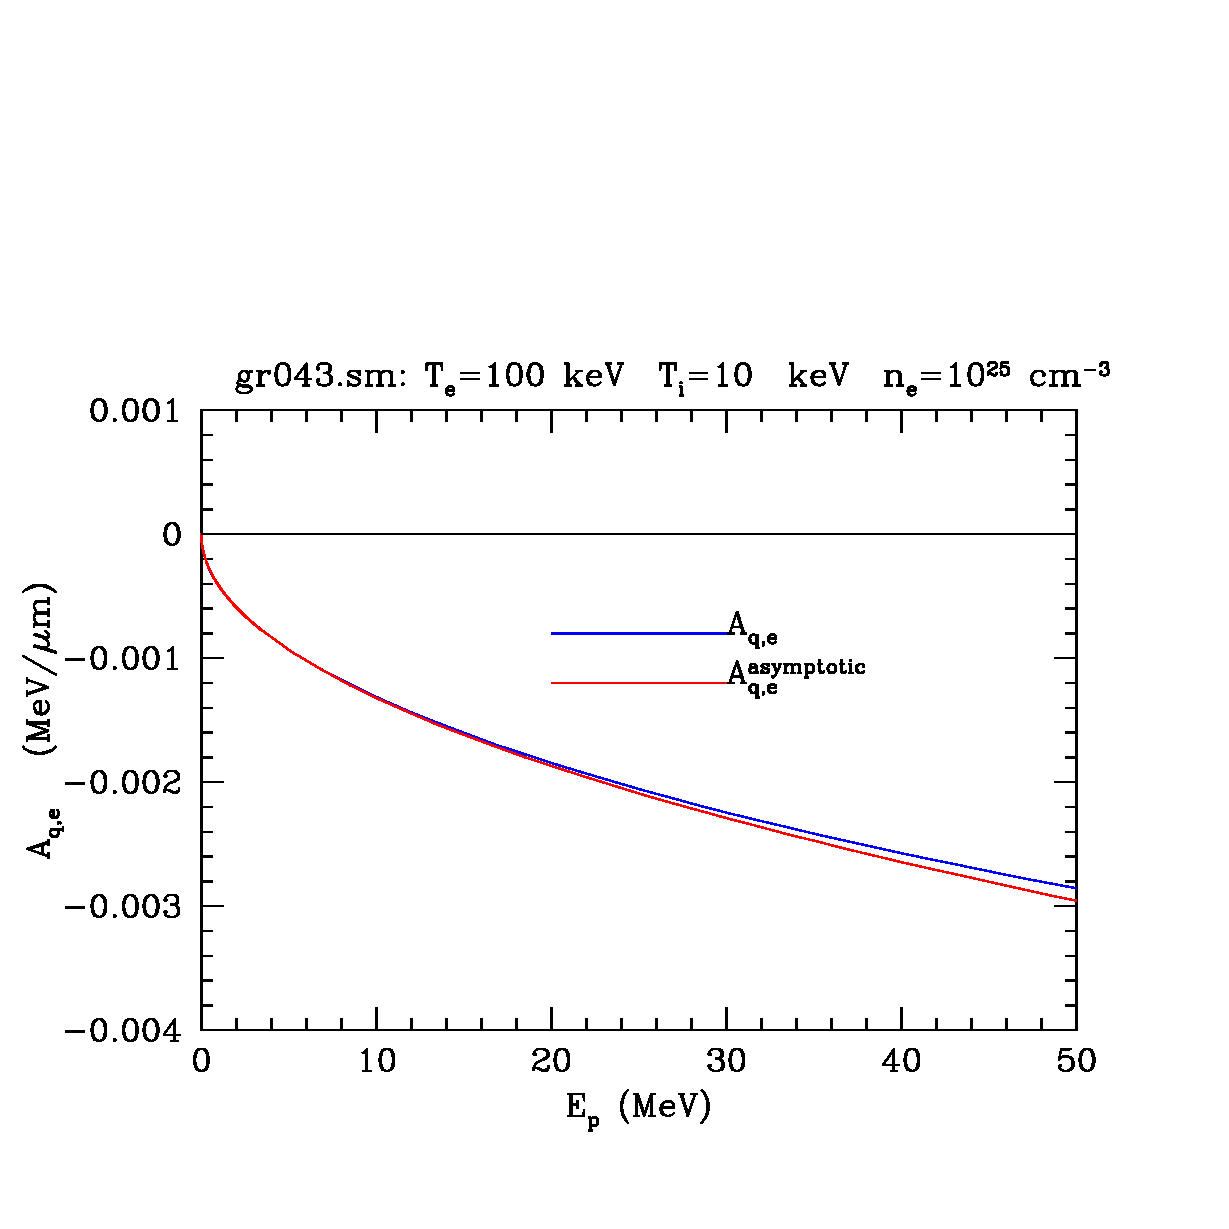
\includegraphics[scale=0.45]{gr043.eps} 
\vskip-0.8cm 
\caption{\footnoteskip  
%%
  Asymptotic quantum electron contribution at low
  energies. [gr003.f90, gr043.sm, gr003.dat, gr003.smallE.dat,
  gr043.eps]
%%
}
\label{fig:gr043}
\end{figure}
%%



\pagebreak
\subsection{Total Electron and Ion Contributions}


\subsubsection{Temperatures $T_e=10\,{\rm keV}$ and $T_\smI=10\,{\rm keV}$}

%%
\vskip-2cm 
\begin{figure}[h!]
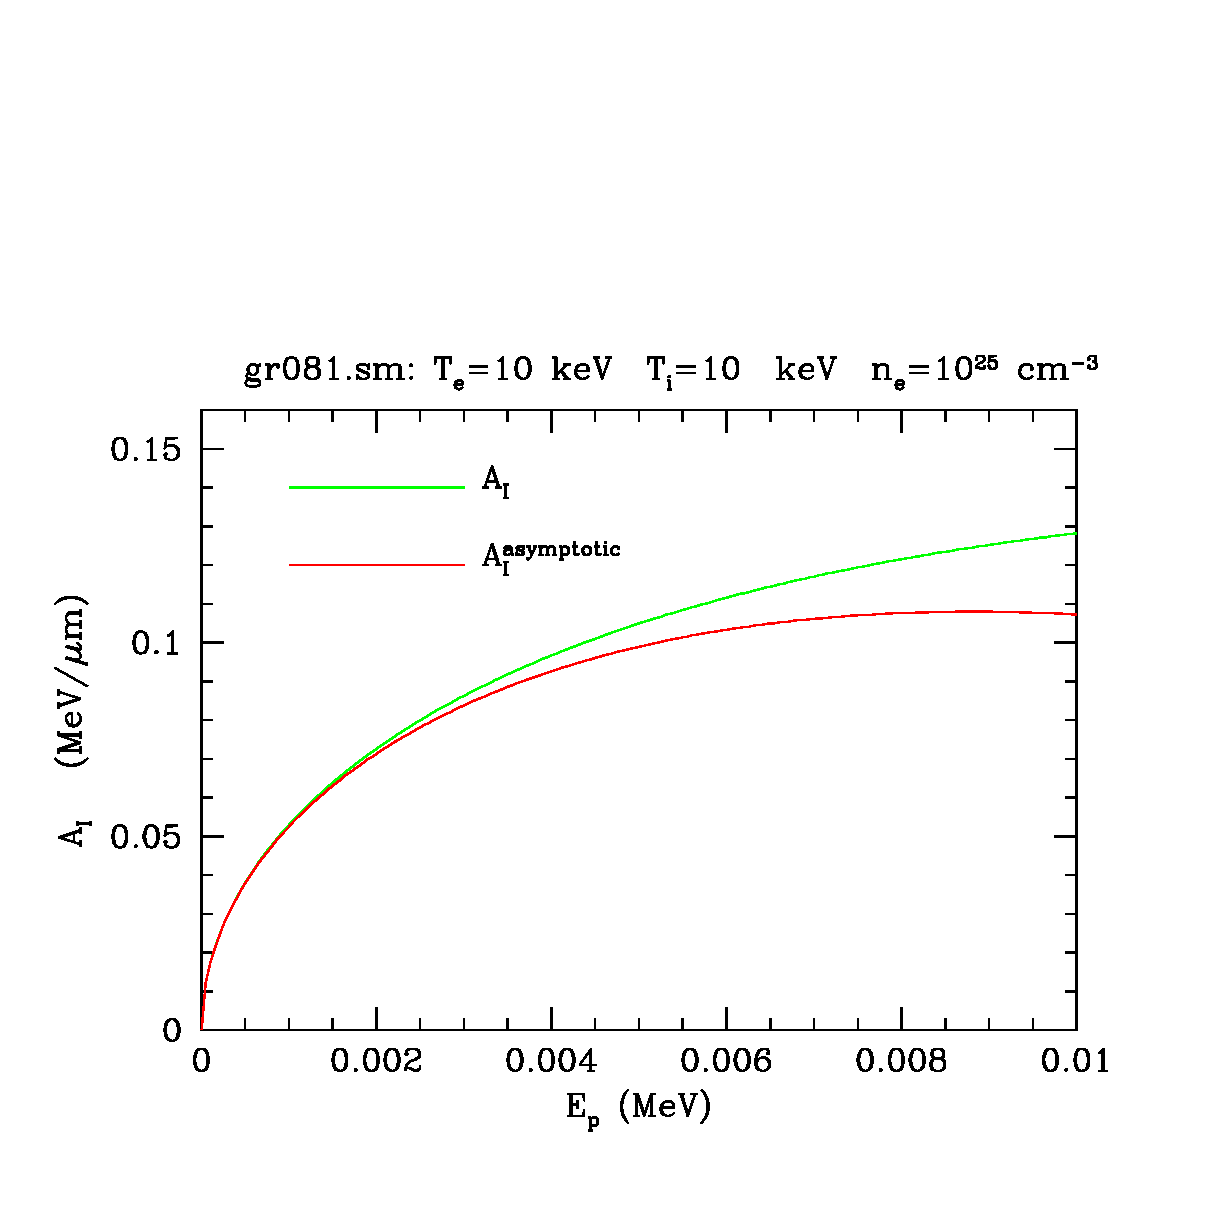
\includegraphics[scale=0.45]{gr081.eps} 
\vskip-0.8cm 
\caption{\footnoteskip  
%%
  Total asymptotic ion contribution at low energies. 
 [gr001.f90, gr081.sm,
    gr001.dat, gr001.smallE.dat, gr081.eps]
%%
}
\label{fig:gr081}
\end{figure}
%%

%%
\vskip-2cm 
\begin{figure}[h!]
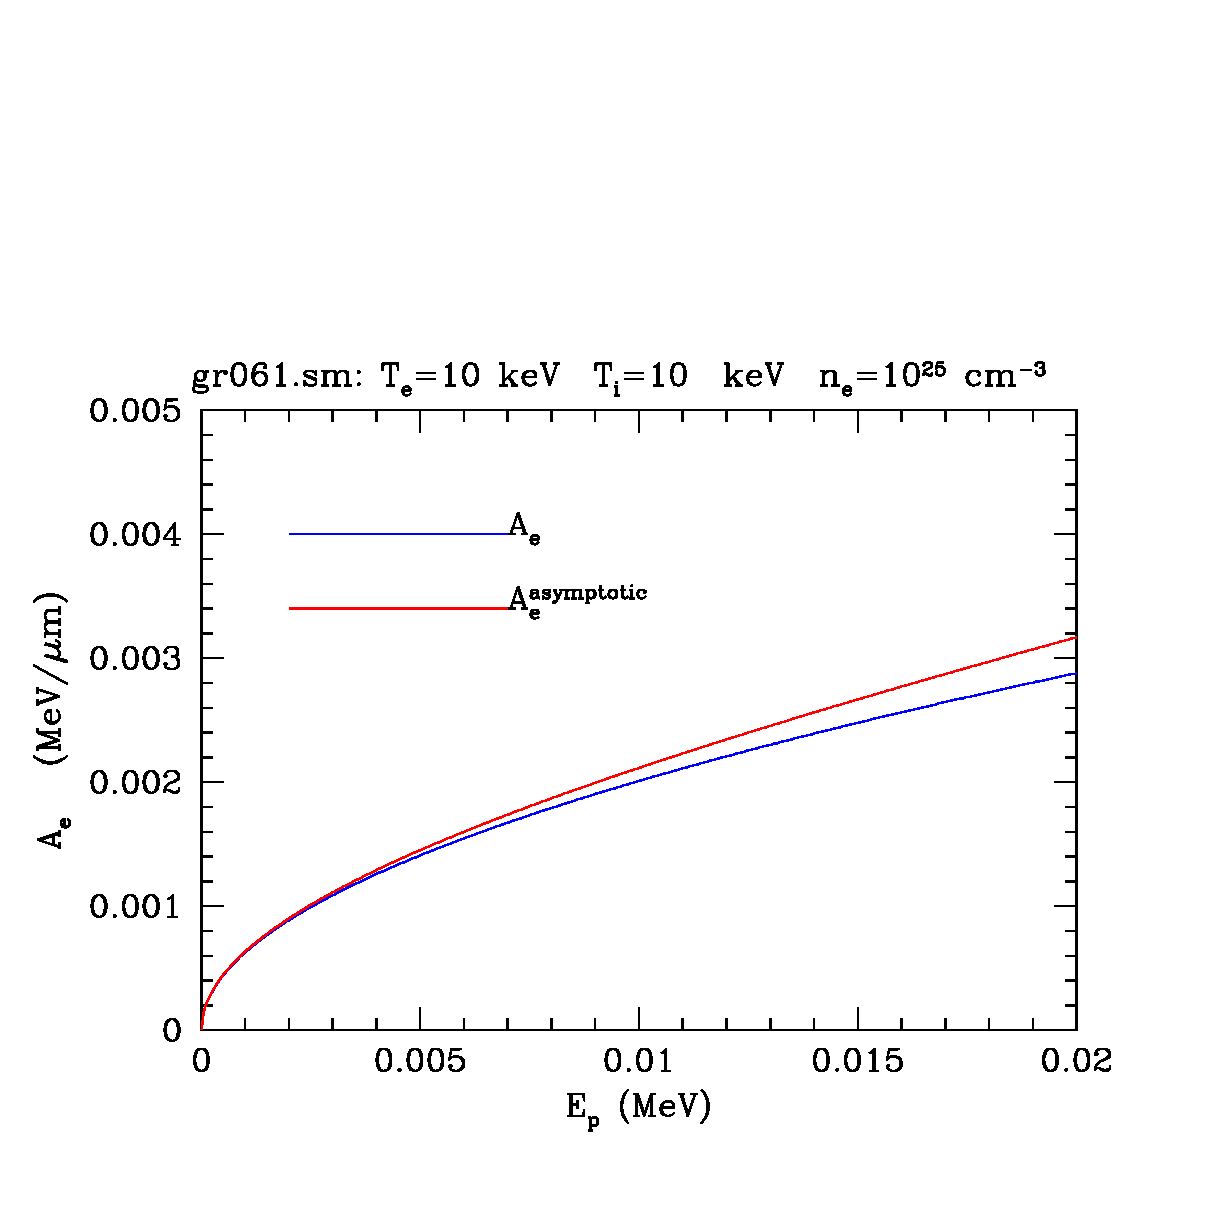
\includegraphics[scale=0.45]{gr061.eps} 
\vskip-0.8cm 
\caption{\footnoteskip  
%%
  Total asymptotic electron contribution at low energies. 
 [gr001.f90, gr061.sm,
    gr001.dat, gr001.smallE.dat, gr061.eps]
%%
}
\label{fig:gr061}
\end{figure}
%%


\pagebreak
\subsubsection{Temperatures $T_e=10\,{\rm keV}$ and $T_\smI=100\,{\rm keV}$}

%%
\vskip-2cm 
\begin{figure}[h!]
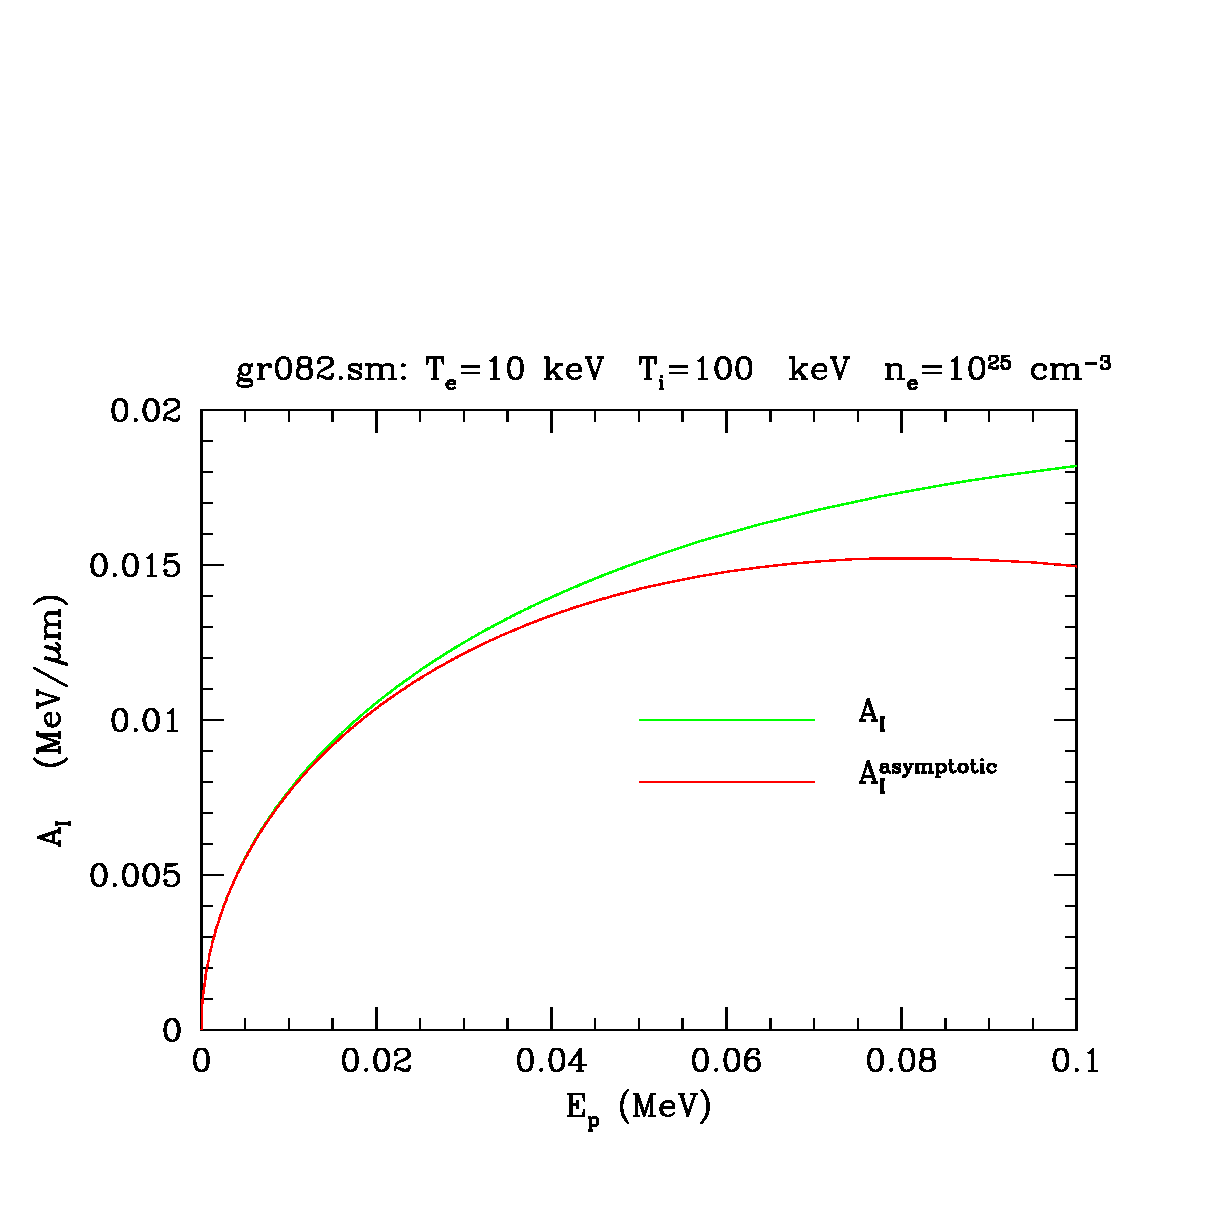
\includegraphics[scale=0.45]{gr082.eps} 
\vskip-0.8cm 
\caption{\footnoteskip  
%%
  Total asymptotic ion contribution at low energies. 
 [gr002.f90, gr082.sm, gr002.dat, gr002.smallE.dat, gr082.eps]
%%
}
\label{fig:gr082}
\end{figure}
%%

%%
\vskip-2cm 
\begin{figure}[h!]
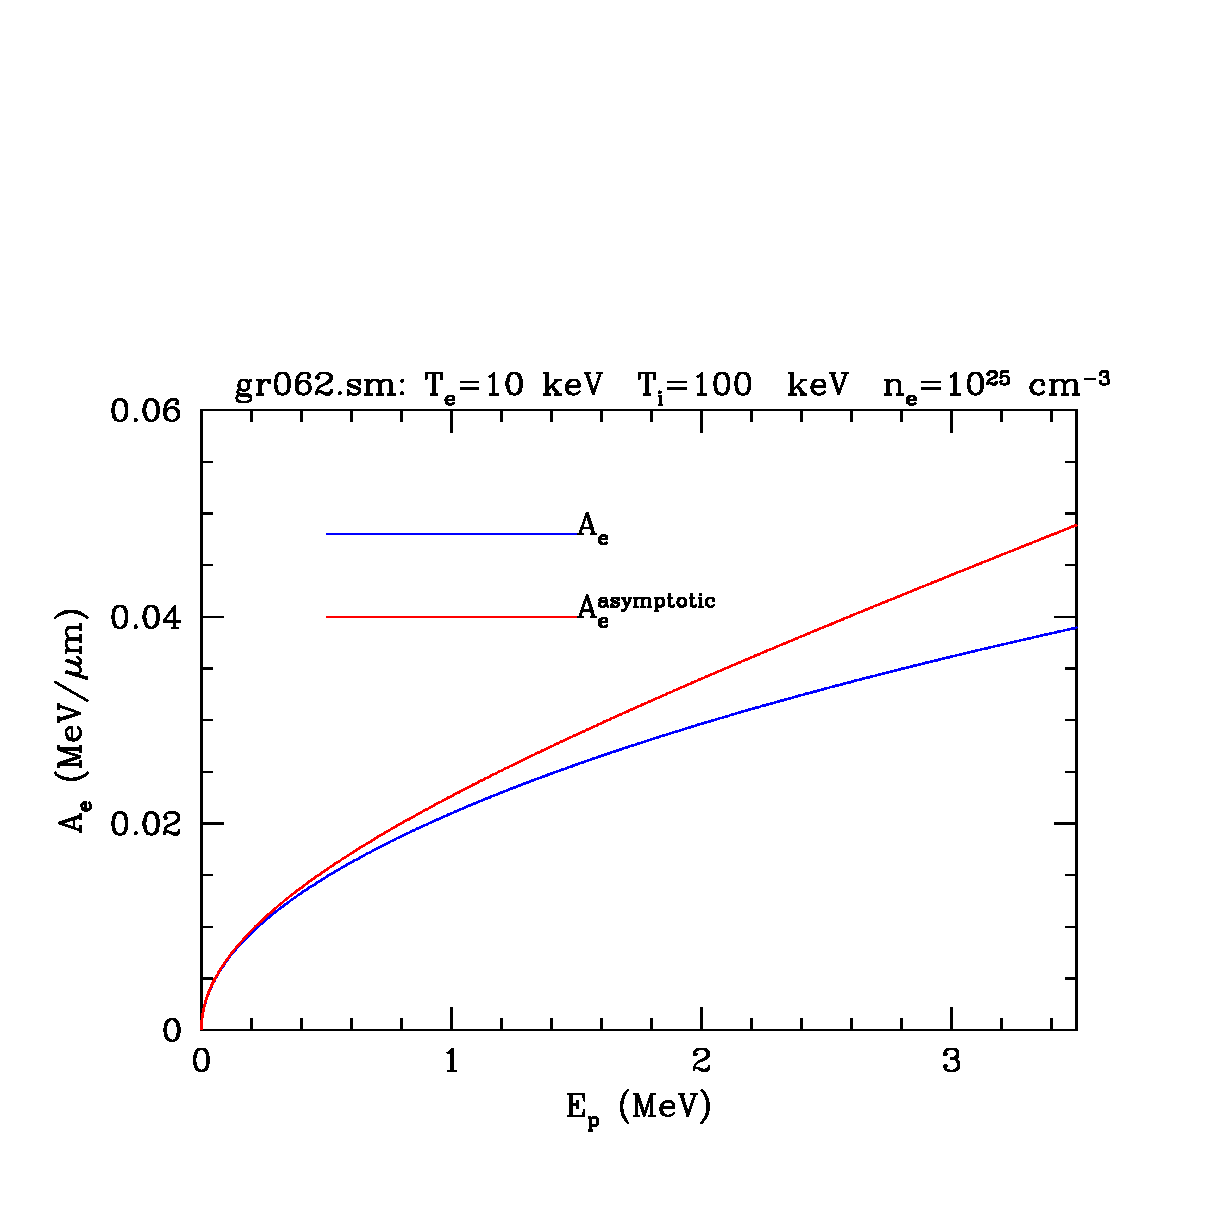
\includegraphics[scale=0.45]{gr062.eps} 
\vskip-0.8cm 
\caption{\footnoteskip  
%%
  Total asymptotic electron contribution at low energies. 
 [gr002.f90, gr062.sm, gr002.dat, gr002.smallE.dat, gr062.eps]
%%
}
\label{fig:gr062}
\end{figure}
%%


\pagebreak
\subsubsection{Temperatures $T_e=100\,{\rm keV}$ and $T_\smI=10\,{\rm
    keV}$}

%%
\vskip-2cm 
\begin{figure}[h!]
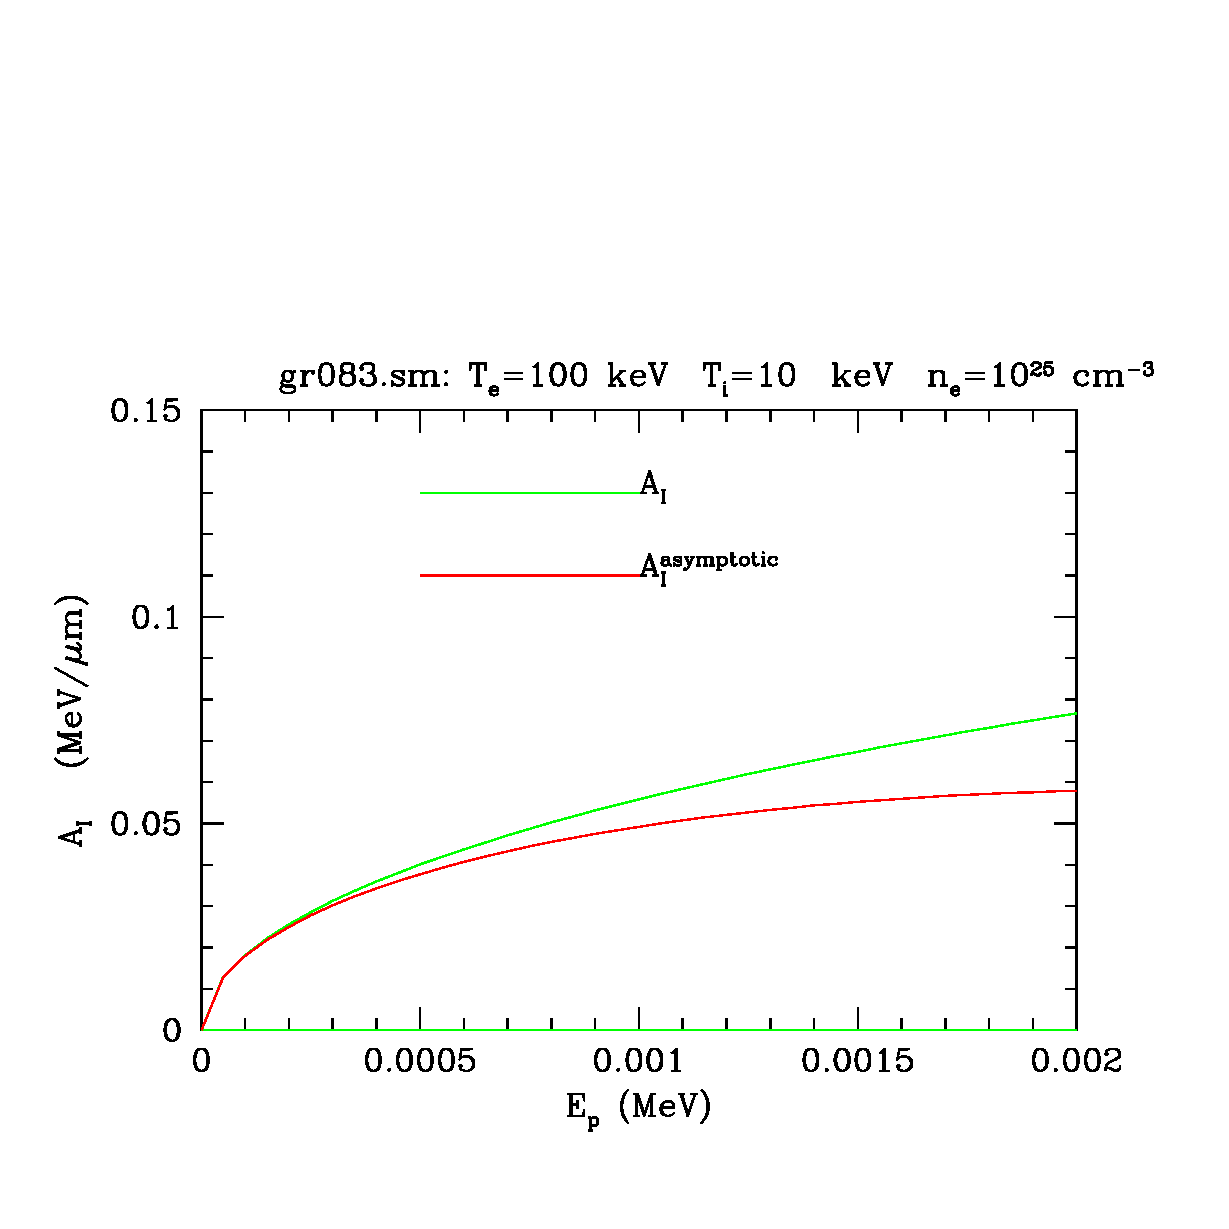
\includegraphics[scale=0.45]{gr083.eps} 
\vskip-0.8cm 
\caption{\footnoteskip  
%%
  Total asymptotic ion contribution at low energies. 
 [gr003.f90, gr083.sm, gr003.dat, gr003.smallE.dat, gr083.eps]
%%
}
\label{fig:gr083}
\end{figure}
%%

%%
\vskip-2cm 
\begin{figure}[h!]
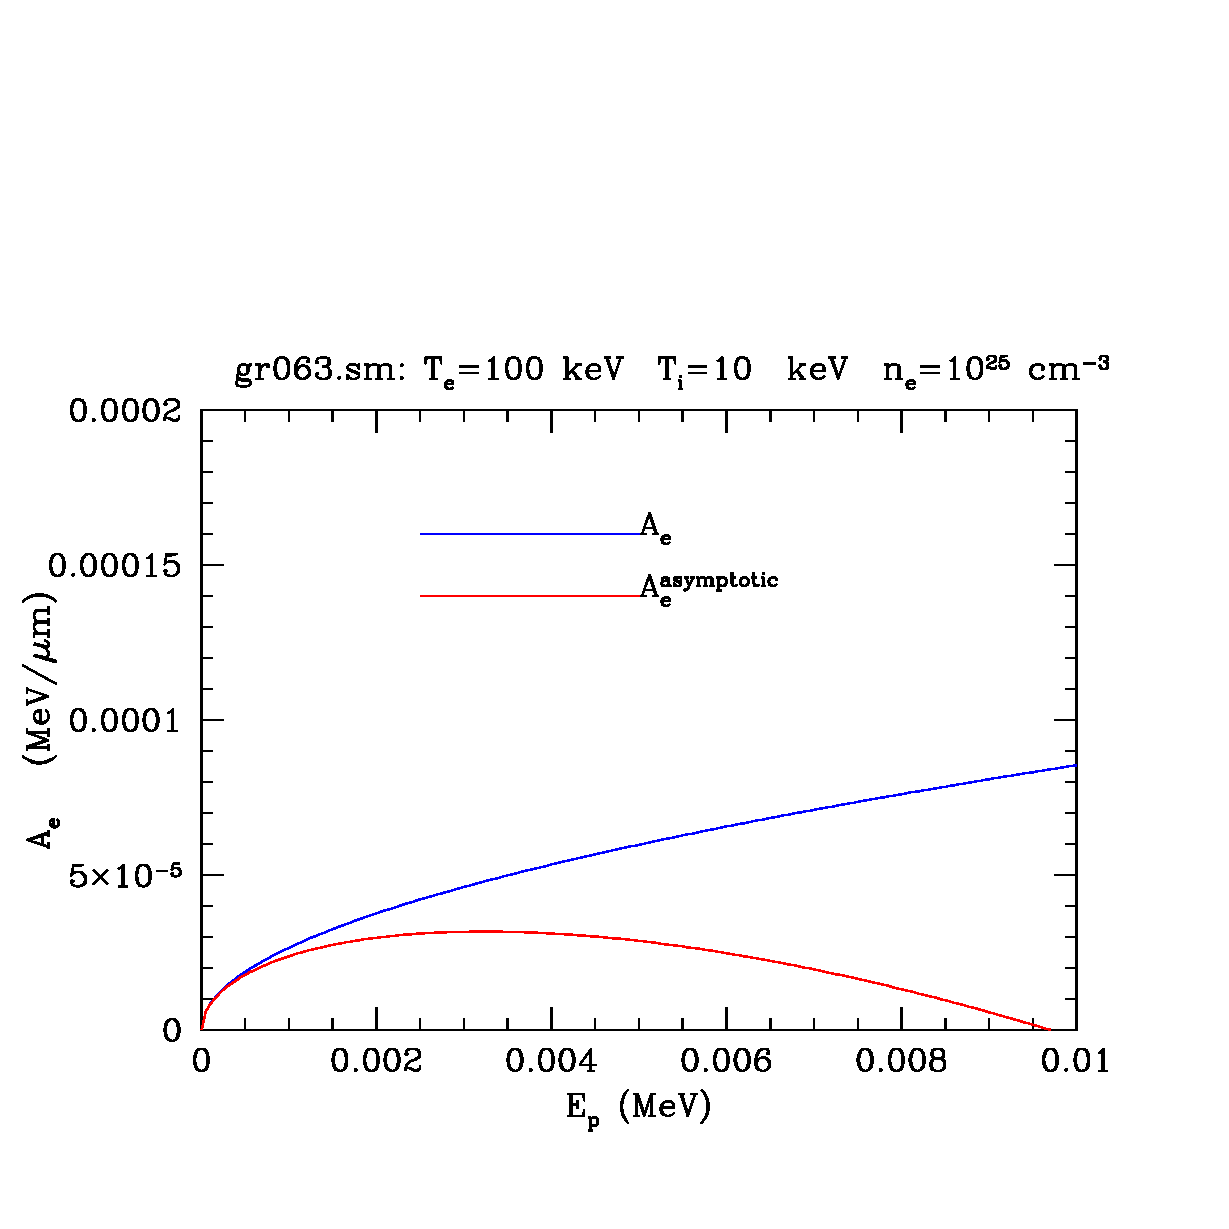
\includegraphics[scale=0.45]{gr063.eps} 
\vskip-0.8cm 
\caption{\footnoteskip  
%%
  Total asymptotic electron contribution at low energies. 
 [gr003.f90, gr063.sm, gr003.dat, gr003.smallE.dat, gr063.eps]
%%
}
\label{fig:gr063}
\end{figure}
%%



\pagebreak
\section{High Energy Asymptotic Behavior}

\subsection{Ions: Classical and Quantum}

We will look at ion contributions before looking at the electrons
(this is because there are two high energy electron regimes).  For
high energy $E \gg T$, the ion contribution to the ${\cal
A}$-coefficient becomes
%%
\begin{eqnarray}
  E_p \gg T :
  {\cal A}_\smI^\smC &=& 
  \frac{e_p^2}{4\pi}\, \frac{1}{v_p^2} \,
  {\sum}_i \omega_i^2 \left[
  -\ln\left\{\frac{e_p e_i \kappa_e}{16\pi}\, 
  \frac{2}{m_{pi} v_p^2} \right\} - \gamma - \frac{1}{2}
  \right] 
  ~~\text{[(B36) in text]}
\label{highIa}
\\[5pt]
  {\cal A}_\smI^\smQM &=& 
  \frac{e_p^2}{4\pi}\, \frac{1}{v_p^2} \,
  {\sum}_i \omega_i^2 \left[
  -\ln\left\{\frac{\hbar \kappa_e}{2 m_{pi} v_p} \right\}  - \frac{1}{2}
  \right] \ .
\label{highIb}
\end{eqnarray}
%% 
To see this, note that the classical singular ion contribution at high
energy is given by (B40) [v3.6]:
%%
\begin{eqnarray}
  && E_p \gg T ~~~ \eta_{pi} = \frac{e_p e_i}{4\pi\hbar v_p} \gg 1:
\nonumber \\[5pt]
  &&
  {\cal A}^\smC_{i,\smS} 
  = 
  -\frac{e_p^2}{4\pi}\, \frac{\omega_i^2}{v_p^2}\,
  \left[
  \ln\!\left\{ \frac{e_p \,e_i}{16\pi}\,\frac{2 \kappa_e}{m_{p i}
    v_p^2} \right\} + \gamma 
  \right]
  ~~~\text{[(B40) in text]}
%\\[5pt]
%  &&
%  {\cal A}^\smC_{e,\smS} 
%  = 
\end{eqnarray}
%%
The regular high energy asymptotic ion term is
%%
\begin{eqnarray}
  && E_p \gg T\,\ln\!\left\{ \frac{m_\smI T_e^3}{m_e T_\smI^3} \right\}
\nonumber \\[5pt]
  &&
  {\cal A}^\smC_{i,\smR} 
  =
  - \frac{e_p^2}{4\pi}\, \frac{\omega_i^2}{2 v_p^2} 
  ~~~\text{ [(B34) in text w/o sum]}
  \ .
\end{eqnarray}
%%
The asymptotic quantum piece is given by subtracting (B36) for the
singular contribution from (B42) [the singular + quantum], to give
%%
\begin{eqnarray}
  && E_p \gg T : ~~ \eta_{pi}=\frac{e_p e_i}{4\pi\hbar\,v_p}
\nonumber \\[5pt]
  &&
  {\cal A}^\smQM_i
  = 
  \frac{e_p^2}{4\pi}\,\frac{\omega_i^2}{v_p^2}\bigg[
  \ln \eta_{pi}  +\gamma \bigg] 
  ~~\text{note:}~
  \frac{e_p^2}{4\pi}\,\frac{\omega_i^2}{v_p^2}
  =
  \frac{e_p^2\, \kappa_i^2}{4\pi}\,\frac{\omega_i^2}{\kappa_i^2 v_p^2}
  =
  \frac{e_p^2\, \kappa_i^2}{4\pi}\,\frac{1}{m_i \beta_i v_p^2}
  \ .
\end{eqnarray}
%%
The algebra is:
%%
\begin{eqnarray}
  {\cal A}^\smQM_i
  &=& {\rm (B42)} - {\rm (B36)}
\\
  &=&
  \frac{e_p^2}{4\pi}\,\frac{\omega_i^2}{v_p^2}\left[
  \ln\!\left\{\frac{2 m_{pi} v_p}{\hbar \kappa_e} \right\}
  \right]
  -
  \frac{e_p^2}{4\pi}\,\frac{\omega_i^2}{v_p^2}\left[
  -\ln\!\left\{\frac{e_p e_i \kappa_e}{16\pi}\,
  \frac{2}{m_{pi} v_p^2} \right\}
  -\gamma
  \right]
\\
  &=&
  \frac{e_p^2}{4\pi}\,\frac{\omega_i^2}{v_p^2}\left[
  \ln\!\left\{\frac{2 m_{pi} v_p}{\hbar \kappa_e} \cdot
  \frac{e_p e_i \kappa_e}{16\pi}\,
  \frac{2}{m_{pi} v_p^2} \right\}
  +\gamma
  \right]
\\
  &=&
  \frac{e_p^2}{4\pi}\,\frac{\omega_i^2}{v_p^2}\left[
  \ln\!\left\{
  \frac{e_p e_i}{4\pi\, \hbar v_p}\,
  \right\}
  +\gamma
  \right] \ .
\end{eqnarray}
%%


\pagebreak
\subsubsection{Temperatures $T_e=10\,{\rm keV}$ and $T_\smI=10\,{\rm keV}$}

%%
\vskip-2cm 
\begin{figure}[h!]
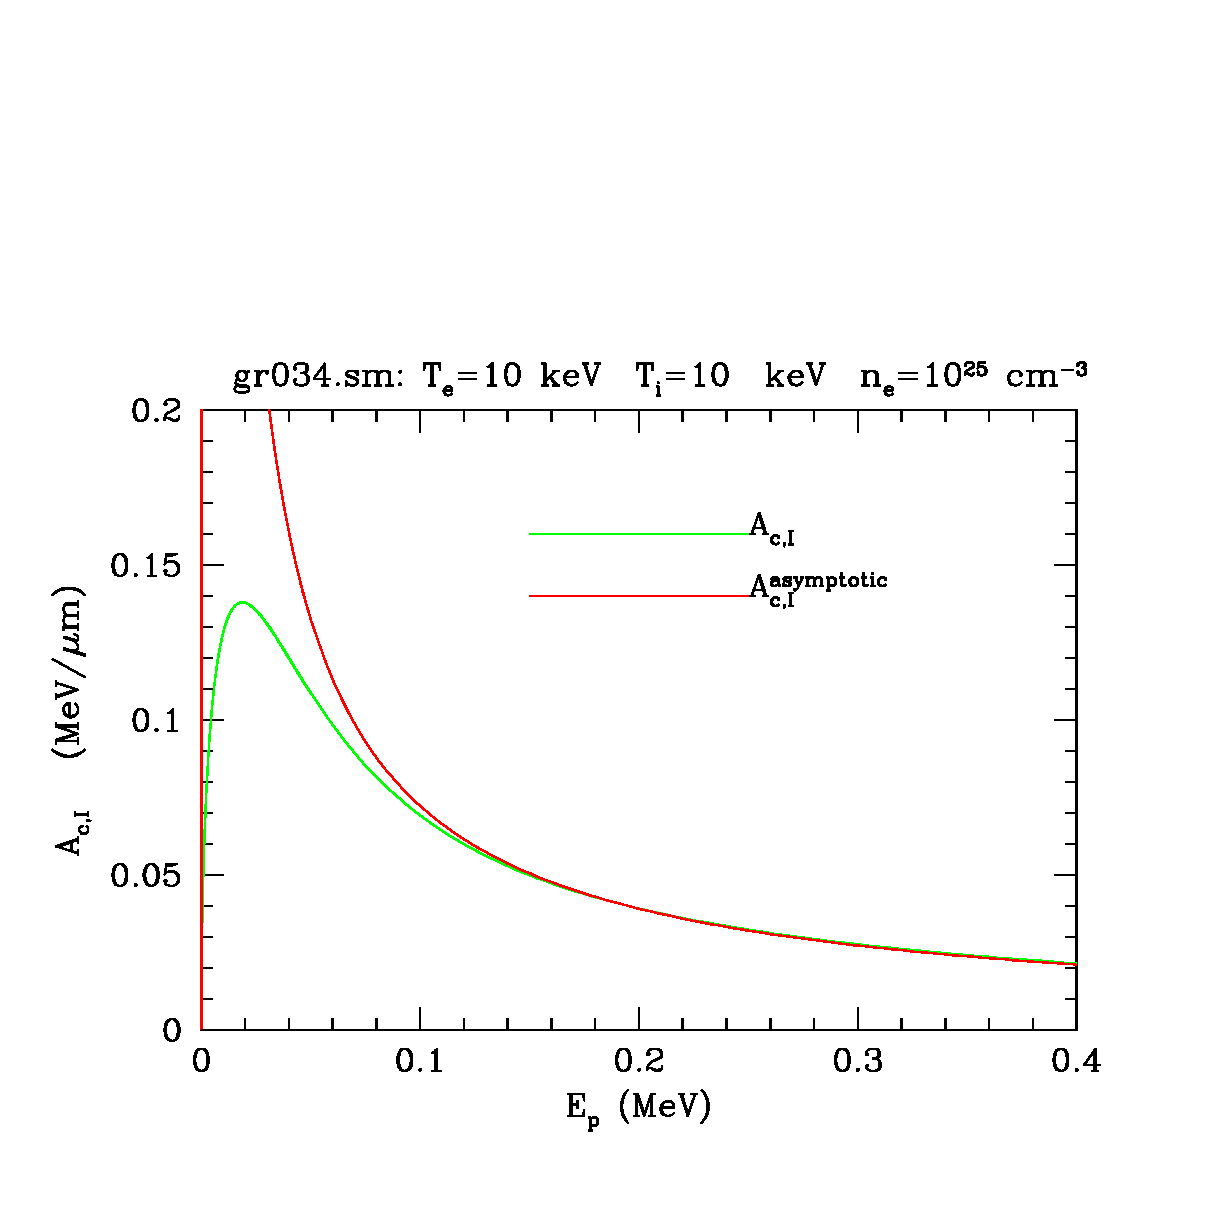
\includegraphics[scale=0.45]{gr034.eps} 
\vskip-0.8cm 
\caption{\footnoteskip  
%%
  Asymptotic classical ion contribution at high energies. [gr001.f90,
  gr034.sm, gr001.dat, gr001.highE.dat, gr034.eps]
%%
}
\label{fig:gr034}
\end{figure}
%%

%%
\vskip-2cm 
\begin{figure}[h!]
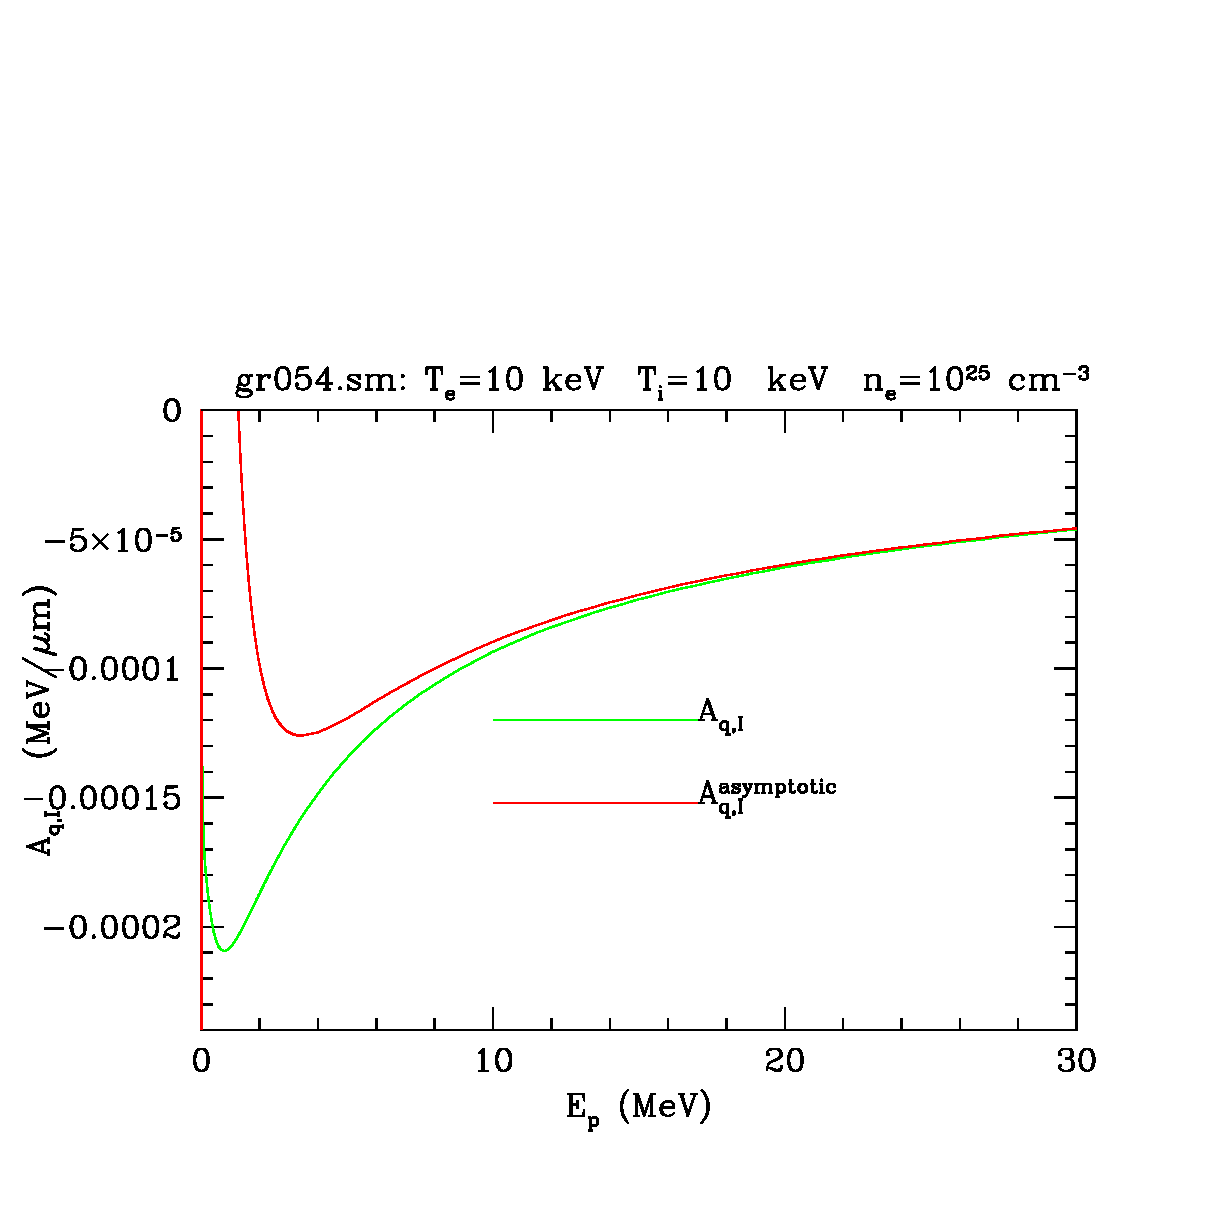
\includegraphics[scale=0.45]{gr054.eps} 
\vskip-0.8cm 
\caption{\footnoteskip  
%%
  Asymptotic quantum ion contribution at high energies. [gr001.f90,
  gr054.sm, gr001.dat, gr001.highE.dat, gr054.eps]
%%
}
\label{fig:gr054}
\end{figure}
%%

\pagebreak
\subsubsection{Temperatures $T_e=10\,{\rm keV}$ and $T_\smI=100\,{\rm keV}$}

%%
\vskip-2cm 
\begin{figure}[h!]
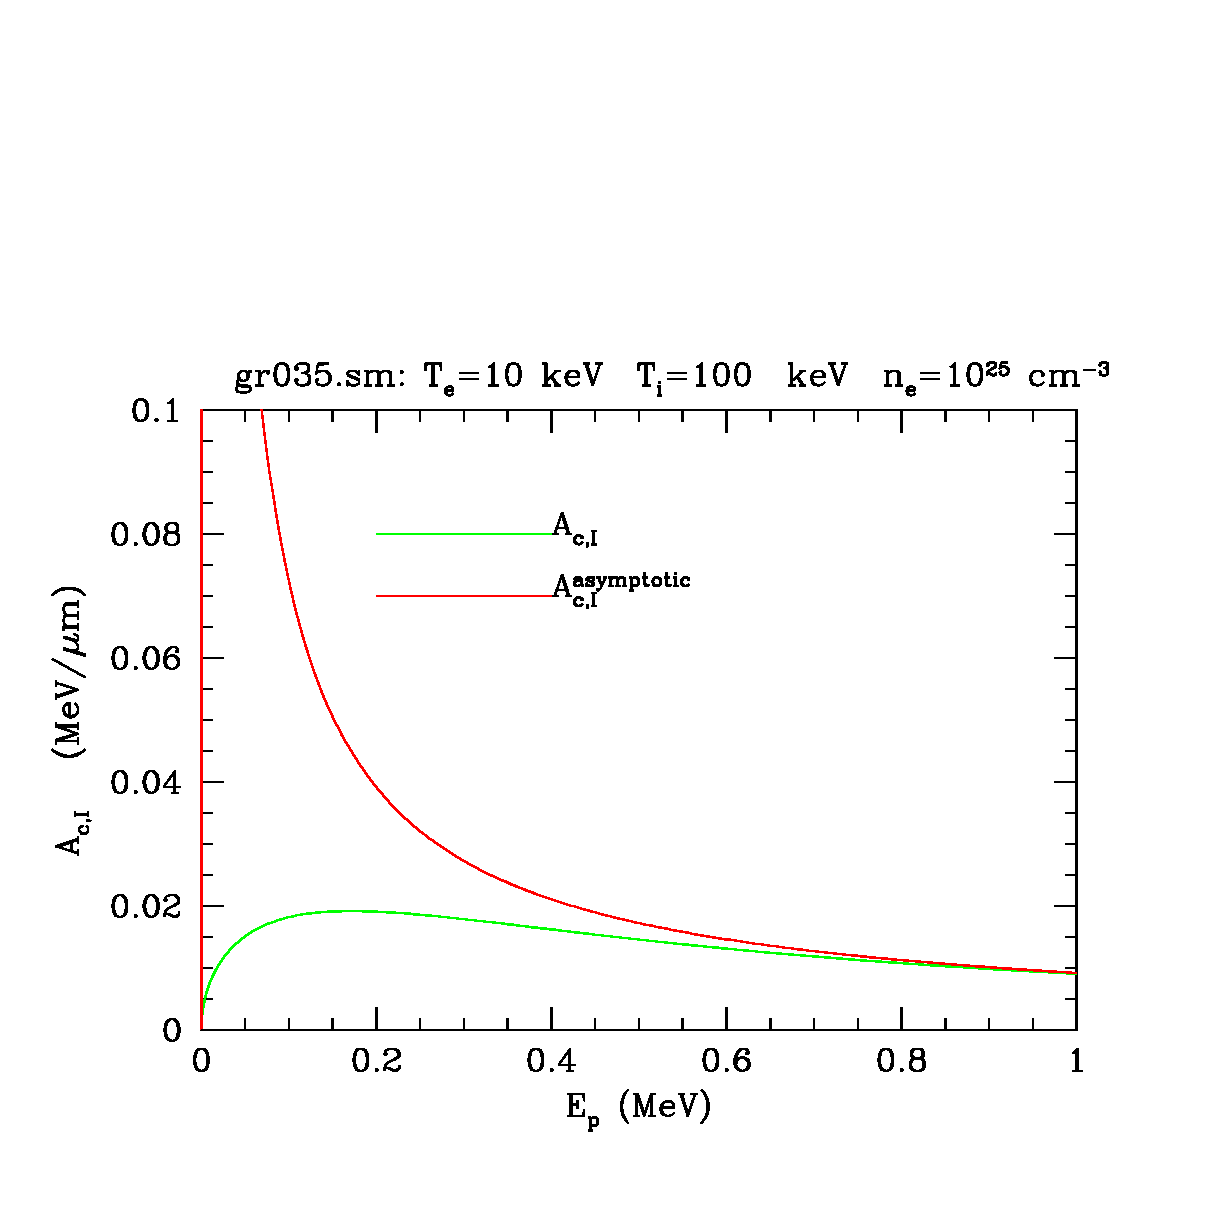
\includegraphics[scale=0.45]{gr035.eps} 
\vskip-0.8cm 
\caption{\footnoteskip  
%%
  Asymptotic classical ion contribution at high energies. [gr002.f90,
  gr035.sm, gr002.dat, gr002.highE.dat, gr035.eps]
%%
}
\label{fig:gr035}
\end{figure}
%%

%%
\vskip-2cm 
\begin{figure}[h!]
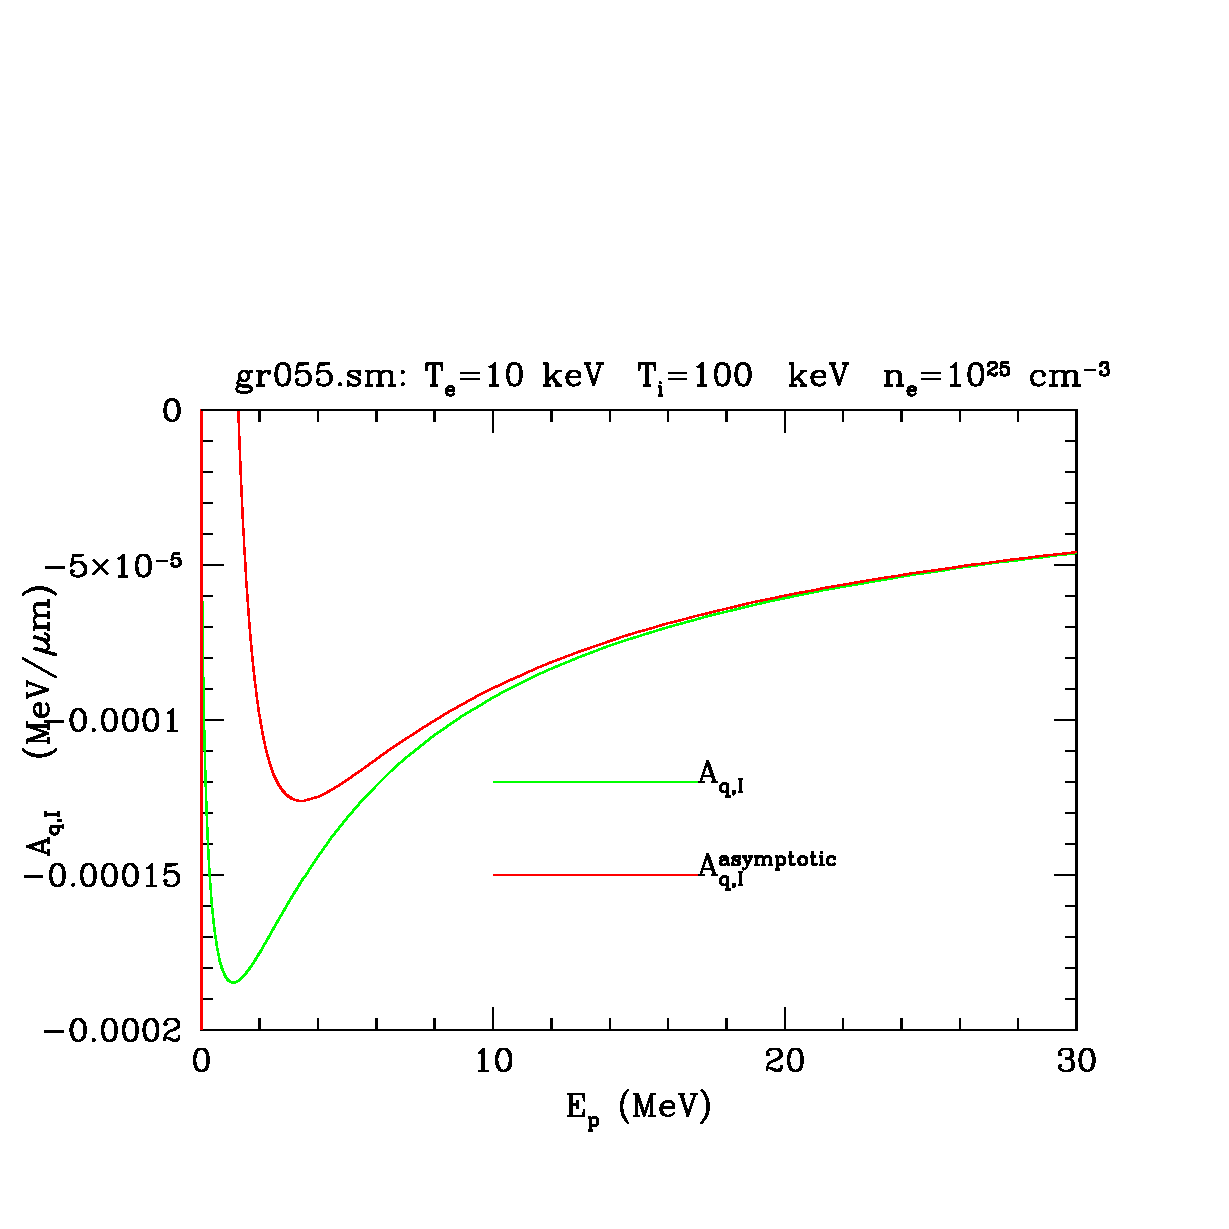
\includegraphics[scale=0.45]{gr055.eps} 
\vskip-0.8cm 
\caption{\footnoteskip  
%%
  Asymptotic quantum ion contribution at high energies. [gr002.f90,
  gr055.sm, gr002.dat, gr002.highE.dat, gr055.eps]
%%
}
\label{fig:gr055}
\end{figure}
%%

\pagebreak
\subsubsection{Temperatures $T_e=100\,{\rm keV}$ and $T_\smI=10\,{\rm keV}$}

%%
\vskip-2cm 
\begin{figure}[h!]
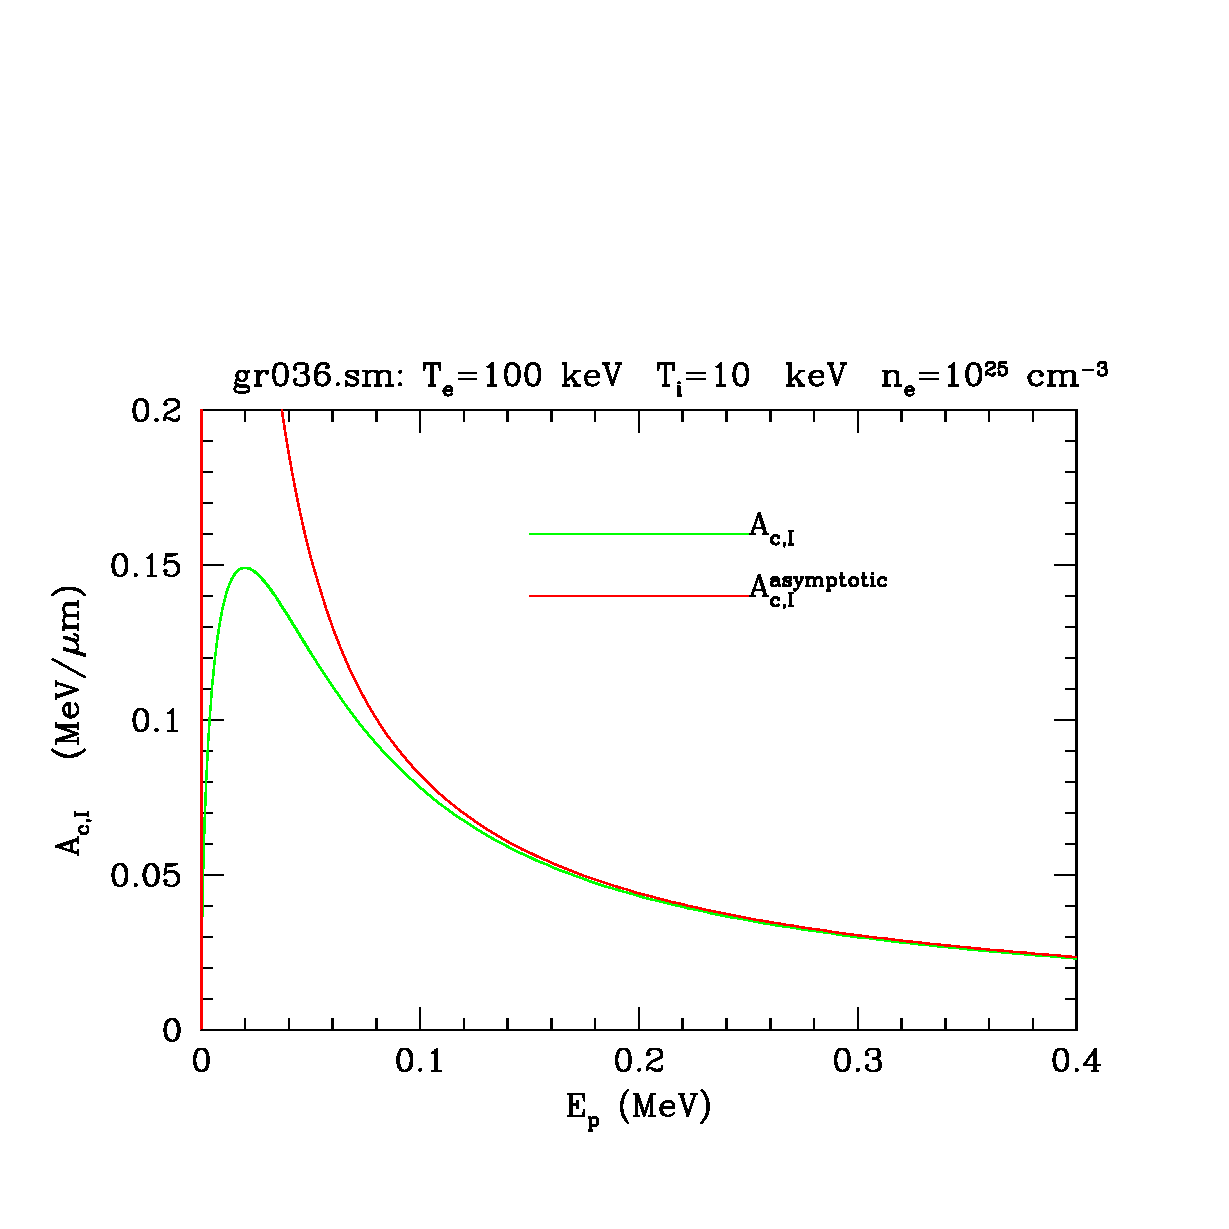
\includegraphics[scale=0.45]{gr036.eps} 
\vskip-0.8cm 
\caption{\footnoteskip  
%%
  Asymptotic classical ion contribution at high energies. [gr003.f90,
  gr036.sm, gr003.dat, gr003.highE.dat, gr036.eps]
%%
}
\label{fig:gr036}
\end{figure}
%%

%%
\vskip-2cm 
\begin{figure}[h!]
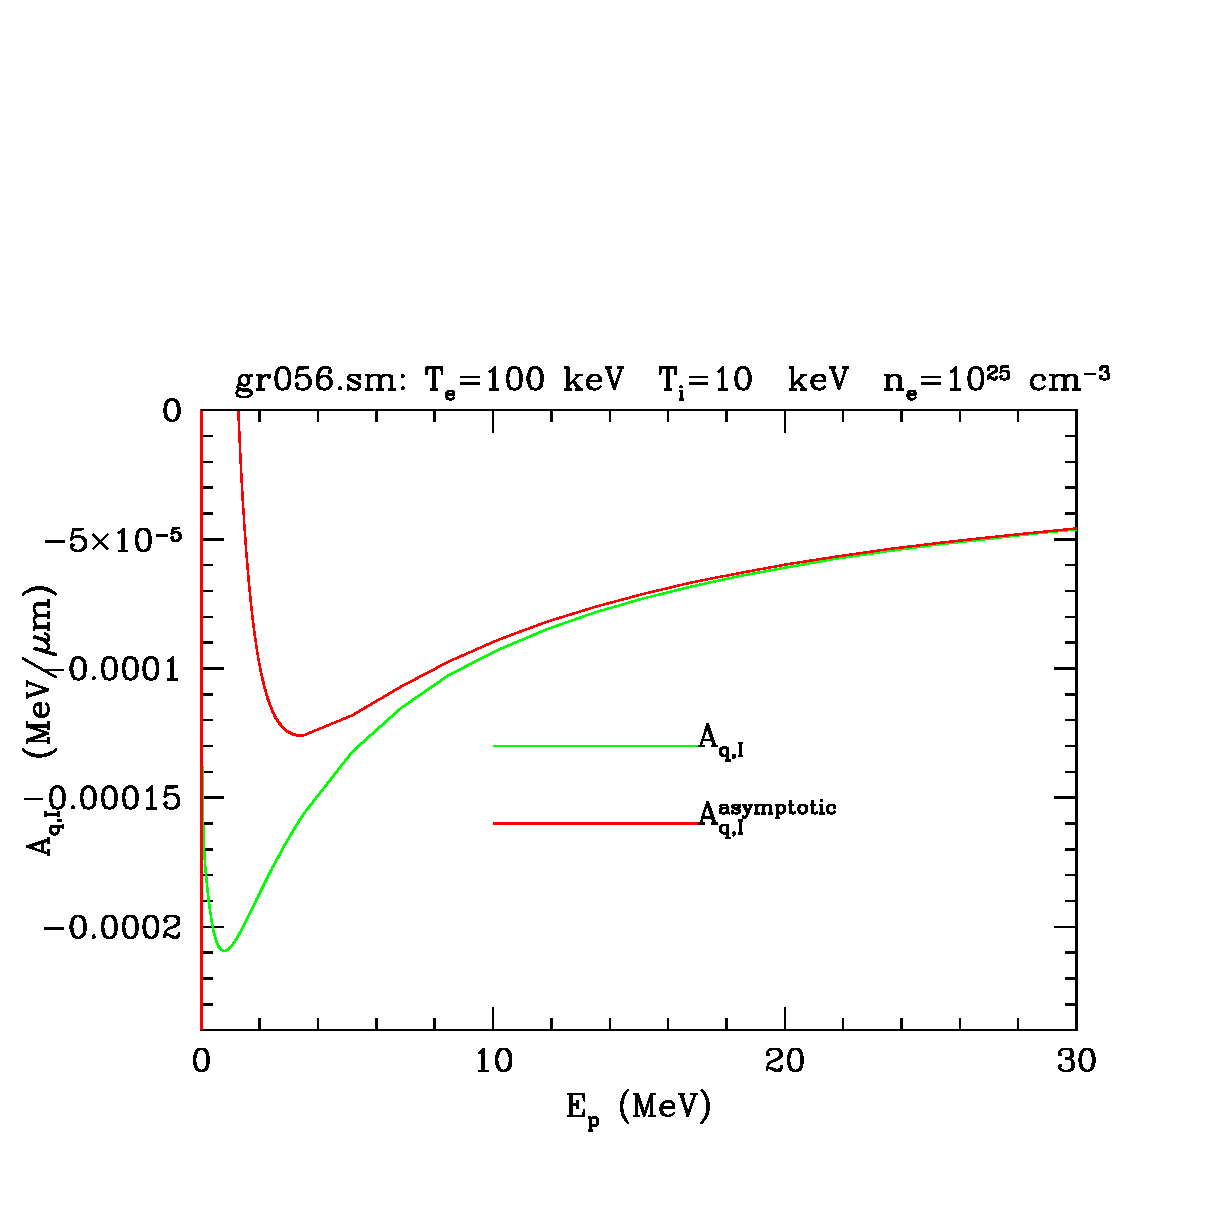
\includegraphics[scale=0.45]{gr056.eps} 
\vskip-0.8cm 
\caption{\footnoteskip  
%%
  Asymptotic quantum ion contribution at high energies. [gr003.f90,
  gr056.sm, gr003.dat, gr003.highE.dat, gr056.eps]
%%
}
\label{fig:gr056}
\end{figure}
%%

\pagebreak
\subsection{Electrons: Classical and Quantum}

The high energy electron regime is broken into two widely separated
scales, one given by $T$ and the other by $m_\smI T/m_e$. In the 
high-intermediate energy regime, 
%%
\begin{eqnarray}
  && \hskip-1.5cm 
  \frac{m_\smI}{m_e}\,T \gg E_p \gg T : 
  ~~~\text{DT plasma at 10\,keV $\Rightarrow$ $\frac{m_{\smI \,,\,{\rm
  av}}}{m_e}\, T = \frac{2.5\,{\rm GeV}}{10\,{\rm keV}}=2.5\,{\rm MeV}$. }
\nonumber
\\[3pt]
  {\cal A}_{e, \smR}^\smLT 
  &=& 
  -\frac{e_p^2\, \kappa_e^2}{4\pi}\, 
  \left(\frac{\beta_e m_e}{2\pi} \right)^{1/2}
  \frac{v_p}{3}
  \left[ \ln\left\{ \frac{\kappa_e^2}{K^2}\right\}+1 \right]
  ~~~\text{[ (B51) in text]} 
\label{Aea}
\\[10pt]
  {\cal A}_{e, \,\smS}^\smC  + {\cal A}_e^\smQM
  &=&
  \frac{e_p^2\, \kappa_e^2}{4\pi}\, 
  \left(\frac{\beta_e m_e}{2\pi} \right)^{1/2}
  \frac{v_p}{3}
  \left[ \ln\left\{ \frac{8 T_e m_{pe}^2}{m_e \hbar^2 K^2}\right\} - \gamma \right]
  ~~~\text{[ (B55) in text]}  
\label{Aeb}
\\[10pt]
  {\cal A}_e &=& 
  {\cal A}_{e, \smR}^\smLT + {\cal A}_{e, \,\smS}^\smC  
  + {\cal A}_e^\smQM
\nonumber
\\
  &=&
  \frac{e_p^2\, \kappa_e^2}{4\pi}\, 
  \left(\frac{\beta_e m_e}{2\pi} \right)^{1/2}
  \frac{v_p}{3}
  \left[ \ln\left\{ \frac{8 T_e m_{pe}^2}{m_e \hbar^2 \kappa_e^2}\right\} 
  - \gamma  -1\right]
  ~~~\text{[ (B56) in text]}  \ ,
\label{Aec}
\end{eqnarray}
%% 
and in the extreme high energy regime, 
%%
\begin{eqnarray}
  && \hskip-1.5cm 
  E_p \gg \frac{m_\smI}{m_e}\,T :
\nonumber
\\[5pt]
  {\cal A}_e &=& 
  \frac{e_p^2}{4\pi}\,\frac{\omega_e^2}{v_p^2}\,
  \ln\left\{\frac{2 m_{pe} v_p^2}{\hbar \omega_e} \right\}
  ~~~\text{[ (B58) in text]}  \ .
\end{eqnarray}
%% 
We now have the total electron contribution ${\cal A}_e$ in the
extreme and intermediate high energy regimes; however, I will have to
calculate ${\cal A}_e^\smQM$ later since the text does not give ${\cal
A}_{e,\,\smS}^\smC$ (as it did for the ions).  

I will use the coding notation: 
%%
\begin{eqnarray}
  a_b 
  &=&
  \frac{1}{2}\, \beta_b m_b v_p^2
  =
\frac{1}{2}\, \beta_b\, m_b c^2 \,\left( v_p^2/c^2\right)
\\[5pt]
  c_2 
  &=& 
  \left(\frac{a_e}{\pi}\right)^{1/2} 
  =
  \left( \frac{\beta_e m_e}{2\pi}\right)^{1/2}v_p
  =
  \left( \frac{\beta_e\, m_e c^2}{2\pi}\right)^{1/2} \frac{v_p}{c}
\\[5pt]
  c_1 
  &=&
  \frac{e_p^2 \, \kappa_e^2}{4\pi}
  =
  Z_p^2 \cdot \frac{e^2}{8\pi a_0} \cdot 2 a_0 \cdot \kappa_e^2
  =
  2 Z_p^2 \, B_e\, \kappa_e^2 a_0 \ .
\end{eqnarray}
%% 
For coding purposes, the extreme high energy electron contribution can
then be written,
%%
\begin{eqnarray}
  {\cal A}_e
  &=&
  c_1 \, \frac{\omega_e^2}{\kappa_e^2\,v_p^2}
  \ln\left\{ \frac{2 \,(m_{pe} c^2) v_p^2}{(\hbar c)\, c\,
  \omega_e}\right\} 
  =
  \frac{c_1}{\beta_e m_e v_p^2}
  \ln\left\{ \frac{2 \,(m_{pe} c^2) v_p^2}{(\hbar c)\, c\,
  \omega_e}\right\} 
\\
  &=&
  \frac{c_1}{2 a_e}
  \ln\left\{ \frac{2 \,(m_{pe} c^2) v_p^2}{(\hbar c)\, c\,
  \omega_e}\right\} 
  ~~~\text{(B58)} \ ,
\end{eqnarray}
%% 
and the intermediate high energy form is
%%
\begin{eqnarray}
  {\cal A}_e
  &=&
  \frac{c_1\,c_2}{3}
  \left[ \ln\left\{ \frac{8 T_e\, (m_{pe} c^2)^2}{(m_e c^2) (\hbar c)^2\, \kappa_e^2}\right\} 
  - \gamma  -1\right]
  ~~~\text{(B56)} \ .
\end{eqnarray}
%% 



\pagebreak
\subsubsection{Temperatures $T_e=10\,{\rm keV}$ and $T_\smI=10\,{\rm keV}$}

%%
%\vskip-2cm 
\begin{figure}[h!]
%\includegraphics[scale=0.45]{gr024.eps} !
%\vskip-0.8cm 
\caption{\footnoteskip  
%%
  Asymptotic classical electron contribution at high
  energies. [gr001.f90, gr024.sm, gr001.dat, 
  gr001.highE.dat, gr024.eps]
%%
}
\label{fig:gr024}
\end{figure}
%%

%%
%\vskip-2cm 
\begin{figure}[h!]
%\includegraphics[scale=0.45]{gr044.eps} !
\vskip-0.8cm 
\caption{\footnoteskip  
%%
  Asymptotic quantum electron contribution at high
  energies. [gr001.f90, gr044.sm, gr001.dat, gr001.highE.dat,
  gr044.eps]
%%
}
\label{fig:gr044}
\end{figure}
%%


\subsubsection{Temperatures $T_e=10\,{\rm keV}$ and $T_\smI=100\,{\rm keV}$}

%%
%\vskip-2cm 
\begin{figure}[h!]
%\includegraphics[scale=0.45]{gr025.eps} !
%\vskip-0.8cm 
\caption{\footnoteskip  
%%
  Asymptotic classical electron contribution at high
  energies. [gr002.f90, gr025.sm, gr002.dat, 
  gr002.highE.dat, gr025.eps]
%%
}
\label{fig:gr025}
\end{figure}
%%

%%
%\vskip-2cm 
\begin{figure}[h!]
%\includegraphics[scale=0.45]{gr045.eps} !
\vskip-0.8cm 
\caption{\footnoteskip  
%%
  Asymptotic quantum electron contribution at high
  energies. [gr002.f90, gr045.sm, gr002.dat, gr002.highE.dat,
  gr045.eps]
%%
}
\label{fig:gr045}
\end{figure}
%%


\subsubsection{Temperatures $T_e=100\,{\rm keV}$ and $T_\smI=10\,{\rm keV}$}

%%
%\vskip-2cm 
\begin{figure}[h!]
%\includegraphics[scale=0.45]{gr026.eps} !
%\vskip-0.8cm 
\caption{\footnoteskip  
%%
  Asymptotic classical electron contribution at high
  energies. [gr003.f90, gr026.sm, gr003.dat, 
  gr003.highE.dat, gr026.eps]
%%
}
\label{fig:gr026}
\end{figure}
%%

%%
%\vskip-2cm 
\begin{figure}[h!]
%\includegraphics[scale=0.45]{gr046.eps} !
\vskip-0.8cm 
\caption{\footnoteskip  
%%
  Asymptotic quantum electron contribution at high
  energies. [gr003.f90, gr046.sm, gr003.dat, gr003.highE.dat,
  gr046.eps]
%%
}
\label{fig:gr046}
\end{figure}
%%


\pagebreak
\subsection{Total Electron and Ion Contributions}

\subsubsection{Temperatures $T_e=10\,{\rm keV}$ and $T_\smI=10\,{\rm keV}$}

%%
\vskip-2cm 
\begin{figure}[h!]
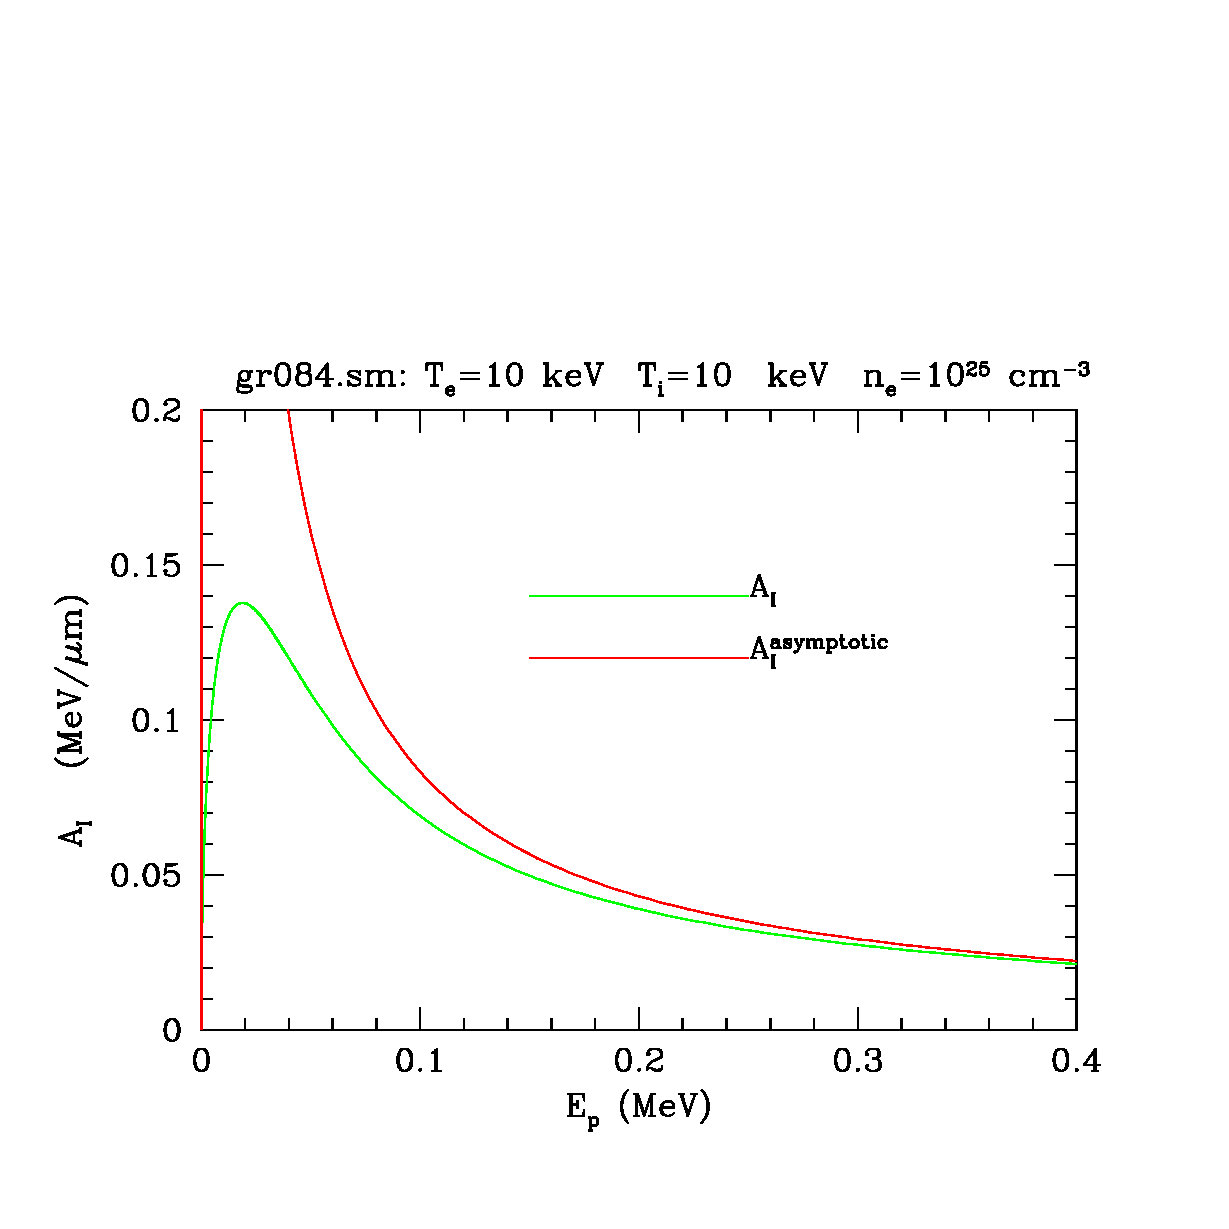
\includegraphics[scale=0.45]{gr084.eps} 
\vskip-0.8cm 
\caption{\footnoteskip  
%%
  Total asymptotic ion contribution at high energies. [gr001.f90,
  gr084.sm, gr001.dat, gr001.highE.dat, gr084.eps]
%%
}
\label{fig:gr084}
\end{figure}
%%


%%
\vskip-2cm 
\begin{figure}[h!]
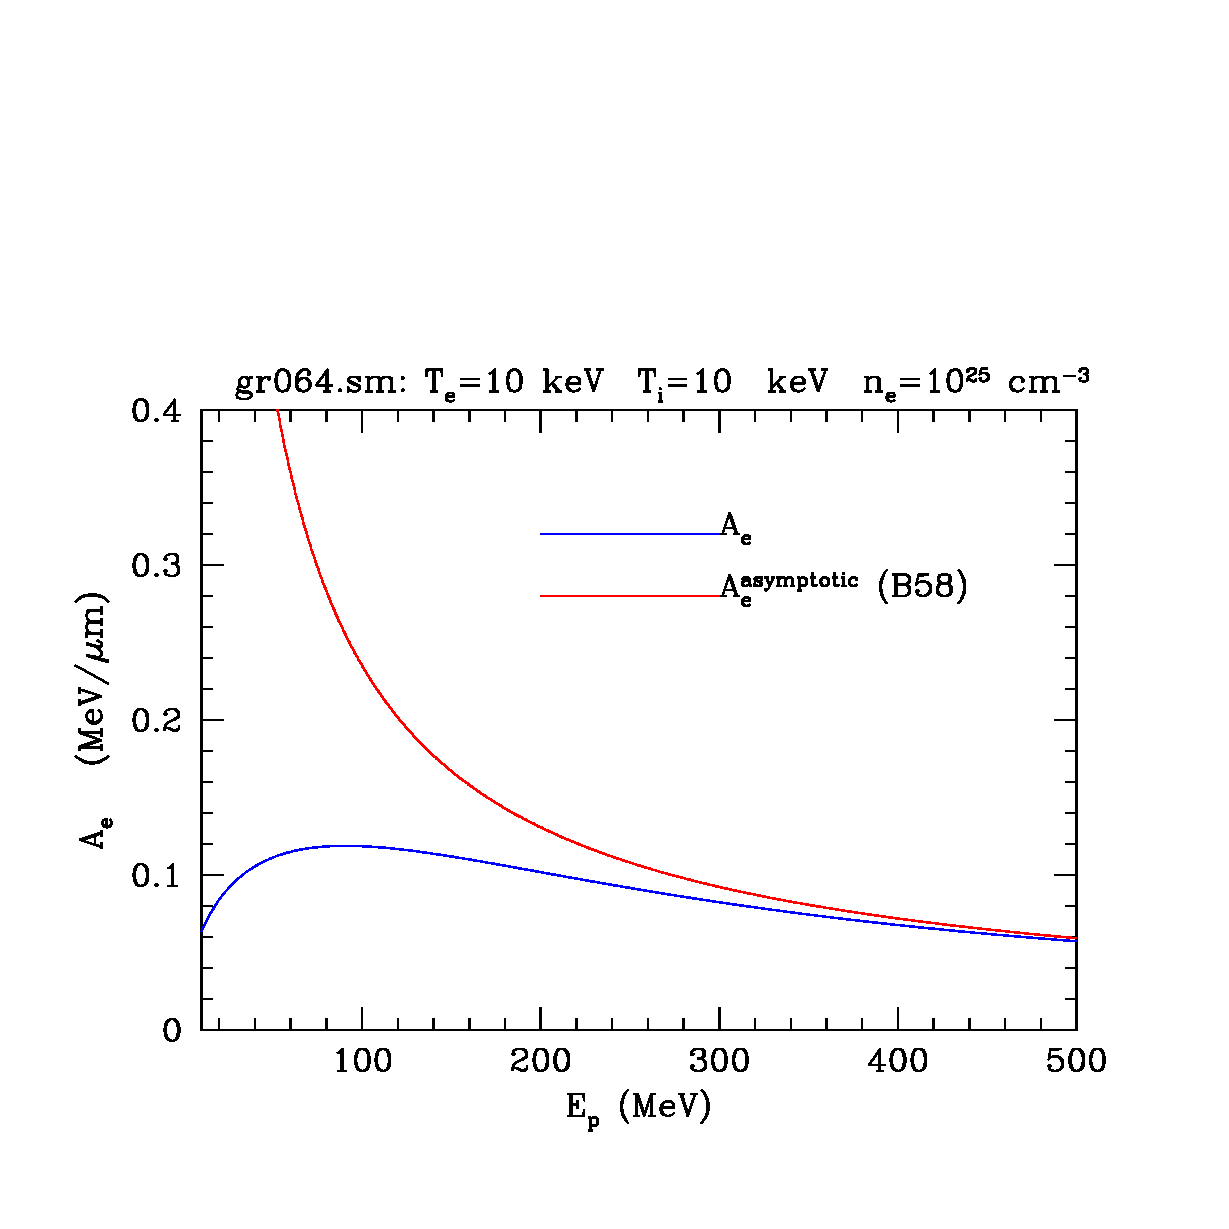
\includegraphics[scale=0.45]{gr064.eps}
\vskip-0.8cm 
\caption{\footnoteskip  
%%
  Total asymptotic electron contribution (B58) at very high
  energies. [gr001.f90, gr064.sm, gr001.dat, gr001.highEe.dat, gr064.eps]
%%
}
\label{fig:gr064}
\end{figure}
%%


\pagebreak

%%
%\vskip-2cm 
\begin{figure}[h!]
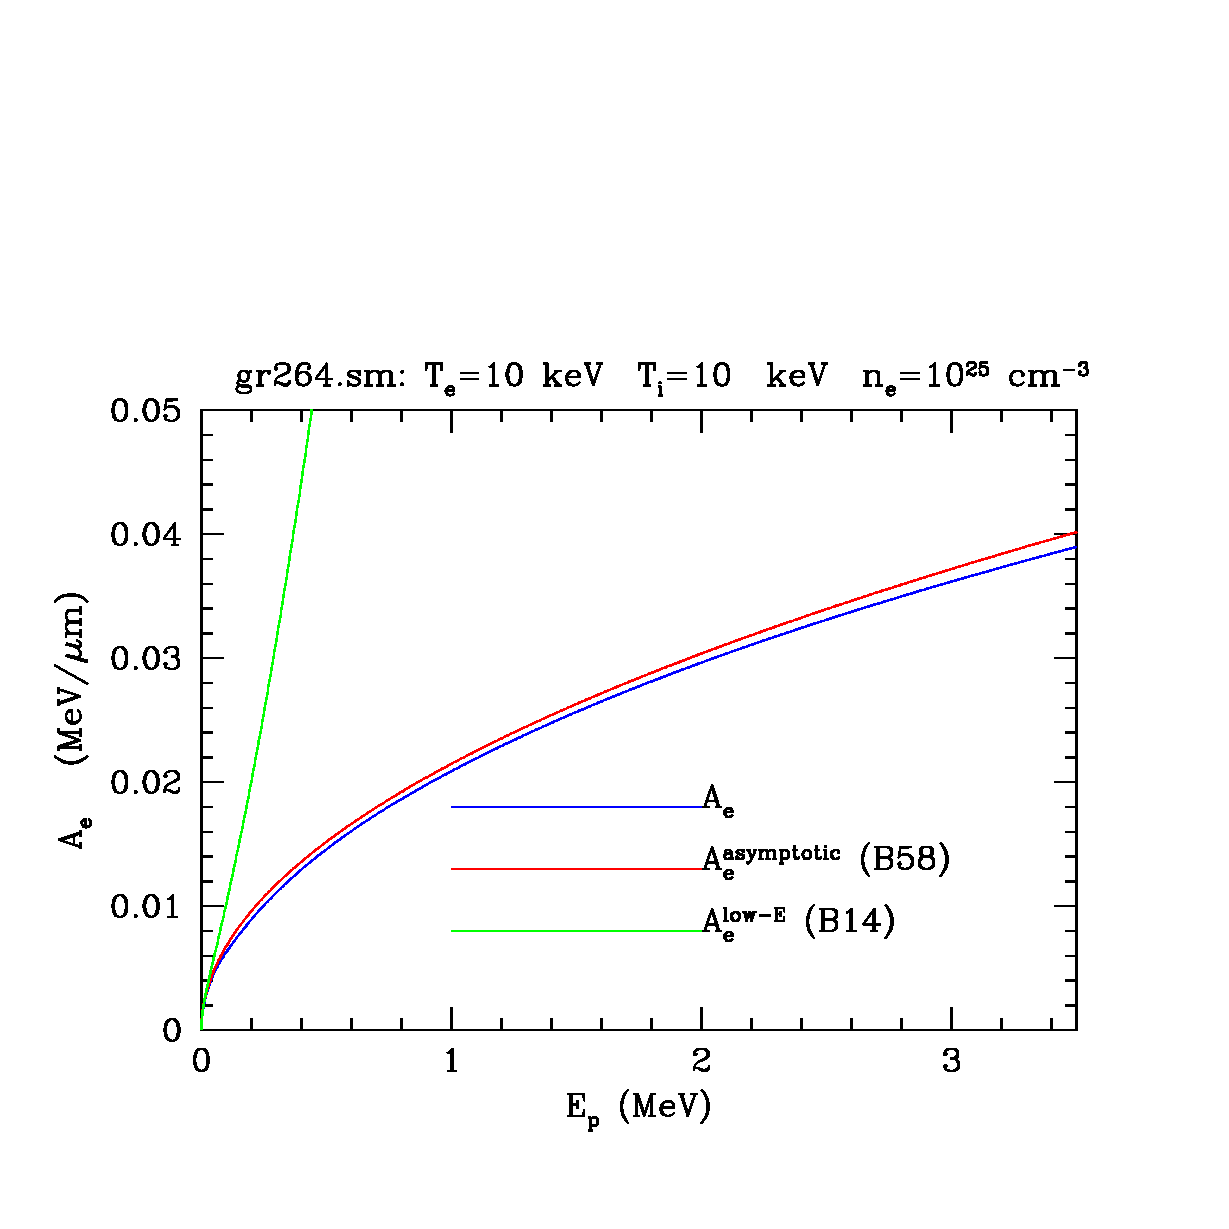
\includegraphics[scale=0.45]{gr264.eps} 
\vskip-0.8cm 
\caption{\footnoteskip  
%%
  Total asymptotic electron contribution (B56) at medium high
  energies.  [gr001.f90, gr264.sm, gr001.dat, gr001.highE.dat, gr264.eps]
%%
}
\label{fig:gr264}
\end{figure}
%%

%%
%\vskip-2cm 
\begin{figure}[h!]
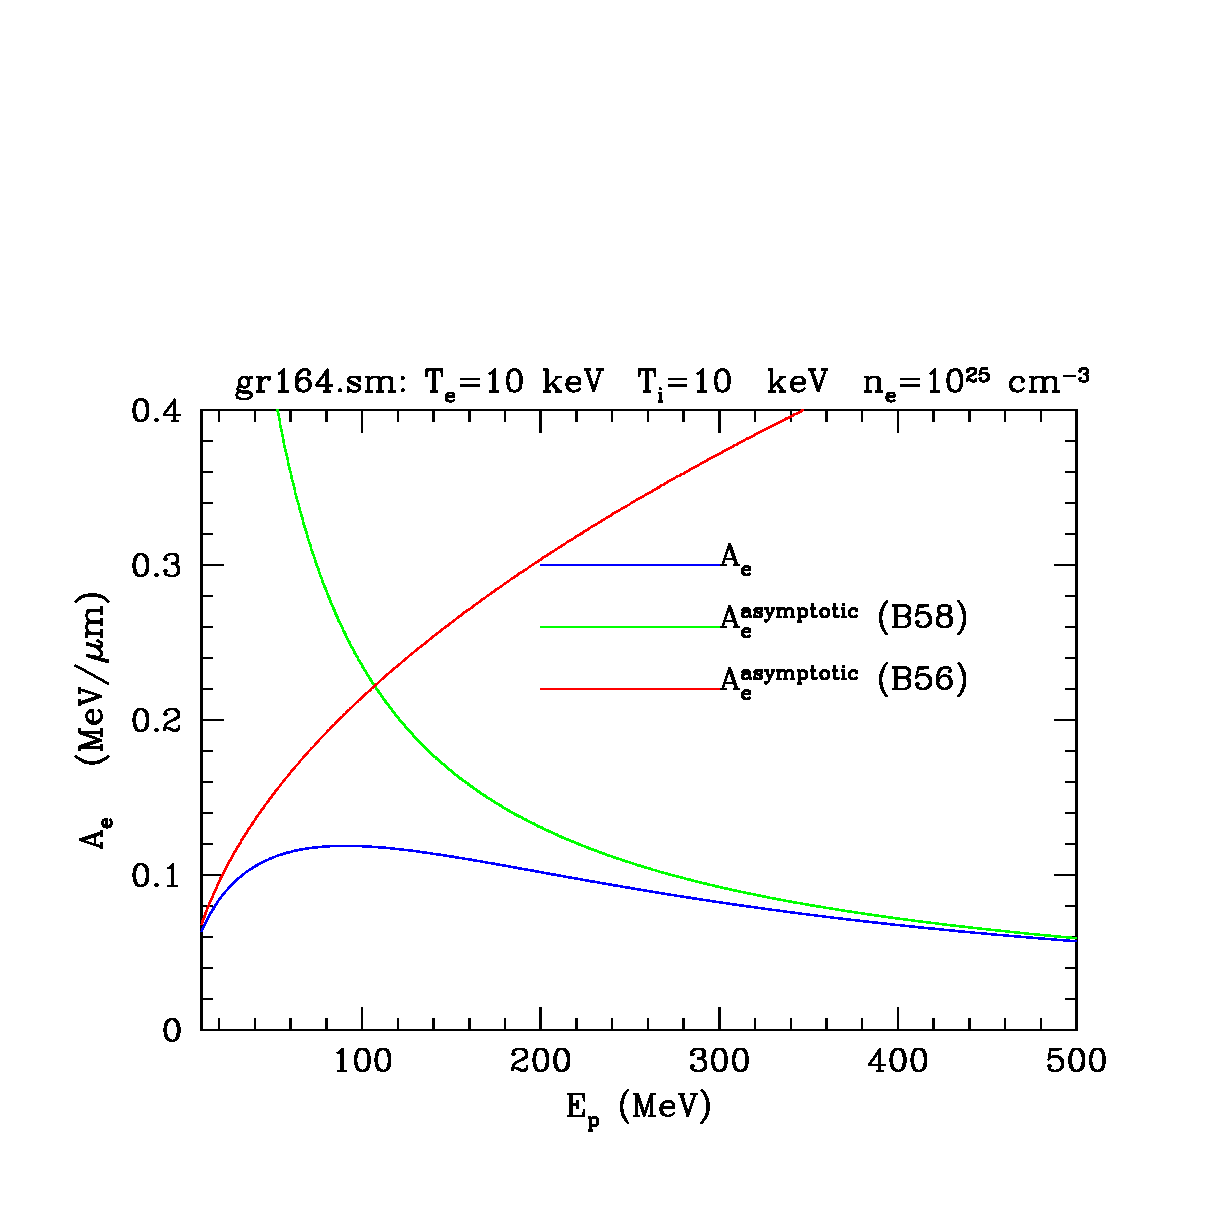
\includegraphics[scale=0.45]{gr164.eps} 
\vskip-0.8cm 
\caption{\footnoteskip  
%%
  Total asymptotic electron contribution (B56) and (B58).  [gr001.f90,
  gr164.sm, gr001.dat, gr001.highE.dat, gr001.highEe.dat, gr164.eps]
%%
}
\label{fig:gr164}
\end{figure}
%%


\vfill

\pagebreak
\subsubsection{Temperatures $T_e=10\,{\rm keV}$ and $T_\smI=100\,{\rm keV}$}

%%
\vskip-2cm 
\begin{figure}[h!]
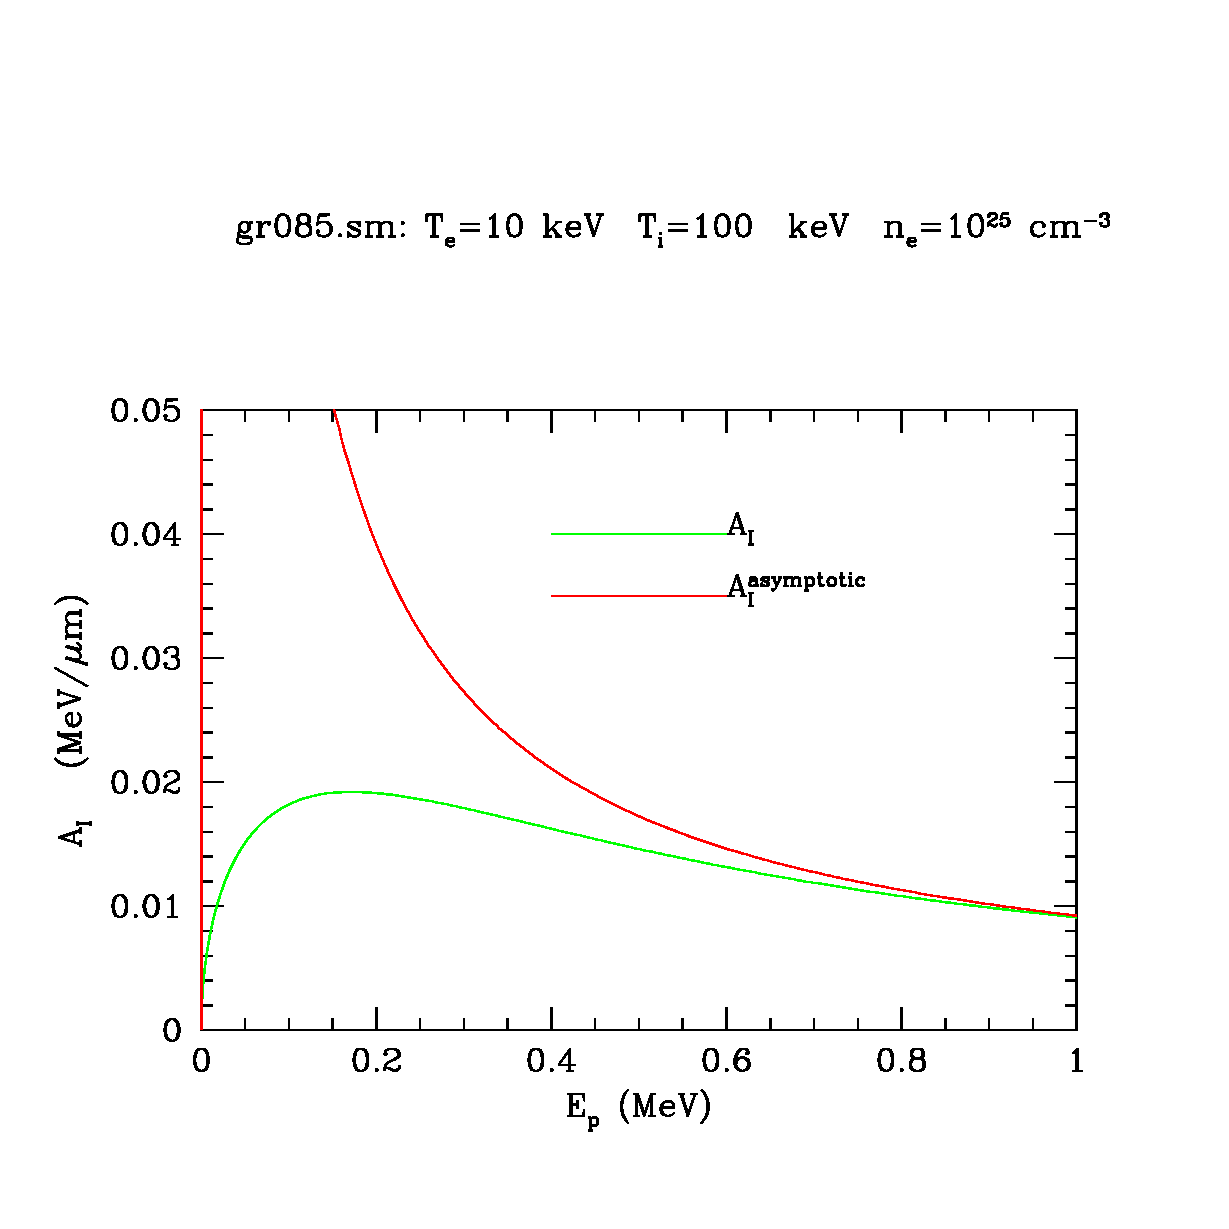
\includegraphics[scale=0.45]{gr085.eps} 
\vskip-0.8cm 
\caption{\footnoteskip  
%%
  Total asymptotic ion contribution at high energies. [gr002.f90,
  gr085.sm, gr002.dat, gr002.highE.dat, gr085.eps]
%%
}
\label{fig:gr085}
\end{figure}
%%


%%
\vskip-2cm 
\begin{figure}[h!]
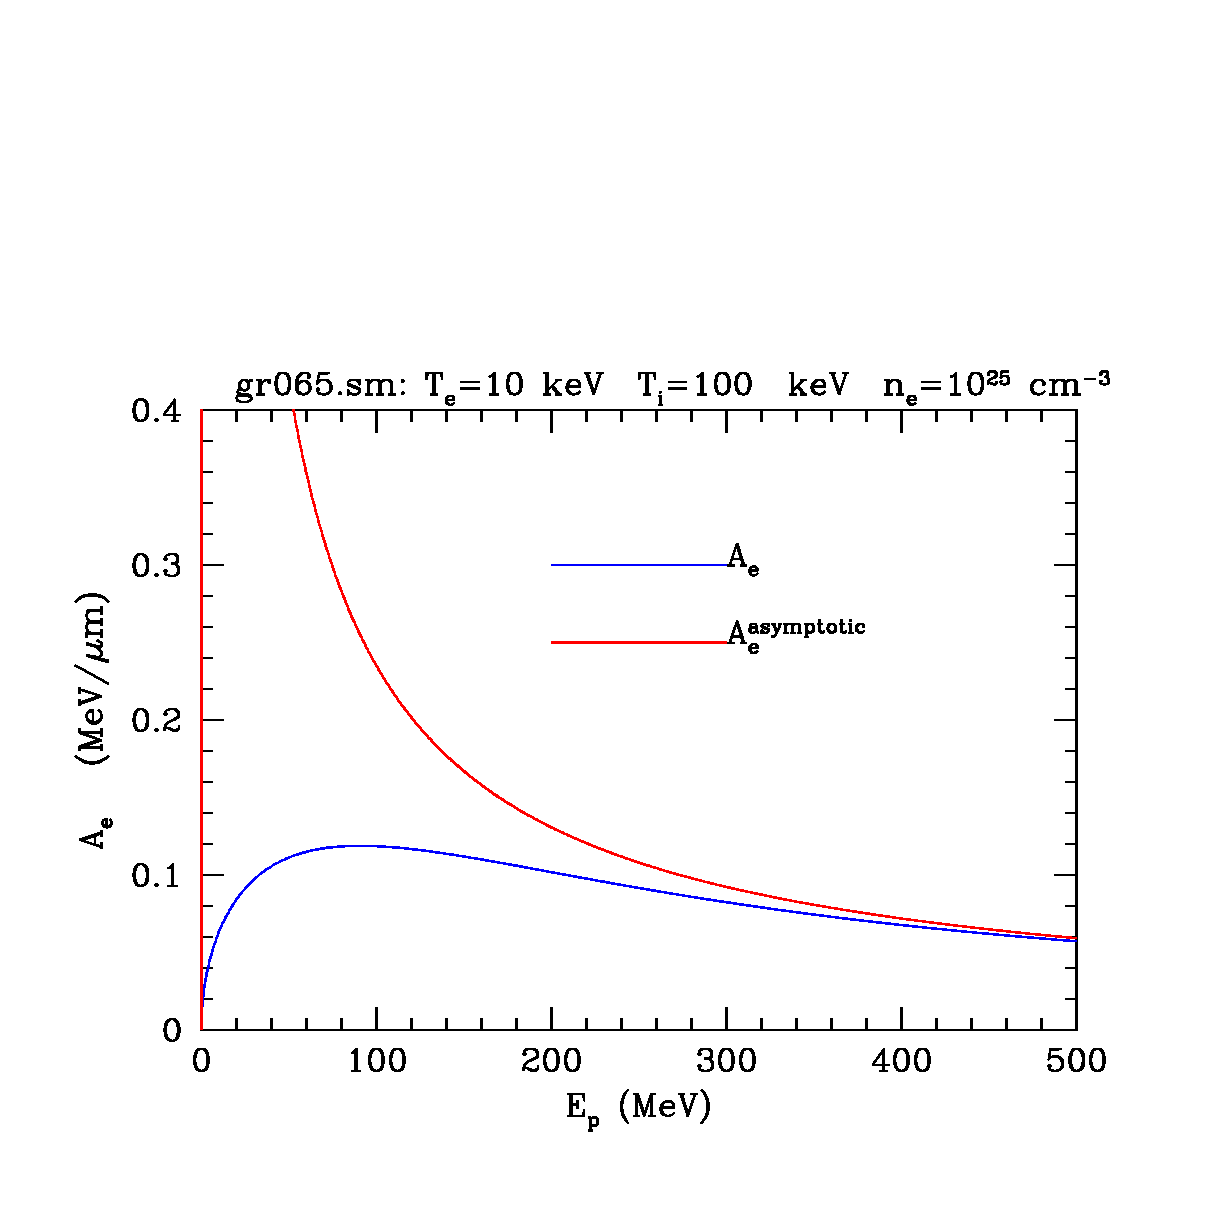
\includegraphics[scale=0.45]{gr065.eps}
\vskip-0.8cm 
\caption{\footnoteskip  
%%
  Total asymptotic electron contribution (B58) at very high
  energies. [gr002.f90, gr065.sm, gr002.dat,
  gr002.highE.dat, gr065.eps]
%%
}
\label{fig:gr065}
\end{figure}
%%


\pagebreak

%%
\vskip-2cm 
\begin{figure}[h!]
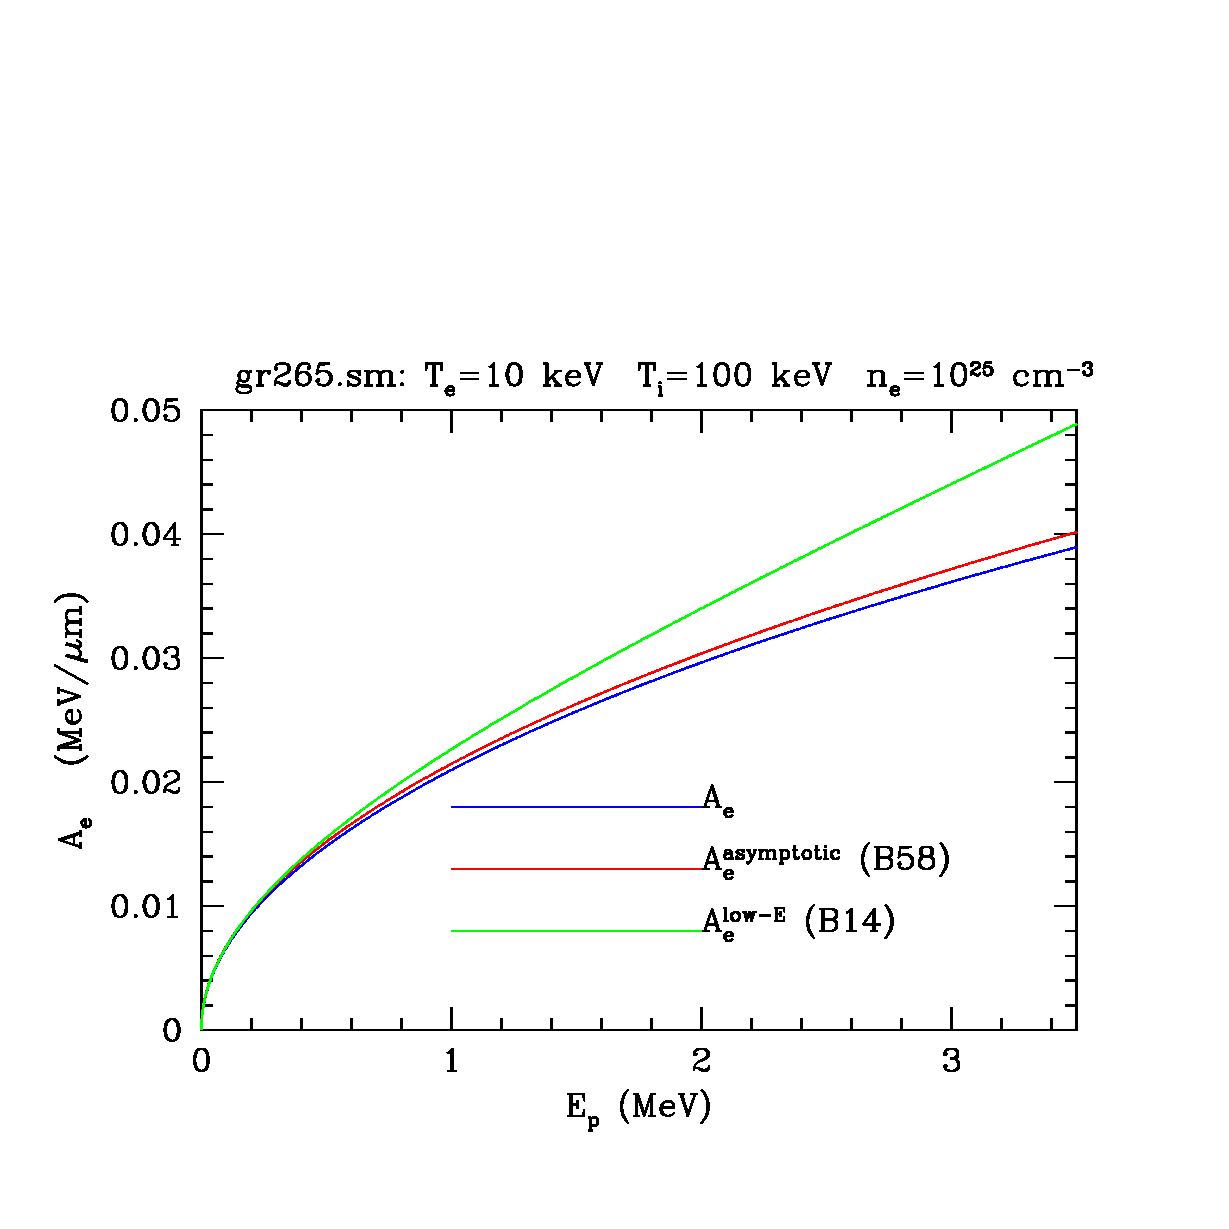
\includegraphics[scale=0.45]{gr265.eps} 
\vskip-0.8cm 
\caption{\footnoteskip  
%%
  Total asymptotic electron contribution (B56) at medium high
  energies. [gr002.f90, gr265.sm, gr002.dat, gr002.highE.dat, gr265.eps]
%%
}
\label{fig:gr265}
\end{figure}
%%

%%
\vskip-2cm 
\begin{figure}[h!]
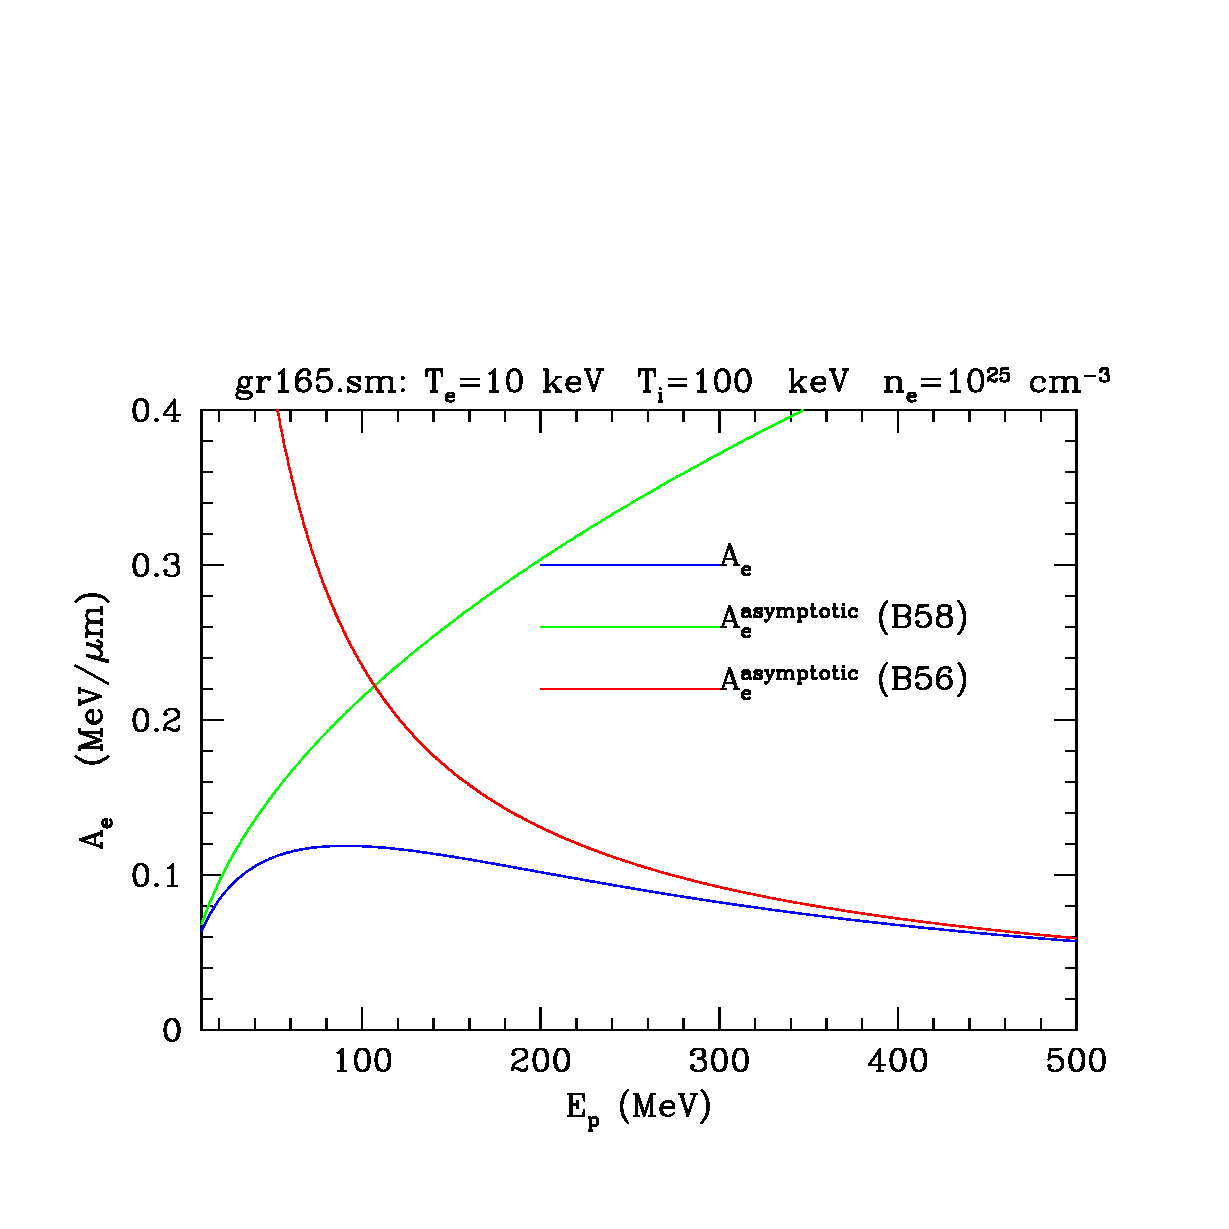
\includegraphics[scale=0.45]{gr165.eps} 
\vskip-0.8cm 
\caption{\footnoteskip  
%%
  Total asymptotic electron contribution (B56) and (B58).  [gr002.f90,
  gr165.sm, gr002.dat, gr002.highE.dat, gr002.highEe.dat, gr165.eps]
%%
}
\label{fig:gr165}
\end{figure}
%%




\pagebreak
\subsubsection{Temperatures $T_e=100\,{\rm keV}$ and $T_\smI=10\,{\rm keV}$}

%%
\vskip-2cm 
\begin{figure}[h!]
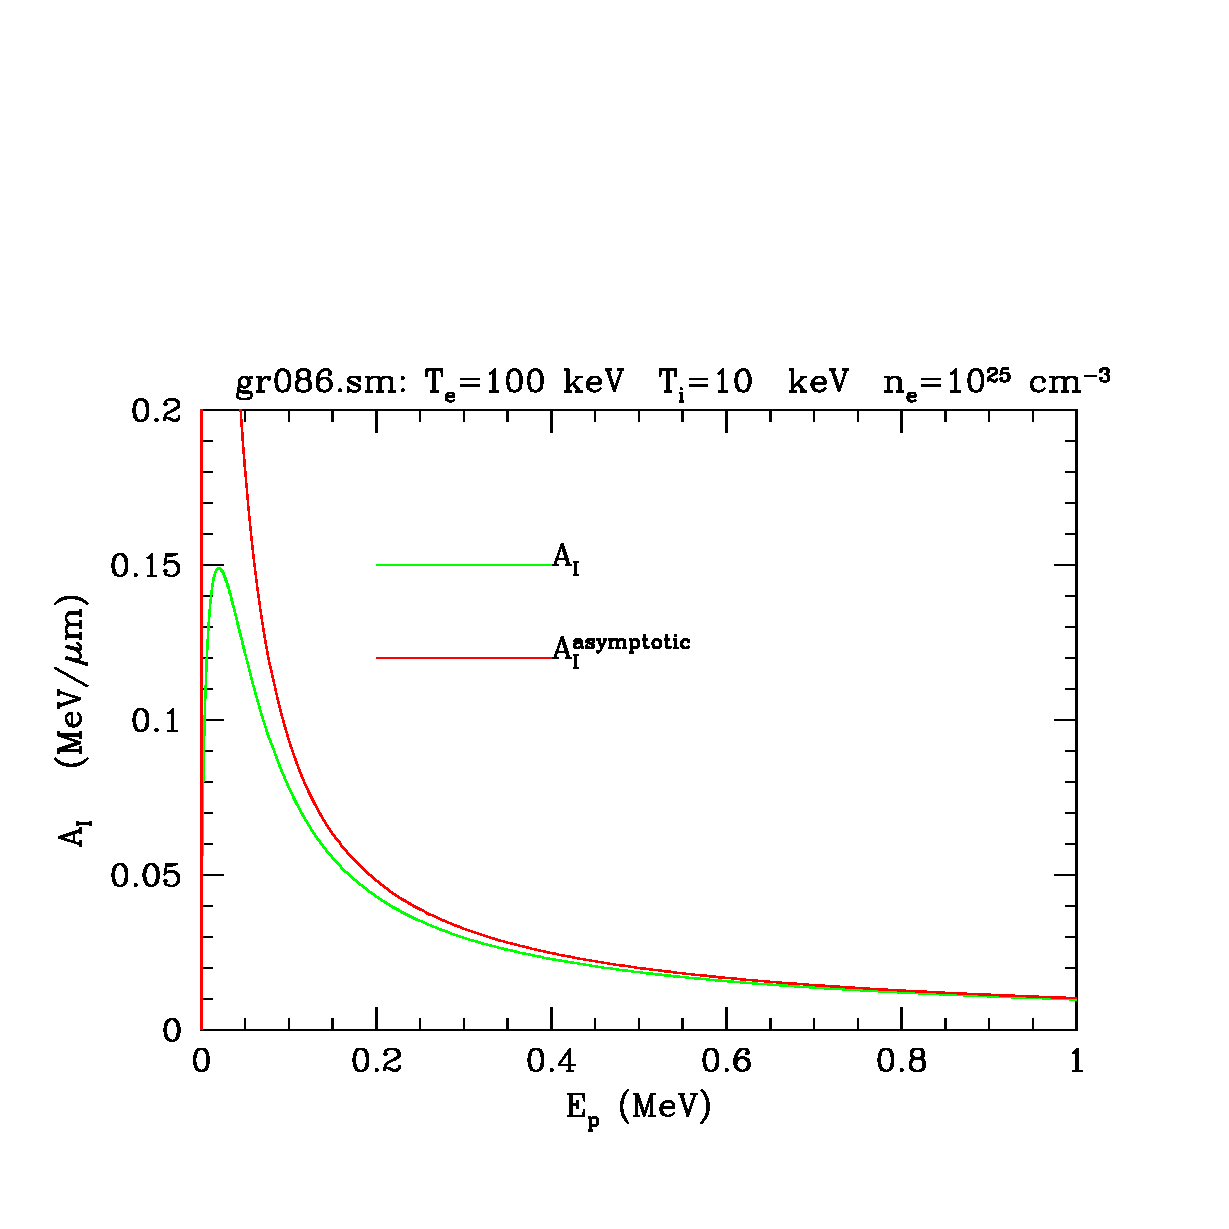
\includegraphics[scale=0.45]{gr086.eps} 
\vskip-0.8cm 
\caption{\footnoteskip  
%%
  Total asymptotic ion contribution at high energies. [gr003.f90,
  gr086.sm, gr003.dat, gr003.highE.dat, gr086.eps]
%%
}
\label{fig:gr086}
\end{figure}
%%

%%
\vskip-2cm 
\begin{figure}[h!]
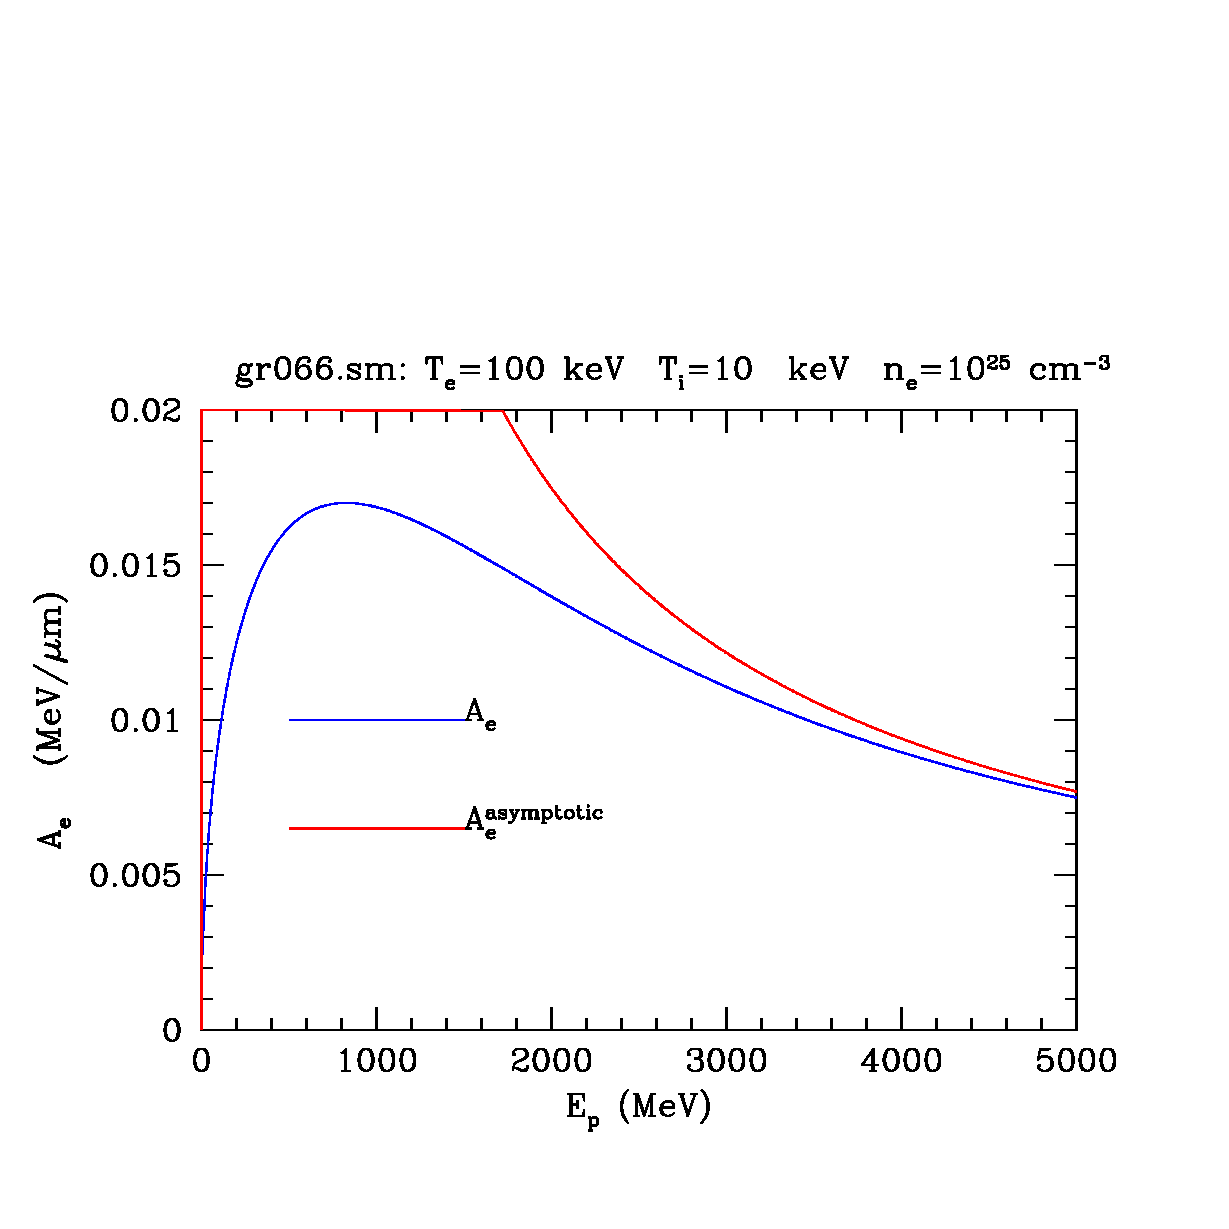
\includegraphics[scale=0.45]{gr066.eps}
\vskip-0.8cm 
\caption{\footnoteskip  
%%
  Total asymptotic electron contribution (B58) at very high
  energies. [gr003.f90, gr066.sm, gr003.dat, gr003.highEe.dat, gr066.eps]
%%
}
\label{fig:gr066}
\end{figure}
%%



\pagebreak

%%
\vskip-2cm 
\begin{figure}[h!]
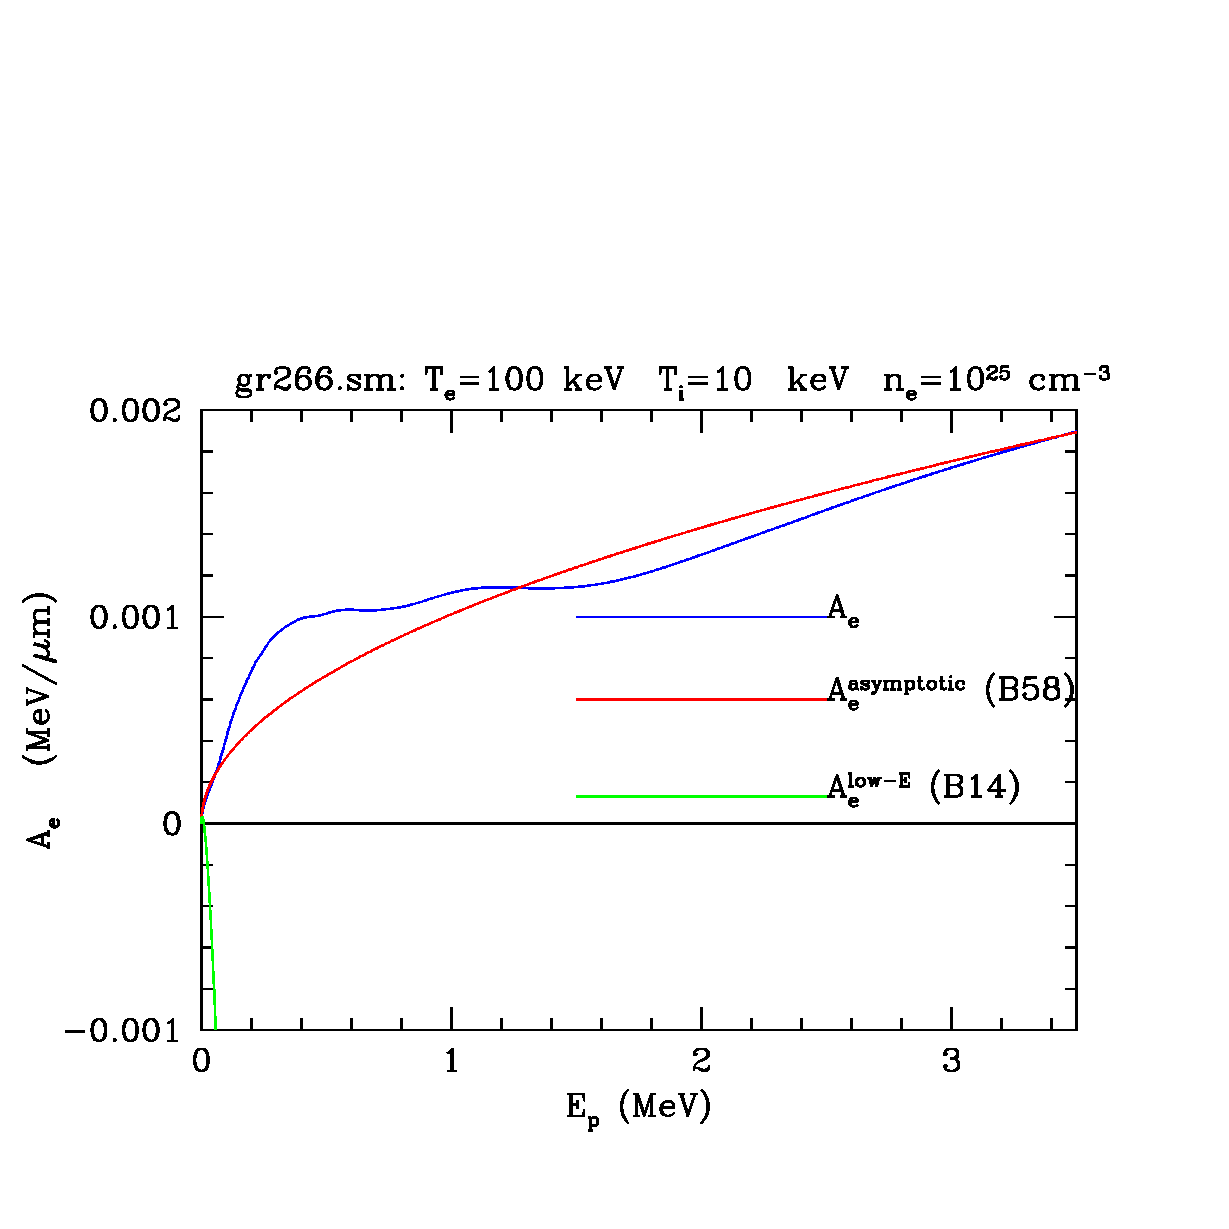
\includegraphics[scale=0.45]{gr266.eps} 
\vskip-0.8cm 
\caption{\footnoteskip  
%%
  Total asymptotic electron contribution (B56) at medium high
  energies.  [gr003.f90, gr266.sm, gr003.dat, 
  gr003.highE.dat, gr266.eps]
%%
}
\label{fig:gr266}
\end{figure}
%%

%%
\vskip-2cm 
\begin{figure}[h!]
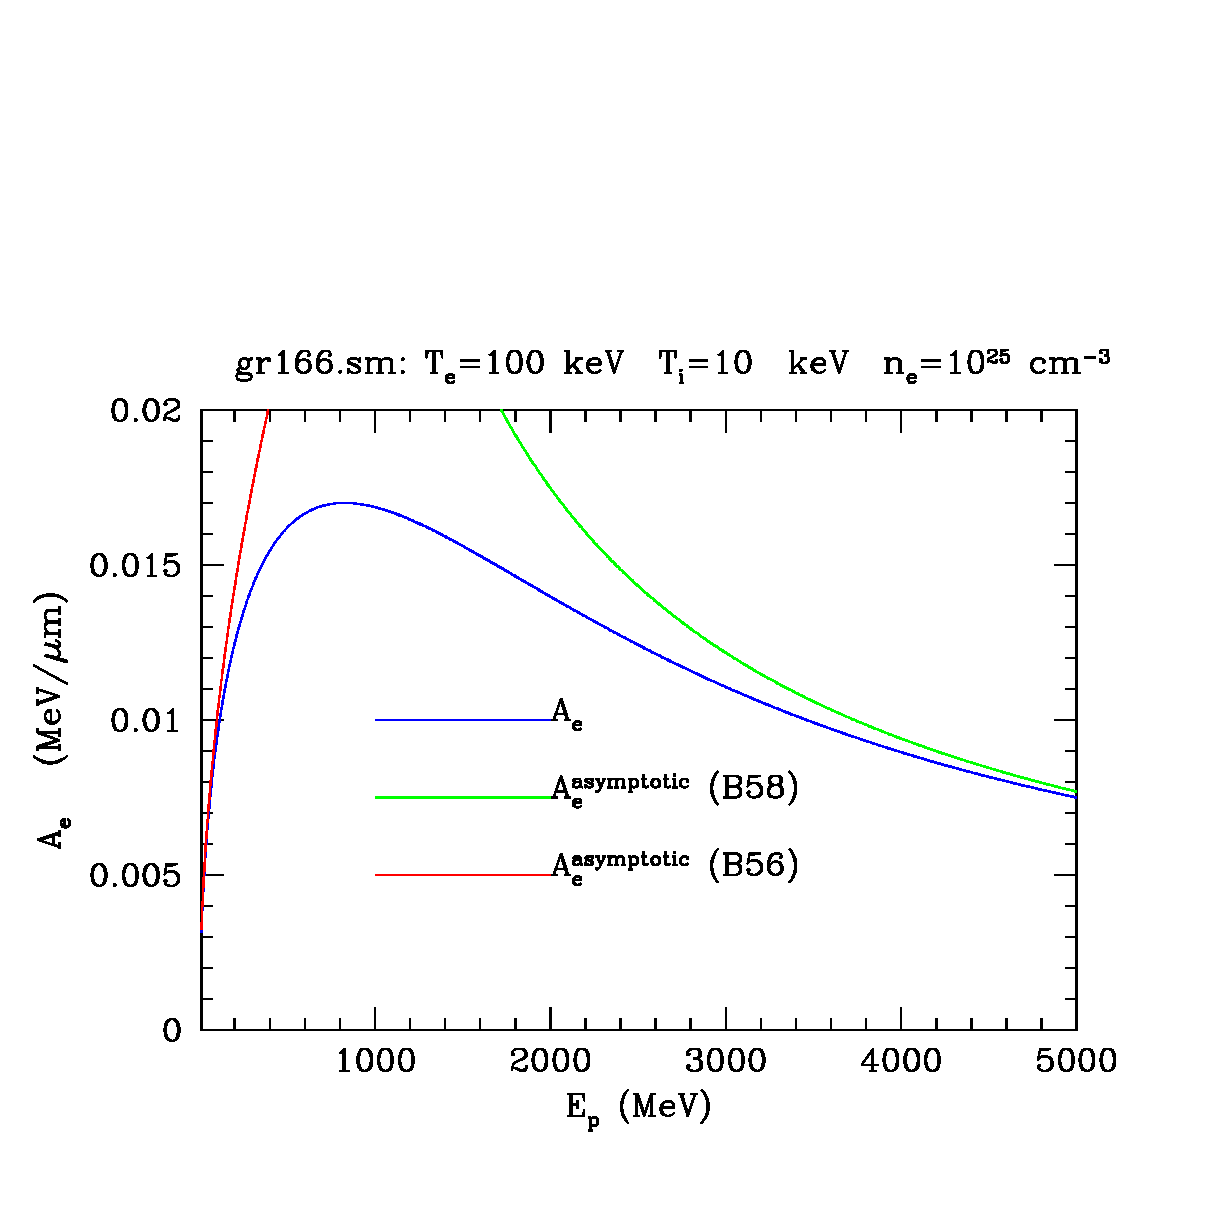
\includegraphics[scale=0.45]{gr166.eps} 
\vskip-0.8cm 
\caption{\footnoteskip  
%%
  Total asymptotic electron contribution (B56) at medium high
  energies.  [gr003.f90, gr166.sm, gr003.dat, 
  gr003.highE.dat, gr003.highEe.dat, gr166.eps]
%%
}
\label{fig:gr166}
\end{figure}
%%



\vfill
\pagebreak
\appendix
\section{Coding the A-coefficients}

\subsection{The Singular Contribution}

The singular contribution,
%%
\begin{eqnarray}
  {\cal A}^\smC_{b,\smS} 
  &=& 
  \left[
  \frac{e_p^2\, \kappa_b^2}{4\pi}
  \left( \frac{\beta_b m_b}{2\pi} \right)^{1/2} \!\! v_p
  \right]
  \int_0^1 du\, u^{1/2} e^{-\frac{1}{2}\, \beta_b m_b v_p^2 \,u}
  \left[-\ln\!\left\{\frac{\beta_b e_b e_p}{4\pi}\,K\,
  \frac{m_b}{m_{pb}}\,\frac{u}{1-u} \right\} 
  -2\gamma + 2
  \right] ,
\nonumber\\
\end{eqnarray}
%%
is quite easy to code. The integral can be broke into the pieces
%%
\begin{eqnarray}
  \int_0^1 du\, u^{1/2} e^{-\frac{1}{2}\, \beta_b m_b v_p^2 \,u}
  \Bigg[\ln\!\left\{\frac{u}{1-u} \right\} 
  -\ln\left\{\frac{\beta_b e_b e_p}{4\pi}\,K\,
  \frac{m_b}{m_{pb}}\right\} 
  -2\gamma + 2 \Bigg] \ ,
\end{eqnarray}
%%
which motivates the definition
%%
\begin{eqnarray}
  {\cal A}^\smC_{b,\smS} 
  &=& 
  c_{b, 1}\, c_{b, 2} 
  \cdot 
  {\sf A}_\smS(a_{pb},b_{pb})
\\
  {\sf A}_\smS(a,b)
  &=&
  \int_0^1 du\, u^{1/2} e^{-a \,u}
  \left[-\ln\!\left\{\frac{u}{1-u} \right\} + b \right]
\\
  a_{pb} &=& \frac{1}{2}\, \beta_b m_b v_p^2
  \hskip1cm 
  \text{and}
  \hskip1cm 
  b_{pb} =
  -\ln\left\{\frac{\beta_b e_b e_p}{4\pi}\,K\,
  \frac{m_b}{m_{pb}}\right\} -2\gamma + 2 
\\
  c_{b, 1} &=& \frac{e_p^2\, \kappa_b^2}{4\pi}
  ~~~~
  c_{b, 2} =
  \left( \frac{\beta_b m_b}{2\pi} \right)^{1/2} \! v_p  \ .
\end{eqnarray}
%%
The term involving $b$ can be integrated exactly, but we will use
Gaussian quadrature for both pieces. 

\vskip0.4cm 
\noindent
acoeff.f90:
{
\baselineskip 10pt
\begin{verbatim}
    FUNCTION dab_sing(u, a, b)
      IMPLICIT NONE  ! a=(1/2)*beta*mpc2*vp^2/C^2
      REAL,        INTENT(IN)  :: u ! [dimensionless]
      REAL,        INTENT(IN)  :: a ! [dimensionless] 
      REAL,        INTENT(IN)  :: b ! [dimensionless]
      REAL                     :: dab_sing ! [dimensionless]
      dab_sing=SQRT(u)*EXP(-a*u)*(-LOG(u/(1-u)) + b)
    END FUNCTION dab_sing
\end{verbatim}
}

\noindent
The numerical integration is performed by Gaussian quadrature:
\vskip0.4cm 
\noindent
acoeff.f90:
{
\baselineskip 10pt
\begin{verbatim}
      SUBROUTINE a_sing(a, b, ac_s)
        REAL,    INTENT(IN)  :: a
        REAL,    INTENT(IN)  :: b
        REAL,    INTENT(OUT) :: ac_s
        REAL                 :: u0, u1, du, u, um
        INTEGER, PARAMETER :: NS=1000            ! integration regions singular: must be even
        REAL,    PARAMETER :: UPM=0.7745966692E0 ! parameters for Gaussian Quad
        REAL,    PARAMETER :: W13=0.5555555556E0, W2=0.8888888889E0
           ac_s=0
           u0=0
           u1=1
           du=(u1-u0)/NS
           u=u0-du
           DO iu=1,NS,2 ! Gaussian quadrature
              u=u+2.E0*du
              ac_s=ac_s+W2*dab_sing(u,a,b)
              um=u-du*UPM
              ac_s=ac_s+W13*dab_sing(um,a,b)
              um=u+du*UPM
              ac_s=ac_s+W13*dab_sing(um,a,b)
           ENDDO
           ac_s=ac_s*du
      END SUBROUTINE a_sing
\end{verbatim}
}


%\pagebreak
\subsection{The Regular Contribution}


The long-distance regular contribution can be expressed as
%%
\begin{eqnarray}
  {\cal A}^\smLT_{b,\smR} 
  &=&
  \frac{e_p^2}{4\pi}
  \frac{i}{2\pi} \int_{-1}^1 du\,u\,
  \frac{\rho_b(v_p u)}{\rho_\text{total}(v_p u)}\,
  F(v_p u) \ln \left\{ \frac{F(v_p u)}{K^2} \right\}
\\[5pt]
  &=&
  \frac{e_p^2}{4\pi}
  \frac{i}{2\pi} \int_0^1 du\,u\,
  \frac{\rho_b(v_p u)}{\rho_\text{total}(v_p u)}\,
  \left[
  F(v_p u) \ln \left\{ \frac{F(v_p u)}{K^2} \right\}
  -
  F^*(v_p u) \ln \left\{ \frac{F^*(v_p u)}{K^2} \right\}
  \right]
\\[5pt]
  &=&
  -\frac{e_p^2}{4\pi}
  \frac{1}{2\pi} \int_0^1 du\,u\,
  \frac{\rho_b(v_p u)}{\rho_\text{total}(v_p u)}\, H(v_p u) \ ,
\end{eqnarray}
%%
where we have defined
%%
\begin{eqnarray}
  H(v) 
  &\equiv&
  -i\left[
  F(v) \ln\!\left\{ \frac{F(v)}{K^2}\right\} -
  F^*(v)\ln\!\left\{\frac{F^*(v)}{K^2} \right\}\right]
  =
  2\left[
  F_\smRe\, {\rm arg}\{F\}
  +
  F_{\smIm} \ln\!\left\{\frac{\vert F \vert}{K^2}\right\}
   \right] \ .
\nonumber\\
\label{Hbagain}
\end{eqnarray}
%%
We shall factor out a dimensionfull wavenumber $K$ and define
dimensionless quantities $\mathbb{F}(v)$ and $\mathbb{H}(v)$
through
%%
\begin{eqnarray}
  F(v) &=& K^2\,  \mathbb{F}(v) 
  ~~~\text{and}~~~
  H(v) = K^2\,  \mathbb{H}(v) \ .
\end{eqnarray}
%%
Defining the parameters
%%
\begin{eqnarray}
  a_c
  &\equiv&
  \left(\frac{\beta_c m_c}{2} \right)^{1/2}
\\[5pt]
  \bar\kappa_c^2 
  &\equiv &
  \frac{\kappa_c^2}{K^2} 
\end{eqnarray}
%%
gives the real and imaginary parts of $\mathbb{F}$, 
%%
\begin{eqnarray}
  \mathbb{F}_\smRe(\{a_c v\},\{\bar\kappa_c\}) &=& 
  {\sum}_c \bar\kappa_c^2 \Big(1 - 2 a_c\, v\,{\rm daw}\{a_c\, v\}\Big)
\label{defFreA}
\\[5pt]
  \mathbb{F}_\smIm(\{a_c v\},\{\bar\kappa_c\}) &=& 
  \sqrt{\pi}\,{\sum}_c \bar\kappa_c^2\,a_c v\, e^{-a_c^2\, v^2} \ .
\label{defFimA}
\end{eqnarray}
%%
The ratio of weighting factors can be written
%%
\begin{eqnarray}
  \frac{\kappa_b^2}{K^2}\,
  \mathbb{R}_b(\{ (u\,\beta_c m_c v_p^2/2)^{1/2}\, \}) \equiv
  \frac{\rho_b(v_p u)}{\rho_\text{total}(v_p u)}
  &=&
  \frac{
  \kappa_b^2 \left(\beta_b m_b/2\pi\right)^{1/2} \,v_p u\,
  e^{-\frac{1}{2}\,\beta_b m_b v_p^2\, u^2}}
  {{\sum}_c\kappa_c^2 \left(\beta_c m_c/2\pi\right)^{1/2} 
  \, v_p u\,  e^{-\frac{1}{2}\,\beta_c m_c v_p^2\, u^2}}
\\[5pt]
  &=&
  \left[
  {\sum}_c \, \frac{\kappa_c^2}{\kappa_b^2} 
  \left(\frac{\beta_c m_c}{\beta_b m_b}\right)^{1/2} 
  e^{\frac{1}{2}\,(\beta_b m_b-\beta_c m_c) v_p^2\, u^2}
  \right]^{-1} \ ,
\nonumber \\ 
\end{eqnarray}
%%
or
%%
\begin{eqnarray}
  \mathbb{R}_b(\{ (u\,\beta_c m_c v_p^2/2)^{1/2}\, \}) 
  =
  \left[
  {\sum}_c \, \frac{\kappa_c^2}{K^2} 
  \left(\frac{\beta_c m_c}{\beta_b m_b}\right)^{1/2} 
  e^{\frac{1}{2}\,(\beta_b m_b-\beta_c m_c) v_p^2\, u^2}
  \right]^{-1} \ .
\end{eqnarray}
%%
We can now express the regular piece as
%%
\begin{eqnarray}
  {\cal A}^\smC_{b,\smR}
  &=& 
  \underbrace{
  \left[
  \frac{e_p^2\, \kappa_b^2}{4\pi}\,
  \right] 
  }_{c_{b,1}}
  \cdot \,
  {\sf A}_\smR(v_p,\{a_c\},\{\bar\kappa_c\})
\\
  {\sf A}_{b\,\smR}(v_p,\{a_c\},\{\bar\kappa_c\})
  &=&
  \int_0^1 du\, 
  \underbrace{
  \mathbb{R}_b(\{a_c v_p u\})\,
  \mathbb{H}(\{a_c\,v_p u\},\{\bar\kappa_c\})  
  }_{\rm dab\_reg}
  \ .
\end{eqnarray}
%%

\vskip0.4cm
\noindent
acoeff.f90:
{
\baselineskip 10pt
\begin{verbatim}
      FUNCTION dab_reg(u, vp, ib, nni, k2, kb2, betab, mb)
      USE mathvars
      USE physvars
        IMPLICIT NONE
        REAL,                        INTENT(IN)  :: u       !  [dimensionless]
        REAL,                        INTENT(IN)  :: vp      !  Projectile velocity [cm/s]
        INTEGER,                     INTENT(IN)  :: ib      !  Species number
        INTEGER,                     INTENT(IN)  :: nni     !  Number of ion species
        REAL,                        INTENT(IN)  :: k2      !  Wavenumber squared [1/cm^2]
        REAL,    DIMENSION(1:nni+1), INTENT(IN)  :: kb2     !  Debye wavenumber squared [1/cm^2]
        REAL,    DIMENSION(1:nni+1), INTENT(IN)  :: betab   !  Temperature array [1/keV]
        REAL,    DIMENSION(1:nni+1), INTENT(IN)  :: mb      !  Mass array [keV]
        REAL                                     :: dab_reg !  [dimensionless]
        REAL,    DIMENSION(1:nni+1) :: alfb, ab
        REAL                        :: fr, fi, fabs, farg, h
        REAL                        :: kcb, r_ib, bm_ic, bm_ib, a_ic, a_ib, ex, au
        INTEGER                     :: ic
        ab=SQRT(0.5*betab*mb)*vp/CC
        alfb=kb2/k2
        CALL frfi(u,nni,alfb,ab,fr,fi,fabs,farg)
        h=2*(fr*farg + fi*LOG(fabs))
!
! construct spectral weight ratio Rb=rho_b/rho_tot
!
        r_ib=0
        bm_ib=betab(ib)*mb(ib)
        a_ib =ab(ib)*ab(ib)
        DO ic=1,nni+1
           kcb=kb2(ic)/k2
           bm_ic=betab(ic)*mb(ic)
           a_ic =ab(ic)*ab(ic)
           IF (ic == ib) THEN
              ex=1
           ELSE
              au=(a_ic-a_ib)*u
              ex=EXP(-au)
           ENDIF
           r_ib=r_ib + kcb*SQRT(bm_ic/bm_ib)*ex
        ENDDO      
        r_ib=1/r_ib
        dab_reg=-u*r_ib*h/TWOPI
      END FUNCTION dab_reg
\end{verbatim}
}

\noindent
The numerical integration is performed by Gaussian quadrature:
\vskip0.4cm
\noindent
acoeff.f90:
{
\baselineskip 10pt
\begin{verbatim}
      SUBROUTINE a_reg(ib, nni, vp, k2, kb2, betab, mb, ac_r)
        INTEGER,                     INTENT(IN)  :: ib
        INTEGER,                     INTENT(IN)  :: nni 
        REAL,                        INTENT(IN)  :: k2
        REAL,                        INTENT(IN)  :: kb2
        REAL,    DIMENSION(1:nni+1), INTENT(IN)  :: betab
        REAL,    DIMENSION(1:nni+1), INTENT(IN)  :: mb
        REAL,                        INTENT(OUT) :: ac_r
        REAL               :: u0, u1, du, u, um
        INTEGER, PARAMETER :: NR=10            ! integration regions singular: must be even
        REAL,    PARAMETER :: UPM=0.7745966692E0 ! parameters for Gaussian Quad
        REAL,    PARAMETER :: W13=0.5555555556E0, W2=0.8888888889E0
        ac_r=0
        u0=0.
        u1=1.
        du=(u1-u0)/NR
        u=u0-du
        DO iu=1,NR,2 ! Gaussian quadrature
           u=u+2.E0*du
           ac_r=ac_r+W2*dab_reg(u,vp,ib,nni,k2,kb2,betab,mb)
           um=u-du*UPM
           ac_r=ac_r+W13*dab_reg(um,vp,ib,nni,k2,kb2,betab,mb)
           um=u+du*UPM
           ac_r=ac_r+W13*dab_reg(um,vp,ib,nni,k2,kb2,betab,mb)
        ENDDO
        ac_r=ac_r*du
      END SUBROUTINE a_reg
\end{verbatim}
}


%\pagebreak
\subsection{Quantum Contribution}

For the quantum term we make the change of variables
$v_{pb}= v_p\,u$ so that
%%
\begin{eqnarray}
  {\cal A}^\smQM_b
  &\!=\!&  
  -\frac{e_p^2\, \kappa_b^2}{4\pi}\,
  \left( \frac{\beta_b m_b}{2\pi} \right)^{1/2} \!\! v_p\,
  \int_0^\infty du\, 
  \Big[{\rm Re}\,\psi\!\left\{ 1 + i\, \frac{\bar\eta_{pb}}{u}
  \right\}
  - \ln\!\left\{\frac{\bar\eta_{pb}}{u} \right\} \Big] 
  \frac{1}{\beta_b m_b v_p^2\,u}
\nonumber
\\ &&
  \Bigg[ e^{-\frac{1}{2}\,\beta_b m_b v_p^2 (u-1)^2} 
  \left(1 - \frac{1}{\beta_b m_b v_p^2\, u}\right) +
  e^{-\frac{1}{2}\,\beta_b m_b v_p^2 (u+1)^2}  
  \left(1 + \frac{1}{\beta_b m_b v_p^2\, u}\right)
  \Bigg] \ .
\end{eqnarray}
%%
The quantum function we need to code is therefore
%%
\begin{eqnarray}
  {\cal A}^\smQM_b
  &\!=\!&  
  \underbrace{
  \left[\frac{e_p^2\, \kappa_b^2}{4\pi}\,
  \left( \frac{\beta_b m_b}{2\pi} \right)^{1/2} \!\! v_p\,
  \right] 
  }_{c_{b, 1} \cdot c_{b, 2}}
  \cdot \,
  {\sf A}_1^\smQM(a_{pb}, \tilde\eta_{pb}) \ ,
\label{qmA}
\end{eqnarray}
%%
where the arguments of the function are defined by 
%%
\begin{eqnarray}
  a_{pb} 
  &=& 
  \frac{1}{2}\,\beta_b m_b\, v_p^2
\\
  \tilde\eta_{pb}
  &=& 
  \frac{e_p e_b}{4 \pi \hbar v_p}
  =
  \vert Z_p Z_b\vert\,\frac{e^2}{8 \pi a_0}\,\frac{2 a_0}{\hbar}\,
  \frac{1}{v_p}
  =
  \vert Z_p Z_b\vert\ \cdot 13.606\,{\rm eV}\,\cdot
  \frac{2 \cdot 5.29 \times 10^{-9}\,{\rm cm}}{6.5821 \times
  10^{-16}\,{\rm eV\,s}}\,
  \frac{1}{v_p}
\nonumber
\\
  &=&
  2.1870 \times 10^8 \, \frac{\vert Z_p Z_b\vert}{v_p
  \cdot ({\rm cm/s})^{-1}} \ ,
\end{eqnarray}
%%
and the function itself takes the form
%%
\begin{eqnarray}
  {\sf A}_1^\smQM(a,\eta)
  &\!=\!&  
  -\int_0^\infty \! du\, 
  \left[{\rm Re}\,\psi\! \left\{1 + i\, \frac{\eta}{u} \right\} - 
  \ln\left\{ \frac{\eta}{u}  \right\} \right]
\nonumber
\\ && 
  \frac{1}{2 a\,u}\left[\left(e^{-a(u-1)^2} + e^{-a(u+1)^2} \right) 
  - \frac{e^{-a(u-1)^2} - e^{-a(u+1)^2} } {2 a\, u}\right] \ .
\label{qmAB}
\end{eqnarray}


\vskip1cm 
\noindent
acoeff.f90:
{
\baselineskip 10pt
\begin{verbatim}
      FUNCTION daq(u, a, eta)
      USE physvars
        IMPLICIT NONE
        REAL,                        INTENT(IN)  :: u          ! [dimensionless]
        REAL,                        INTENT(IN)  :: a          ! [dimensionless]
        REAL,                        INTENT(IN)  :: eta        ! [dimensionless]
        REAL                                     :: daq  ! [dimensionless]
        REAL, PARAMETER :: AMAX=25.
        REAL            :: repsi, au, eu, au2, ap, am, psilog, ch, sh
        eu=eta/u 
        psilog=repsi(eu) - LOG(eu)
        au =2*a*u
        au2=a*u*u
        IF (a <= AMAX) THEN      
          ch =EXP(-au2)*COSH(au)
          sh =EXP(-au2)*SINH(au)
        ELSE
          ap = au-au2-a
          am =-au-au2-a
          ch =0.5*(EXP(ap)+EXP(am))
          sh =0.5*(EXP(ap)-EXP(am))
        ENDIF
        daq=-psilog*2*(ch - sh/au)/au
      END FUNCTION daq


      SUBROUTINE a_quantum(ib, a, eta, aq)
        IMPLICIT NONE
        INTEGER, INTENT(IN)  :: ib    ! species index
        REAL,    INTENT(IN)  :: a     ! [dimensionless] (1/2) betab mb vp^2
        REAL,    INTENT(IN)  :: eta   ! [dimensionless] ep eb/4pi hbar vp
        REAL,    INTENT(OUT) :: aq 
        REAL               :: u0, u1, du, u, um
        INTEGER, PARAMETER :: NQ=1000            ! integration regions quantum : must be even
        REAL,    PARAMETER :: UPM=0.7745966692E0 ! parameters for Gaussian Quad
        REAL,    PARAMETER :: W13=0.5555555556E0, W2=0.8888888889E0
        REAL    :: daq
        INTEGER :: iu
        aq=0
        u0=0.
        aq=0
        IF (ib == 1) THEN
           u0=0
           u1=4./SQRT(a)
        ELSE
           u0=1-10./SQRT(a)
           u0=MAX(0.,u0)  
           u1=1+10./SQRT(a)
        ENDIF
        du=(u1-u0)/NQ
        u=u0-du
        DO iu=1,NQ,2 ! Gaussian quadrature
           u=u+2.E0*du
           aq=aq+W2*daq(u,a,eta)
           um=u-du*UPM
           aq=aq+W13*daq(um,a,eta)
           um=u+du*UPM
           aq=aq+W13*daq(um,a,eta)
        ENDDO
        aq=aq*du
      END SUBROUTINE a_quantum
\end{verbatim}
}


\pagebreak
\section{Complete Source Code Listing: \lowercase{acoeff.f90} }

This section gives the complete listing for the source acoeff.f90 as
it currently stands, including comments for the user and comments that
I have made for myself (the latter will eventually disappear). This
source module calculates the {\cal A}-coefficients (coeff\_bps), their
low energy asymptotic limits (coeff\_bps\_small\_E), and their high
energy asymptotic limits (coeff\_bps\_high\_E). For the electron,
there are two distinct high energy regions: an intermediate high
energy regime $T \ll E_p \ll (m_\smI/m_e)\,T$ and an extreme high
energy regime $E \gg (m_\smI/m_e)\,T$.


\vskip0.5cm
\noindent
Note: Currently, the subroutine coeff\_bps\_high\_E only returns the
total electron contribution ${\cal A}_e$ (regular + singular + quantum).



\vskip0.5cm
\noindent
To do: To complete the subroutine coeff\_bps\_high\_E, I need to
calculate the regular and singular contributions for the electrons in
both high energy regimes. That is to say, I need to calculate the
asymptotic limits of ${\cal A}_{e \,,\,\smS}^\smC$ and ${\cal A}_{e
\,,\,\smR}^\smLT$ respectively. The quantum asymptotic correction
can then be obtained by
  $$
  {\cal A}_e^\smQM = {\cal A}_e - {\cal A}_e^\smC = 
  {\cal A}_e - ({\cal A}_{e\,,\,\smS}^\smC + {\cal A}_{e
  \,,\,\smR}^\smLT ).
  $$ 
Before coeff\_bps\_high\_E returns the same quantities for electrons
and ions, I will need to analytically calculate ${\cal A}_{e \, ,
\,\smS}^\smC$ and ${\cal A}_{e \,, \, \smR}^\smLT$ and their high
energy limits. To repeat the above note: until I finish this
calculation, the subroutine coeff\_bps\_high\_E only returns the total
electron contribution ${\cal A}_e$, although it returns the complete
set of contributions for ${\cal A}_\smI$. 

\subsection{The {\cal A}-Coefficients}

\vskip1cm 
\noindent
acoeff.f90:
{
\baselineskip 10pt
\begin{verbatim}

! 
! ROUTINE: bps_acoeff_ab_mass(nni, ep, mp, zp, ia, ib, betab, zb, mb, nb, &
!            a_ab, a_ab_sing, a_ab_reg, a_ab_qm)
! 
! Assume a plasma composed of several species b, each separately in 
! thermal equilibrium with themselves but not necessarily with each 
! other[1]. This routine returns several useful components of the 
! corresponding A-coefficients introduced in Note [2] below (BPS).
! 
! UNITS: A_{pb} has units of [MeV/micron] (subject to change in updates)
! 
! THE PHYSICS:
! The various subsystems b will exchange coulomb energy and they will
! eventually equilibrate to a common temperature. The A-coefficients 
! introduced in Ref. [2] encode this coulomb energy exchange, exactly to 
! leading and next-to-leading orders in the plasma coupling constant g.
! See Refs. [3,4,5] for more details. For a weakly coupled plasma (g << 1), 
! the BPS calculation is essentially exact, and the error is O(g). Physical 
! properties of interest, such as the stopping power dE/dx and the temperature 
! equilibration rate between plasma species, can be obtained directly from 
! the A-coefficients. 
!
! USAGE:
! Since electrons are thousands of times lighter than ions, one of the most
! physically accessible regime is the in which the electrons have a temperature 
! T_e and the ions have a (possibly different) common temperature T_I. This 
! is why the output is organized into electron contributions and total ion 
! contributions (sum over all ions).
!
! INPUT: nni, ep, zp, mp, ia, ib, betab, zb, mb, nb
!
! Describe the incident projectile and the background plasma. 
!
! projectile input quantities:
! ep : classical kinetic energy of the projectile [keV]
! zp : charge of the projectile in units of Z_p [dimensionless]
! mp : mass of the projectile [keV], i.e. mp = mp[grams]*c^2
!
! plasma input quantities:
! nni  : Number of total plasma species = number ion species + 1
! zb   : Charges of the plasma species. By convention zp(1) is the 
!      : electron plasma component. [dimensionless, Array]
! betab: Inverse temperatures of the plasma components. For an
!        electron-ion plasma, set betab(1)=1/T_e and all other
!        values of the array to 1/T_I [keV^-1].
! mb   : Masses of the plasma species [keV]. 
! nb   : Number densities of the plasma species [cm^-3]. 
! ia   : First plasma species [usually the projectile]
! ib   : Second plasma species
!
! OUTPUT: a_ab, a_ab_sing, a_ab_reg, a_ab_qm
!
! Each plasma component b makes a linear contribution A_b to the total 
! A-coefficient, i.e. A = sum_b A_b [5]. Each A_b in turn can be be 
! decomposed into a classical-quantum or electron-ion contributions.
!
! classical electron  : ac_e
! classical ion       : ac_i [sum over all ions]
! classical total     : ac_tot = ac_e + ac_i 
! quantum   electron  : aq_e
! quantum   ion       : aq_i [sum over all ions]
! quantum   total     : a_tot = aq_e + aq_i
! total     electric  : a_e = ac_e + aq_e
! total     ion       : a_i = ac_i + aq_i
! total               ! a_tot = a_e + a_i
!
! NOTES:
! [1] The temperatures T_b may therefore all differ. By convention
!     I take b=1 for the electron component of the plasma. A very
!     useful and interesting parameter regime is the one in which 
!     the ions have a common temperature T_I and the electron have
!     a temperature T_e, usually with T_e =/= T_I.  See also USAGE
!     and note [3] below.
!
! [2] BPS paper
!     L. Brown, D. Preston, and R. Singleton~Jr., 
!     "Charged Particle Motion in a Highly Ionized Plasma",
!     Physics Reports, 410 (2005) 237
!     [arXiv:physics/0501084]
!
! [3] The code employs rationalized cgs units in which the dimensionless
!     plasma coupling parameter is defined by g = e^2 kappa/(4Pi*T); in 
!     these units the Debye wavenumber is determined by kappa^2 = e^2 n/T 
!     and the plasma frequency by omega^2 = e^2 n/m. A weakly coupled 
!     plasma is one for which g << 1, i.e. a plasma with thermal kinetic 
!     energy (of order the temperature T) dominates the coulomb potential 
!     energy (for particles separated by a Debye length). In the more 
!     common non-rationalized cgs units, we define g = e^2 kappa/T, with 
!     kappa^2 = 4 Pi e^2 n/T and omega^2 = 4 Pi e^2 n/m. 
!
! [4] For coulomb energy exchange processes, the leading and next-to-
!     leading order terms in the plasma coupling g are proportional to 
!     g^2*ln(g) and g^2, respectively. That is to say, for a property 
!     denoted by F, one can expand F in powers of g in the form:
!
!       F(g,eta) = A(eta)*g^2*ln(g) + B(eta)*g^2 + O(g^3) 
!                 = A(eta)*g^2*[ ln(C(eta)*g)+O(g) ],
!
!     where eta is the dimensionless quantum parameter (eta <<1 means
!     extreme classical scattering while eta >>1 means the extreme quantum 
!     limit). The relative error of BPS is therefore O(g). At the center of 
!     the sun g=0.4, and so the error of Ref. [1] is only of order 4% in 
!     this case. For the processes of charged stopping power and electron-
!     ion temperature equilibration, Ref. [1] calculates the corresponding
!     functions A(eta) and B(eta) exactly, including all orders in the 
!     two-body quantum scattering parameter eta = e^2/4Pi*hbar*v_thermal 
!     (this means that BPS gives the correct interpolation between the 
!     classical and quantum regimes, exact to leading and next-to-leading 
!     order). The O(g^3) terms physically correspond to 3-body correlations 
!     within the plasma, and for a sufficiently weak plasma these are 
!     negligible. For strongly coupled plasmas (g >> 1), all terms in a 
!     g-expansion are important and the BPS calculation is not applicable.
!
! [5] It makes sense to talk about separate linear contribution A_b
!     contributing *from* a given plasma component b only for a weakly 
!     coupled plasma. More exactly, A=sum_b A_b holds true only up to 
!     leading and next-to-leading order in the plasma coupling g. This is 
!     the order to which Ref. [2] calculates all quantities, and therefore 
!     BPS works to a consistent order in g.
!
!
! vp = projectile speed [cm/s]
!
!            [ 2 Ep ]
!    = c sqrt[ ---- ]  where mp and Ep are in keV and
!            [ mpc2 ]  c is the speed of light in cm/s
!
!
!        ep^2 kb^2
! c1  =  --------- = 2 zp**2 * Be * kb^2 * a0  [keV/cm]
!           4 Pi                               [MeV/micron]
!
!       [ betab mbc2 ]^1/2  
! c2 =  |----------- |      vp   [dimensionless]
!       [   2 Pi     ]      
!        
! where
!          e^2 
! Be  =  --------- = 13.606E-3   [keV]
!        8 Pi a0                 Bohr radius: a0=5.29E-9 cm
!
!
!
!
!%%%%%%%%%%%%%%%%%%%%%%%%%%%%%%%%%%%%%%%%%%%%%%%%%%%%%%%%%%%%%%%%%%%%%%%%%%%%
! main driver for A-coefficient for general quantum and electron-mass regimes
!%%%%%%%%%%%%%%%%%%%%%%%%%%%%%%%%%%%%%%%%%%%%%%%%%%%%%%%%%%%%%%%%%%%%%%%%%%%%
!
      SUBROUTINE bps_acoeff_ab_mass(nni, ep, mp, zp, ia, ib, betab, zb, mb, nb, &
            a_ab, a_ab_sing, a_ab_reg, a_ab_qm)
      USE physvars
      USE mathvars    
        IMPLICIT NONE                                             ! Plasma:
        INTEGER,                            INTENT(IN)  :: nni    !  number of ions
        REAL,                               INTENT(IN)  :: ep     !  energy input [keV]
        REAL,                               INTENT(IN)  :: mp     !  mass [keV]
        REAL,                               INTENT(IN)  :: zp     !  charge
        INTEGER,                            INTENT(IN)  :: ia     !  
        INTEGER,                            INTENT(IN)  :: ib     !  
        REAL,    DIMENSION(1:nni+1),        INTENT(IN)  :: betab  !  temp array [1/keV]
        REAL,    DIMENSION(1:nni+1),        INTENT(IN)  :: mb     !  mass array [keV]
        REAL,    DIMENSION(1:nni+1),        INTENT(IN)  :: nb     !  density [1/cc]
        REAL,    DIMENSION(1:nni+1),        INTENT(IN)  :: zb     !  charge array
                                                                  !
                                                                  ! A-coeffs [MeV/micron]
        REAL,                               INTENT(OUT) :: a_ab
        REAL,                               INTENT(OUT) :: a_ab_sing
        REAL,                               INTENT(OUT) :: a_ab_reg
        REAL,                               INTENT(OUT) :: a_ab_qm

        REAL,    DIMENSION(1:nni+1)  :: mpb, mbpb, kb2, ab
        REAL                         :: vp, zp2, k, k2, kd, kd2, a, b, eta
        REAL                         :: ac_r, ac_s, aq, c1, c2

        REAL, PARAMETER              :: EPS_SMALL_E=2.E-4
        REAL, PARAMETER              :: EPS_SMALL_E_SING=2.E-4
        REAL, PARAMETER              :: EPS_SMALL_E_REG=2.E-4
!
! initialize components of A-coefficients
!
        kb2=8*PI*A0CM*BEKEV*zb*zb*nb*betab
        kd2 = SUM(kb2)                ! [1/cm^2]
        kd  = SQRT(kd2)               ! [1/cm]
        k2  = kb2(1)                  ! [1/cm^2]
        k   = SQRT(k2)                ! [1/cm]   k = k_e
!
! Loop over charged plasma species
!
        mpb = mp*mb/(mp+mb)            ! [keV]
        mbpb= mb/mpb                   ! [dimensionless]
        vp =CC*SQRT(2*ep/mp)           ! [cm/s]
        zp2=zp**2                      ! [dimensionless]
                                       ! ab=(1/2) betab(ib)*mbc2(ib)*vp2/CC2
        ab  =0.5*betab*mb*vp*vp/CC2    ! [dimensionless] 
        IF (zb(ib) .NE. 0.) THEN
        a  =ab(ib)
        b  =-Log(2*betab(ib)*BEKEV*ABS(zp*zb(ib))*k*A0CM*mbpb(ib) )-2*GAMMA+2
        eta=ABS(zp*zb(ib))*2.1870E8/vp ! defined with projectile velocity vp
        c1=2*zp2*BEKEV*kb2(ib)*A0CM    ! [keV/cm] c1 = e_p^2 kappa_b^2/(4 Pi)
        c1=c1*1.E-7                    ! [MeV/micron]  
        c2=SQRT(a/PI)                  ! [dimensionless] 
                                       ! c2=SQRT(betab(ib)*mb(ib)/TWOPI)*vp/CC 
!
! A_{ab}-classical-singular 
!
        CALL a_sing_mass(a,b,ac_s) 
        a_ab_sing=c1*c2*ac_s
!
! A_{ab}-classical-regular 
!
        CALL a_reg_mass(nni,ia,ib,vp,k2,kb2,betab,mb,ac_r)
        a_ab_reg=c1*ac_r
!
! A_{ab}-quantum
!
        CALL a_quantum_mass(ia,ib,a,eta,aq) ! eta = dimensionless quantum param.
        a_ab_qm=c1*c2*aq
!
! A_{ab}-total
!
        a_ab=a_ab_sing + a_ab_reg + a_ab_qm
        ENDIF
      END SUBROUTINE bps_acoeff_ab_mass
!
!%%%%%%%%%%%%%%%%%%%%%%%%%%%%%%%%%%%%%%%%%%%%%%%%%%%%%%%%%%%%%%%%%%%%%%%%%%%%
! Assembles the matrix A_{ab} of the A-coefficients.
!%%%%%%%%%%%%%%%%%%%%%%%%%%%%%%%%%%%%%%%%%%%%%%%%%%%%%%%%%%%%%%%%%%%%%%%%%%%%
!
      SUBROUTINE bps_acoeff_ab_matrix(nni, ep, betab, zb, mb, nb,    &
        a_ab, a_ab_sing, a_ab_reg, a_ab_qm, a_tot, a_i, a_e, ac_tot, &
        ac_i, ac_e, aq_tot, aq_i, aq_e, ac_s_i, ac_s_e, ac_r_i, ac_r_e)
      USE physvars
      USE mathvars    
        IMPLICIT NONE                                             ! Plasma:
        INTEGER,                            INTENT(IN)  :: nni    !  number of ions
        REAL,                               INTENT(IN)  :: ep     !  energy
        REAL,    DIMENSION(1:nni+1),        INTENT(IN)  :: betab  !  temp array [1/keV]
        REAL,    DIMENSION(1:nni+1),        INTENT(IN)  :: zb     !  charge array
        REAL,    DIMENSION(1:nni+1),        INTENT(IN)  :: mb     !  mass array [keV]
        REAL,    DIMENSION(1:nni+1),        INTENT(IN)  :: nb     !  density [1/cc]
                                                                  !
                                                                  ! A-coeffs [MeV/micron]
        REAL,    DIMENSION(1:nni+1,1:nni+1),INTENT(OUT) :: a_ab
        REAL,    DIMENSION(1:nni+1,1:nni+1),INTENT(OUT) :: a_ab_sing
        REAL,    DIMENSION(1:nni+1,1:nni+1),INTENT(OUT) :: a_ab_reg
        REAL,    DIMENSION(1:nni+1,1:nni+1),INTENT(OUT) :: a_ab_qm
        REAL,    DIMENSION(1:nni+1),        INTENT(OUT) :: a_tot
        REAL,    DIMENSION(1:nni+1),        INTENT(OUT) :: a_i
        REAL,    DIMENSION(1:nni+1),        INTENT(OUT) :: a_e
        REAL,    DIMENSION(1:nni+1),        INTENT(OUT) :: ac_tot
        REAL,    DIMENSION(1:nni+1),        INTENT(OUT) :: ac_i
        REAL,    DIMENSION(1:nni+1),        INTENT(OUT) :: ac_e
        REAL,    DIMENSION(1:nni+1),        INTENT(OUT) :: aq_tot
        REAL,    DIMENSION(1:nni+1),        INTENT(OUT) :: aq_i
        REAL,    DIMENSION(1:nni+1),        INTENT(OUT) :: aq_e
        REAL,    DIMENSION(1:nni+1),        INTENT(OUT) :: ac_s_i
        REAL,    DIMENSION(1:nni+1),        INTENT(OUT) :: ac_s_e
        REAL,    DIMENSION(1:nni+1),        INTENT(OUT) :: ac_r_i
        REAL,    DIMENSION(1:nni+1),        INTENT(OUT) :: ac_r_e

        REAL    :: aab, aab_sing, aab_reg, aab_qm
        REAL    :: mp, zp
        INTEGER :: ia, ib

        a_i   = 0
        ac_s_i= 0
        ac_r_i= 0
        ac_i  = 0
        aq_i  = 0
        DO ia=1,nni+1
          mp=mb(ia)
          zp=zb(ia)
          DO ib=1,nni+1
            CALL bps_acoeff_ab_mass(nni, ep, mp, zp, ia, ib, betab, zb, mb, nb, &
            aab, aab_sing, aab_reg, aab_qm)
            a_ab(ia,ib)     =aab
            a_ab_sing(ia,ib)=aab_sing
            a_ab_reg(ia,ib) =aab_reg
            a_ab_qm(ia,ib)  =aab_qm 
            IF (ib == 1) THEN
               a_e(ia)   = aab 
               ac_s_e(ia)= aab_sing
               ac_r_e(ia)= aab_reg
               ac_e(ia)  = aab_sing + aab_reg
               aq_e(ia)  = aab_qm
            ELSE
               a_i(ia)   = a_i(ia)    + aab 
               ac_s_i(ia)= ac_s_i(ia) + aab_sing
               ac_r_i(ia)= ac_r_i(ia) + aab_reg
               ac_i(ia)  = ac_i(ia)   + aab_sing + aab_reg
               aq_i(ia)  = aq_i(ia)   + aab_qm
            ENDIF
          ENDDO
          a_tot(ia) = a_e(ia)  + a_i(ia)
          ac_tot(ia)= ac_e(ia) + ac_i(ia)
          aq_tot(ia)= aq_e(ia) + aq_i(ia)
        ENDDO
      END SUBROUTINE bps_acoeff_ab_matrix
!
!%%%%%%%%%%%%%%%%%%%%%%%%%%%%%%%%%%%%%%%%%%%%%%%%%%%%%%%%%%%%%%%%%%%%%%%%%%%%
! Returns A_{p I} = \sum_i A_{p i} for backward compatibility
!%%%%%%%%%%%%%%%%%%%%%%%%%%%%%%%%%%%%%%%%%%%%%%%%%%%%%%%%%%%%%%%%%%%%%%%%%%%%
!
      SUBROUTINE bps_acoeff_ei_mass(nni, ep, zp, mp, betab, zb, mb, nb, &
            a_tot, a_i, a_e, ac_tot, ac_i, ac_e, aq_tot, aq_i, aq_e,&
            ac_s_i, ac_s_e, ac_r_i, ac_r_e)
      USE physvars
      USE mathvars    
      USE controlvars  
        IMPLICIT NONE                                      ! Plasma:
        INTEGER,                     INTENT(IN)  :: nni    !  number of ions
        REAL,    DIMENSION(1:nni+1), INTENT(IN)  :: betab  !  temp array [1/keV]
        REAL,    DIMENSION(1:nni+1), INTENT(IN)  :: mb     !  mass array [keV]
        REAL,    DIMENSION(1:nni+1), INTENT(IN)  :: nb     !  density [1/cc]
        REAL,    DIMENSION(1:nni+1), INTENT(IN)  :: zb     !  charge array
                                                           !
                                                           ! Projectile  
        REAL,                        INTENT(IN)  :: ep     !  projectile energy [keV]
        REAL,                        INTENT(IN)  :: mp     !  projectile mass   [keV]
        REAL,                        INTENT(IN)  :: zp     !  projectile charge
                                                           !
                                                           ! A-coeffs [MeV/micron]
        REAL,                        INTENT(OUT) :: a_tot  !  electron + ion
        REAL,                        INTENT(OUT) :: a_i    !  ion contribution
        REAL,                        INTENT(OUT) :: a_e    !  electron contribution
        REAL,                        INTENT(OUT) :: ac_tot !  classical
        REAL,                        INTENT(OUT) :: ac_i   !  classical
        REAL,                        INTENT(OUT) :: ac_e   !  classical
        REAL,                        INTENT(OUT) :: aq_tot !  quantum
        REAL,                        INTENT(OUT) :: aq_i   !  quantum
        REAL,                        INTENT(OUT) :: aq_e   !  quantum
        REAL,                        INTENT(OUT) :: ac_s_i
        REAL,                        INTENT(OUT) :: ac_s_e 
        REAL,                        INTENT(OUT) :: ac_r_i
        REAL,                        INTENT(OUT) :: ac_r_e

        REAL     :: adum, ac_s, ac_r, aq
        INTEGER  :: ia, ib, nnb
!
! initialize components of A-coefficients
!
        a_tot =0  ! electron + ion
        a_i   =0  ! ion contribution
        a_e   =0  ! electron contribution
        ac_tot=0  ! classical total
        ac_e  =0  ! classical electron
        ac_i  =0  ! classical ion
        aq_tot=0  ! quantum total
        aq_e  =0  ! quantum electron
        aq_i  =0  ! quantum ion
        ac_s_i=0 
        ac_s_e=0 
        ac_r_i=0
        ac_r_e=0

        NNB = nni+1                 ! number of ions + electrons
        ia=1
        DO ib=1,nni+1
        IF (zb(ib) .NE. 0.) THEN
            CALL bps_acoeff_ab_mass(nni, ep, mp, zp, ia, ib, betab, zb, mb, nb, &
            adum, ac_s, ac_r, aq)
            CALL x_collect(ib, NNB, ac_s, ac_r, aq,       &
            a_tot, a_i, a_e, ac_tot, ac_i, ac_e, aq_tot,  &
            aq_i, aq_e, ac_s_i, ac_s_e, ac_r_i, ac_r_e)
        ENDIF
        ENDDO
      END SUBROUTINE bps_acoeff_ei_mass
!
!%%%%%%%%%%%%%%%%%%%%%%%%%%%%%%%%%%%%%%%%%%%%%%%%%%%%%%%%%%%%%%%%%%%%%%%
! singular contribution for non-zero electron mass
!%%%%%%%%%%%%%%%%%%%%%%%%%%%%%%%%%%%%%%%%%%%%%%%%%%%%%%%%%%%%%%%%%%%%%%%
!
      SUBROUTINE a_sing_mass(a, b, ac_s)
        REAL,    INTENT(IN)  :: a
        REAL,    INTENT(IN)  :: b
        REAL,    INTENT(OUT) :: ac_s
        REAL                 :: u0, u1, du, u, um
        INTEGER, PARAMETER :: NS=1000 ! integration regions: must be even
        REAL,    PARAMETER :: UPM=0.7745966692E0 ! parameters for Gaussian Quad
        REAL,    PARAMETER :: W13=0.5555555556E0, W2=0.8888888889E0
           ac_s=0
           u0=0
           u1=1
           du=(u1-u0)/NS
           u=u0-du
           DO iu=1,NS,2 ! Gaussian quadrature
              u=u+2.E0*du
              ac_s=ac_s+W2*dab_sing(u,a,b)
              um=u-du*UPM
              ac_s=ac_s+W13*dab_sing(um,a,b)
              um=u+du*UPM
              ac_s=ac_s+W13*dab_sing(um,a,b)
           ENDDO
           ac_s=ac_s*du
      END SUBROUTINE a_sing_mass
!
      FUNCTION dab_sing(u, a, b)
        IMPLICIT NONE
        REAL,        INTENT(IN)  :: u        ! [dimensionless]
        REAL,        INTENT(IN)  :: a        ! [dimensionless] 
                                             ! a=(1/2)*beta*mpc2*vp^2/C^2
        REAL,        INTENT(IN)  :: b        ! [dimensionless]
        REAL                     :: dab_sing ! [dimensionless]
        dab_sing=SQRT(u)*EXP(-a*u)*(-LOG(u/(1-u)) + b)
      END FUNCTION dab_sing
!
!%%%%%%%%%%%%%%%%%%%%%%%%%%%%%%%%%%%%%%%%%%%%%%%%%%%%%%%%%%%%%%%%%%%%%%%
! regular contribution for non-zero electron mass
!%%%%%%%%%%%%%%%%%%%%%%%%%%%%%%%%%%%%%%%%%%%%%%%%%%%%%%%%%%%%%%%%%%%%%%%
!
      FUNCTION dab_reg(u, vp, ia, ib, nni, k2, kb2, betab, mb)
      USE mathvars
      USE physvars
        IMPLICIT NONE
        REAL,                        INTENT(IN)  :: u      ! [dimensionless]
        REAL,                        INTENT(IN)  :: vp     ! Projectile velocity [cm/s]
        INTEGER,                     INTENT(IN)  :: ia     ! Species number
        INTEGER,                     INTENT(IN)  :: ib     ! Species number
        INTEGER,                     INTENT(IN)  :: nni    ! Number of ion species
        REAL,                        INTENT(IN)  :: k2     ! Wave-number squared [1/cm^2]
        REAL,    DIMENSION(1:nni+1), INTENT(IN)  :: kb2    ! Debye wavenumber squared [1/cm^2]
        REAL,    DIMENSION(1:nni+1), INTENT(IN)  :: betab  ! Temperature array [1/keV]
        REAL,    DIMENSION(1:nni+1), INTENT(IN)  :: mb     ! Mass array [keV]
        REAL                                     :: dab_reg! [dimensionless]
        REAL,    DIMENSION(1:nni+1) :: kbar2b, ab, ab2
        REAL                        :: fr, fi, fabs, farg, h, r_ib
        REAL                        :: kcb, bm_ic, bm_ib, a_ic, a_ib, ex, au
        INTEGER                     :: ic
        ab=SQRT(0.5*betab*mb)*vp/CC
        ab2=ab*ab
        kbar2b=kb2/k2
        CALL frfi(u,nni,kbar2b,ab,fr,fi,fabs,farg)
        h=2*(fr*farg + fi*LOG(fabs))*u

!
! construct spectral weight ratio Rb=rho_b/rho_tot
!
!*!
!         r_ib=0
!         DO ic=1,nni+1
!           r_ib=r_ib + kbar2b(ib)*(ab(ic)/ab(ib))*EXP((ab2(ib)-ab2(ic))*u*u)
!         ENDDO
!         r_ib=1./r_ib
!*!
        r_ib=0
        bm_ib=betab(ib)*mb(ib)
        a_ib =ab(ib)*ab(ib)
        DO ic=1,nni+1
           kcb=kb2(ic)/k2
           bm_ic=betab(ic)*mb(ic)
           a_ic =ab(ic)*ab(ic)
           IF (ic == ib) THEN
              ex=1.
           ELSE
              au=(a_ic-a_ib)*u
              ex=EXP(-au)
           ENDIF
           r_ib=r_ib + kcb*SQRT(bm_ic/bm_ib)*ex
        ENDDO      
        r_ib=1./r_ib
!*!
!r_ib=1.
!*!
!
        dab_reg=-r_ib*h/TWOPI
      END FUNCTION dab_reg

      SUBROUTINE a_reg_mass(nni, ia, ib, vp, k2, kb2, betab, mb, ac_r)
      USE physvars
        IMPLICIT NONE
        INTEGER,                     INTENT(IN)  :: nni 
        INTEGER,                     INTENT(IN)  :: ia
        INTEGER,                     INTENT(IN)  :: ib
        REAL,                        INTENT(IN)  :: vp
        REAL,                        INTENT(IN)  :: k2
        REAL,                        INTENT(IN)  :: kb2
        REAL,    DIMENSION(1:nni+1), INTENT(IN)  :: betab
        REAL,    DIMENSION(1:nni+1), INTENT(IN)  :: mb
        REAL,                        INTENT(OUT) :: ac_r
        REAL,    DIMENSION(1:nni+1)  :: ab
!       INTEGER, PARAMETER :: NR=10 ! integration regions: must be even
        INTEGER, PARAMETER :: NR=100 ! integration regions: must be even
        REAL,    PARAMETER :: UPM=0.7745966692E0 ! parameters for Gaussian Quad
        REAL,    PARAMETER :: W13=0.5555555556E0, W2=0.8888888889E0
        REAL               :: u0, u1, du, u, um, dab_reg
        INTEGER            :: iu
        ab=SQRT(0.5*betab*mb)*vp/CC
        ac_r=0
        u0=0.0
        u1=1.
!       u1=MIN(1.,5/(ab(ib)**2)) ! support can lie << 1
        du=(u1-u0)/NR
        u=u0-du
        DO iu=1,NR,2 ! Gaussian quadrature
           u=u+2.*du
           ac_r=ac_r+W2*dab_reg(u,vp,ia,ib,nni,k2,kb2,betab,mb)
           um=u-du*UPM
           ac_r=ac_r+W13*dab_reg(um,vp,ia,ib,nni,k2,kb2,betab,mb)
           um=u+du*UPM
           ac_r=ac_r+W13*dab_reg(um,vp,ia,ib,nni,k2,kb2,betab,mb)
        ENDDO
        ac_r=ac_r*du
!*!
!        um=1
!        ac_r=dab_reg(um,vp,ia,ib,nni,k2,kb2,betab,mb)
!*!
      END SUBROUTINE a_reg_mass
!
!%%%%%%%%%%%%%%%%%%%%%%%%%%%%%%%%%%%%%%%%%%%%%%%%%%%%%%%%%%%%%%%%%%%%%%%
! quantum contribution for non-zero electron mass
!%%%%%%%%%%%%%%%%%%%%%%%%%%%%%%%%%%%%%%%%%%%%%%%%%%%%%%%%%%%%%%%%%%%%%%%
!
      FUNCTION daq(u, a, eta)
      USE physvars
        IMPLICIT NONE
        REAL,                        INTENT(IN)  :: u          ! [dimensionless]
        REAL,                        INTENT(IN)  :: a          ! [dimensionless]
        REAL,                        INTENT(IN)  :: eta        ! [dimensionless]
        REAL                                     :: daq  ! [dimensionless]
        REAL            :: repsi, au, eu, au2, ap, am, psilog, ch, sh, csh
        eu=eta/u 
        psilog=repsi(eu) - LOG(eu)
        au =2*a*u
        au2=a*u*u
        ap = au-au2-a
        am =-au-au2-a
        ch =0.5*(EXP(ap)+EXP(am))
        sh =0.5*(EXP(ap)-EXP(am))
        csh=2*(ch - sh/au)/au
        daq=-psilog*csh
      END FUNCTION daq

      SUBROUTINE a_quantum_mass(ia, ib, a, eta, aq)
        IMPLICIT NONE
        INTEGER, INTENT(IN)  :: ia    ! species index
        INTEGER, INTENT(IN)  :: ib    ! species index
        REAL,    INTENT(IN)  :: a     ! [dimensionless] (1/2) betab mb vp^2
        REAL,    INTENT(IN)  :: eta   ! [dimensionless] ep eb/4pi hbar vp
        REAL,    INTENT(OUT) :: aq 
        REAL               :: u0, u1, du, u, um
        INTEGER, PARAMETER :: NQ=1000            ! integration regions quantum : must be even
        REAL,    PARAMETER :: UPM=0.7745966692E0 ! parameters for Gaussian Quad
        REAL,    PARAMETER :: W13=0.5555555556E0, W2=0.8888888889E0
        REAL    :: daq
        INTEGER :: iu
        aq=0
        u0=0.
        aq=0
        IF (ib == ia) THEN
           u0=0
           u1=4./SQRT(a)
        ELSE
           u0=1-10./SQRT(a)
           u0=MAX(0.,u0)  
           u1=1+10./SQRT(a)
        ENDIF
        du=(u1-u0)/NQ
        u=u0-du
        DO iu=1,NQ,2 ! Gaussian quadrature
           u=u+2.E0*du
           aq=aq+W2*daq(u,a,eta)
           um=u-du*UPM
           aq=aq+W13*daq(um,a,eta)
           um=u+du*UPM
           aq=aq+W13*daq(um,a,eta)
        ENDDO
        aq=aq*du
      END SUBROUTINE a_quantum_mass
!
!
!=============== dE/dx from A-coefficient =================================
!
!
! This is a driver to check the analytic evalulation dE_b/dx
! against the one obtained by differentiating A_b.
!
!
! dE_b        [            1                d                           ]
! ----(vp) =  [ 1  -  ------------- Sum_l -------  {\hat vp}^l A_b(vp)  ]
!  dx         [        beta_b mp vp       d vp^l                        ]
!
!
!             [          2 T_b   ]                T_b     dA_b
!          =  [ 1  -  ---------- ] * A_b(vp) -  ------- * ----(vp)
!             [         mp vp^2  ]               mp vp     dvp
!
!             [       T_b  ]                    dA_b
!          =  [ 1  -  ---- ] * A_b(Ep) -  T_b * ----(Ep)
!             [        Ep  ]                     dEp
!
!
      SUBROUTINE acoeff_dedx_bps(nni,ep,zp,mp,betab,zb,mb,nb,  &
            dedx_a_tot, dedx_a_i, dedx_a_e, dedxc_a_tot, dedxc_a_i, dedxc_a_e, & 
            dedxq_a_tot, dedxq_a_i, dedxq_a_e, dedxc_a_s_i, dedxc_a_s_e,       &
            dedxc_a_r_i, dedxc_a_r_e)
      USE physvars
      USE mathvars      
        IMPLICIT NONE                                      ! Plasma:
        INTEGER,                     INTENT(IN)  :: nni    !  number of ions
        REAL,    DIMENSION(1:nni+1), INTENT(IN)  :: betab  !  temp array [1/keV]
        REAL,    DIMENSION(1:nni+1), INTENT(IN)  :: mb     !  mass array [keV]
        REAL,    DIMENSION(1:nni+1), INTENT(IN)  :: nb     !  density [1/cc]
        REAL,    DIMENSION(1:nni+1), INTENT(IN)  :: zb     !  charge array
                                                           !
                                                           ! Projectile  
        REAL,                        INTENT(IN)  :: ep     !  projectile energy [keV]
        REAL,                        INTENT(IN)  :: mp     !  projectile mass   [keV]
        REAL,                        INTENT(IN)  :: zp     !  projectile charge
                                                           !
                                                                ! dE/dx [MeV/micron]
        REAL,                        INTENT(OUT) :: dedx_a_tot  !  electron + ion
        REAL,                        INTENT(OUT) :: dedx_a_i    !  ion contribution
        REAL,                        INTENT(OUT) :: dedx_a_e    !  electron contribution
        REAL,                        INTENT(OUT) :: dedxc_a_tot !  classical
        REAL,                        INTENT(OUT) :: dedxc_a_i   !  classical
        REAL,                        INTENT(OUT) :: dedxc_a_e   !  classical
        REAL,                        INTENT(OUT) :: dedxq_a_tot !  quantum
        REAL,                        INTENT(OUT) :: dedxq_a_i   !  quantum
        REAL,                        INTENT(OUT) :: dedxq_a_e   !  quantum
        REAL,                        INTENT(OUT) :: dedxc_a_s_i
        REAL,                        INTENT(OUT) :: dedxc_a_s_e
        REAL,                        INTENT(OUT) :: dedxc_a_r_i
        REAL,                        INTENT(OUT) :: dedxc_a_r_e

        REAL :: a_tot_p, a_i_p, a_e_p, ac_tot_p, ac_i_p, ac_e_p, aq_tot_p, aq_i_p, aq_e_p
        REAL :: ac_s_i_p, ac_s_e_p, ac_r_i_p, ac_r_e_p
        REAL :: a_tot_m, a_i_m, a_e_m, ac_tot_m, ac_i_m, ac_e_m, aq_tot_m, aq_i_m, aq_e_m
        REAL :: ac_s_i_m, ac_s_e_m, ac_r_i_m, ac_r_e_m
        REAL :: a_tot,   a_i,   a_e,   ac_tot,   ac_i,   ac_e,   aq_tot,   aq_i,   aq_e
        REAL :: ac_s_i,ac_s_e, ac_r_i,ac_r_e
        REAL :: te, ti, dep, dep2, epp, epm

        te  =1./betab(1)
        ti  =1./betab(2)

        dedx_a_tot  = 0 ! electron + ion
        dedx_a_i    = 0 ! ion contribution
        dedx_a_e    = 0 ! electron contribution
        dedxc_a_tot = 0 ! classical
        dedxc_a_i   = 0 ! classical
        dedxc_a_e   = 0 ! classical
        dedxq_a_tot = 0 ! quantum
        dedxq_a_i   = 0 ! quantum
        dedxq_a_e   = 0 ! quantum
        dedxc_a_s_i = 0 
        dedxc_a_s_e = 0 
        dedxc_a_r_i = 0 
        dedxc_a_r_e = 0 

        dep = ep * 1.E-4
        dep2 = 2 * dep
        CALL bps_acoeff_ei_mass(nni,ep,zp,mp,betab,zb,mb,nb,a_tot,a_i, &
          a_e,ac_tot,ac_i,ac_e,aq_tot,aq_i,aq_e,ac_s_i,ac_s_e,&
          ac_r_i,ac_r_e)

        epp = ep + dep
        CALL bps_acoeff_ei_mass(nni,epp,zp,mp,betab,zb,mb,nb,a_tot_p,a_i_p, &
          a_e_p,ac_tot_p,ac_i_p,ac_e_p,aq_tot_p,aq_i_p,aq_e_p,ac_s_i_p,ac_s_e_p,&
          ac_r_i_p,ac_r_e_p)

        epm = ep - dep
        CALL bps_acoeff_ei_mass(nni,epm,zp,mp,betab,zb,mb,nb,a_tot_m,a_i_m, &
          a_e_m,ac_tot_m,ac_i_m,ac_e_m,aq_tot_m,aq_i_m,aq_e_m,ac_s_i_m,ac_s_e_m,&
          ac_r_i_m,ac_r_e_m)

        dedx_a_tot = (1 - te/ep)*a_tot  - te*(a_tot_p - a_tot_m)/dep2
        dedx_a_i = (1 - ti/ep)*a_i - ti*(a_i_p - a_i_m)/dep2        
        dedx_a_e = (1 - te/ep)*a_e - te*(a_e_p - a_e_m)/dep2

        dedxq_a_tot= (1 - te/ep)*aq_tot - te*(aq_tot_p-aq_tot_m)/(2*dep)
        dedxq_a_i  = (1 - ti/ep)*aq_i   - ti*(aq_i_p  -aq_i_m)/dep2
        dedxq_a_e  = (1 - te/ep)*aq_e   - te*(aq_e_p  -aq_e_m)/dep2

        dedxc_a_tot= (1 - te/ep)*ac_tot - te*(ac_tot_p-ac_tot_m)/(2*dep)        
        dedxc_a_i  = (1 - ti/ep)*ac_i   - ti*(ac_i_p  -ac_i_m)/dep2
        dedxc_a_e  = (1 - te/ep)*ac_e   - te*(ac_e_p  -ac_e_m)/dep2
        
        dedxc_a_s_i = (1 - te/ep)*ac_s_i   - te*(ac_s_i_p  -ac_s_i_m)/dep2
        dedxc_a_s_e = (1 - te/ep)*ac_s_e   - te*(ac_s_e_p  -ac_s_e_m)/dep2
        dedxc_a_r_i = (1 - te/ep)*ac_r_i   - te*(ac_r_i_p  -ac_r_i_m)/dep2
        dedxc_a_r_e = (1 - te/ep)*ac_r_e   - te*(ac_r_e_p  -ac_r_e_m)/dep2

      END SUBROUTINE acoeff_dedx_bps
!

      SUBROUTINE a_collect(ib, ibmax, ac_s, ac_r, aq, a_tot, a_i, a_e, &
        ac_tot, ac_i, ac_e, aq_tot, aq_i, aq_e, ac_s_i, ac_s_e, ac_r_i, ac_r_e)
        IMPLICIT NONE
        INTEGER, INTENT(IN)    :: ib     ! species index
        INTEGER, INTENT(IN)    :: ibmax  ! species index maximum = NNB+1
        REAL,    INTENT(IN)    :: ac_s   ! singular contribution
        REAL,    INTENT(IN)    :: ac_r   ! regular  contribution
        REAL,    INTENT(IN)    :: aq     ! quantum  contribution
                                         !
        REAL,    INTENT(INOUT) :: a_tot  ! running total over ions
        REAL,    INTENT(INOUT) :: a_i    ! running total over ions
        REAL,    INTENT(INOUT) :: a_e    ! electron component
        REAL,    INTENT(INOUT) :: ac_tot ! running total over ions
        REAL,    INTENT(INOUT) :: ac_i   ! running total over ions
        REAL,    INTENT(INOUT) :: ac_e   ! electron component
        REAL,    INTENT(INOUT) :: aq_tot ! running total over ions
        REAL,    INTENT(INOUT) :: aq_i   ! running total over ions
        REAL,    INTENT(INOUT) :: aq_e   ! electron component
        REAL,    INTENT(INOUT) :: ac_s_i
        REAL,    INTENT(INOUT) :: ac_s_e
        REAL,    INTENT(INOUT) :: ac_r_i
        REAL,    INTENT(INOUT) :: ac_r_e
        REAL :: ac_sr
        ac_sr=ac_s + ac_r
        IF (ib==1) THEN
           ac_e=ac_sr
           aq_e=aq
           a_e =ac_e + aq_e

           ac_s_e=ac_s
           ac_r_e=ac_r
        ELSE
           ac_i=ac_i + ac_sr
           aq_i=aq_i + aq
           a_i =a_i  + ac_sr + aq

           ac_s_i=ac_s_i + ac_s
           ac_r_i=ac_r_i + ac_r
        ENDIF
        IF (ib==ibmax) THEN
           ac_tot = ac_e + ac_i
           aq_tot = aq_e + aq_i
           a_tot  = ac_tot  + aq_tot
        ENDIF
      END SUBROUTINE a_collect

\end{verbatim}
}


\subsection{Low Energy Asymptotics}

\vskip1cm 
\noindent
acoeff.f90 cont.:
{
\baselineskip 10pt
\begin{verbatim}
! 
! ROUTINE: SUBROUTINE coeff_bps_small_E(nni, ep, zp, mp, betab, zb, mb, nb, &
!   a_tot_lim, a_i_lim, a_e_lim, ac_tot_lim, ac_i_lim, ac_e_lim, aq_tot_lim,&
!   aq_i_lim, aq_e_lim)
!
! The asymptotic low energy regime E_p << T: this routine returns several 
! useful components of the corresponding A-coefficients in the low energy
! regime.
!
! UNITS: A_b has units of [MeV/micron] (subject to change in updates)
!
! The incident projectile and the background plasma. 
!
! projectile input quantities:
! ep : classical kinetic energy of the projectile [keV]
! zp : charge of the projectile in units of Z_p [dimensionless]
! mp : mass of the projectile [keV], i.e. mp = mp[grams]*c^2
!
! plasma input quantities:
! nni  : Number of total plasma species = number ion species + 1
! zb   : Charges of the plasma species. By convention zp(1) is the 
!      : electron plasma component. [dimensionless, Array]
! betab: Inverse temperatures of the plasma components. For an
!        electron-ion plasma, set betab(1)=1/T_e and all other
!        values of the array to 1/T_I.
! mb   : Masses of the plasma species [keV]. 
! nb   : Number densities of the plasma species [cm^-3]. 
!
! OUTPUT: a_tot_lim, a_i_lim, a_e_lim, ac_tot_lim, ac_i+lim, ac_e_lim, 
!         aq_tot_lim, aq_i_lim, aq_e_lim
!
! classical electron  : ac_e_lim
! classical ion       : ac_i_lim [sum over all ions]
! classical total     : ac_tot_lim = ac_e_lim + ac_i_lim 
! quantum   electron  : aq_e_lim
! quantum   ion       : aq_i_lim [sum over all ions]
! quantum   total     : a_tot_lim = aq_e_lim + aq_i_lim
! total     electric  : a_e_lim = ac_e_lim + aq_e_lim
! total     ion       : a_i_lim = ac_i_lim + aq_i_lim
! total               ! a_tot_lim = a_e_lim + a_i_lim
!




      SUBROUTINE coeff_bps_small_E(nni, ep, zp, mp, betab, zb, mb, nb,   &
            a_tot_lim, a_i_lim, a_e_lim, ac_tot_lim, ac_i_lim, ac_e_lim, &
            aq_tot_lim, aq_i_lim, aq_e_lim)
      USE physvars
      USE mathvars      
        IMPLICIT NONE
        INTEGER,                     INTENT(IN)  :: nni    !  number of ions
        REAL,    DIMENSION(1:nni+1), INTENT(IN)  :: betab  !  temp array [1/keV]
        REAL,    DIMENSION(1:nni+1), INTENT(IN)  :: mb     !  mass array [keV]
        REAL,    DIMENSION(1:nni+1), INTENT(IN)  :: nb     !  density [1/cc]
        REAL,    DIMENSION(1:nni+1), INTENT(IN)  :: zb     !  charge array
                                                           !
                                                      ! Projectile  
        REAL,                        INTENT(IN)  :: ep!  projectile energy [keV]
        REAL,                        INTENT(IN)  :: mp!  projectile mass   [keV]
        REAL,                        INTENT(IN)  :: zp!  projectile charge
                                                      !
                                                      ! A-coeffs [MeV/micron]
        REAL,                        INTENT(OUT) :: a_tot_lim !  electron + ion
        REAL,                        INTENT(OUT) :: a_i_lim   !  ion contribution
        REAL,                        INTENT(OUT) :: a_e_lim   !  electron contribution
        REAL,                        INTENT(OUT) :: ac_tot_lim!  classical
        REAL,                        INTENT(OUT) :: ac_i_lim  !  classical
        REAL,                        INTENT(OUT) :: ac_e_lim  !  classical
        REAL,                        INTENT(OUT) :: aq_tot_lim!  quantum
        REAL,                        INTENT(OUT) :: aq_i_lim  !  quantum
        REAL,                        INTENT(OUT) :: aq_e_lim  !  quantum

        REAL    :: ac_r_lim, ac_s_lim, aq_lim
        INTEGER :: ib, nnb
        REAL,    DIMENSION(1:nni+1)  :: kb2  ! [1/cm^2]
        REAL,    DIMENSION(1:nni+1)  :: ab   ! [dimensionless]
        REAL,    DIMENSION(1:nni+1)  :: ab2  ! [dimensionless]
        REAL,    DIMENSION(1:nni+1)  :: mpb  ! [keV]
        REAL,    DIMENSION(1:nni+1)  :: mbpb ! [dimensionless]
        REAL    :: vp                        ! [cm/s]
        REAL    :: vp2                       ! [cm^2/s^2]
        REAL    :: kd2, k2                   ! [1/cm^2]
        REAL    :: kd, k                     ! [1/cm]
        REAL    :: a, zp2                    ! [dimensionless]
        REAL    :: c1                        ! [keV/cm]
        REAL    :: c2                        ! [dimensionless]
        REAL    :: ar1, ar2                  ! [dimensionless]
        REAL    :: etbar, etbar2             ! [dimensionless]

        nnb =nni+1
        vp  = CC*SQRT(2*ep/mp)      ! [cm/s]
        vp2 = vp*vp                 ! [cm^2/s^2]
        kb2 = DEBYE2*zb*zb*nb*betab ! [1/cm^2]
        kd2 = SUM(kb2)              ! [1/cm^2]
        kd  = SQRT(kd2)             ! [1/cm]
        k2  = kb2(1)                ! [1/cm^2]  k2=k_e^2
        k   = SQRT(k2)              ! [1/cm]    k =k_e
        zp2 = zp**2                 ! [dimensionless]
                                    ! ab=(1/2) betab(ib)*mbc2(ib)*vp2/CC2
        ab  =0.5*betab*mb*vp2/CC2   ! [dimensionless] 
        mpb = mp*mb/(mp+mb)         ! [keV]
        mbpb= mb/mpb                ! [dimensionless]
!
! initialize A-coefficients
!
        a_tot_lim = 0  ! electron + ion
        a_i_lim   = 0  ! ion contribution
        a_e_lim   = 0  ! electron contribution
        ac_tot_lim= 0  ! classical total
        ac_e_lim  = 0  ! classical electron
        ac_i_lim  = 0  ! classical ion
        aq_tot_lim= 0  ! quantum total
        aq_e_lim  = 0  ! quantum electron
        aq_i_lim  = 0  ! quantum ion
!
        DO ib=1,nni+1
        IF (zb(ib) .NE. 0.) THEN

           a=ab(ib)                    ! [dimensionless] 
           c1=2*zp2*BEKEV*kb2(ib)*A0CM ! [keV/cm]
           c1=c1*1.E-7                 ! [MeV/micron]
           c2=SQRT(a/PI)               ! [dimensionless] 
!
! singular: asymptotic low energy form
!
           ac_s_lim=-(2./3. - 0.4*a)*(LOG(betab(ib)*BEKEV*ABS(zp*zb(ib))* &
           0.5*k*A0CM*mbpb(ib) ) + 2*GAMMA) - (4./15.)*a
           ac_s_lim=c1*c2*ac_s_lim
!
! regular: asymptotic low energy form
!
           ab2 = SQRT(ab)              ! [dimensionless]
           ar1 =-2*SUM(kb2*ab)/k2/5.   ! [dimensionless] coeff for A_reg with E<<T
           ar2 = SUM(kb2*ab2)/k2       ! [dimensionless] coeff for A_reg with E<<T
           ar2 = ar2*ar2*PI/30.        !
           ac_r_lim=-c1*c2*((THIRD - 0.2*a)*(LOG(kd2/k2)+1) + ar1 + ar2 )
!
! quantum: asymptotic low energy form: etbar defined with thermal velocity
! [$\bar eta_{pb} = e_p e_b/4\pi \hbar \bar v_b $  with $\bar v_b^2 = 3 T_b/m_b$]
!
           etbar=4.2115E-3*ABS(zp*zb(ib))*SQRT(betab(ib)*mb(ib))
           etbar2=etbar*etbar
           IF (ib==1) THEN
              aq_lim=LOG(1.5*etbar2)/3 + GAMMA  ! electrons only eta_pe << 1
              aq_lim=c1*c2*aq_lim
           ELSE
              aq_lim=-1./(27*etbar2)
              aq_lim=c1*c2*aq_lim
           ENDIF
           CALL a_collect(ib,nnb,ac_s_lim,ac_r_lim,aq_lim,a_tot_lim,a_e_lim, &
             a_i_lim,ac_tot_lim,ac_e_lim,ac_i_lim,aq_tot_lim,aq_e_lim,aq_i_lim)
        ENDIF
        ENDDO
      END SUBROUTINE coeff_bps_small_E
\end{verbatim}
}


\subsection{High Energy Asymptotics}

\vskip1cm 
\noindent
acoeff.f90 cont.:
{
\baselineskip 10pt
\begin{verbatim}
! 
! ROUTINE: SUBROUTINE coeff_bps_high_EE(nni, ep, zp, mp, betab, zb, mb, nb, &
!   a_tot_lim, a_i_lim, a_e_lim, ac_tot_lim, ac_i_lim, ac_e_lim, aq_tot_lim,&
!   aq_i_lim, aq_e_lim)
!
! Returns high energy asymptotic regimes. For the ions this means E_p >> T.
! For electrons there are two regimes: 
! (i)  extreme high energy E_p >> (m_I/m_e)*T,
! (ii) intermediate high energy T << E_p << (m_I/m_e)*T. 
! Currently the two electron regimes must be swapped in/out by hand.
!
! UNITS: A_b has units of [MeV/micron] (subject to change in updates)
!
! The incident projectile and the background plasma. 
!
! projectile input quantities:
! ep : classical kinetic energy of the projectile [keV]
! zp : charge of the projectile in units of Z_p [dimensionless]
! mp : mass of the projectile [keV], i.e. mp = mp[grams]*c^2
!
! plasma input quantities:
! nni  : Number of total plasma species = number ion species + 1
! zb   : Charges of the plasma species. By convention zp(1) is the 
!      : electron plasma component. [dimensionless, Array]
! betab: Inverse temperatures of the plasma components. For an
!        electron-ion plasma, set betab(1)=1/T_e and all other
!        values of the array to 1/T_I.
! mb   : Masses of the plasma species [keV]. 
! nb   : Number densities of the plasma species [cm^-3]. 
!
! OUTPUT: a_tot_lim, a_i_lim, a_e_lim, ac_tot_lim, ac_i+lim, ac_e_lim, 
!         aq_tot_lim, aq_i_lim, aq_e_lim
!
! classical electron  : ac_e_lim
! classical ion       : ac_i_lim [sum over all ions]
! classical total     : ac_tot_lim = ac_e_lim + ac_i_lim 
! quantum   electron  : aq_e_lim
! quantum   ion       : aq_i_lim [sum over all ions]
! quantum   total     : a_tot_lim = aq_e_lim + aq_i_lim
! total     electric  : a_e_lim = ac_e_lim + aq_e_lim
! total     ion       : a_i_lim = ac_i_lim + aq_i_lim
! total               ! a_tot_lim = a_e_lim + a_i_lim
!
      SUBROUTINE coeff_bps_high_E(nni, ep, zp, mp, betab, zb, mb, nb,   &
            a_tot_lim, a_i_lim, a_e_lim, ac_tot_lim, ac_i_lim, ac_e_lim, &
            aq_tot_lim, aq_i_lim, aq_e_lim)
      USE physvars
      USE mathvars      
        IMPLICIT NONE
        INTEGER,                     INTENT(IN)  :: nni    !  number of ions
        REAL,    DIMENSION(1:nni+1), INTENT(IN)  :: betab  !  temp array    [1/keV]
        REAL,    DIMENSION(1:nni+1), INTENT(IN)  :: mb     !  mass array    [keV]
        REAL,    DIMENSION(1:nni+1), INTENT(IN)  :: nb     !  density array [1/cc]
        REAL,    DIMENSION(1:nni+1), INTENT(IN)  :: zb     !  charge array
                                                           !
                                                           ! Projectile  
        REAL,                        INTENT(IN)  :: ep     !  projectile energy [keV]
        REAL,                        INTENT(IN)  :: mp     !  projectile mass   [keV]
        REAL,                        INTENT(IN)  :: zp     !  projectile charge
                                                           !
                                                               ! A-coeffs [MeV/micron]
        REAL,                        INTENT(OUT) :: a_tot_lim  !  electron + ion
        REAL,                        INTENT(OUT) :: a_i_lim    !  ion contribution
        REAL,                        INTENT(OUT) :: a_e_lim    !  electron contribution
        REAL,                        INTENT(OUT) :: ac_tot_lim !  classical
        REAL,                        INTENT(OUT) :: ac_i_lim   !  classical
        REAL,                        INTENT(OUT) :: ac_e_lim   !  classical
        REAL,                        INTENT(OUT) :: aq_tot_lim !  quantum
        REAL,                        INTENT(OUT) :: aq_i_lim   !  quantum
        REAL,                        INTENT(OUT) :: aq_e_lim   !  quantum

        REAL    :: ac_r_lim, ac_s_lim, aq_lim
        INTEGER :: ib, nnb
        REAL    :: vp                        ! [cm/s]
        REAL    :: vp2                       ! [cm^2/s^2]
        REAL    :: a, zp2                    ! [dimensionless]
        REAL    :: c1, cs                    ! [keV/cm]
        REAL    :: c2                        ! [dimensionless]
        REAL    :: k                         ! [1/cm]
        REAL    :: k2, ke2                   ! [1/cm^2]
        REAL    :: eta                       ! [dimensionless]
        REAL    :: te, mec2, mpec22          ! [keV] 
        REAL,    DIMENSION(1:nni+1)  :: ab   ! [dimensionless]
        REAL,    DIMENSION(1:nni+1)  :: mpb  ! [keV]
        REAL,    DIMENSION(1:nni+1)  :: kb2  ! [1/cm^2
!
! omi2, and omi needed only for 
! E >> (mI/me)*T: extreme high energy limit for electrons
!
!       REAL    :: omi2, omi                 ! [1/s^2, 1/s]]

        nnb = nni+1
        vp  = CC*SQRT(2*ep/mp)      ! [cm/s]
        vp2 = vp*vp                 ! [cm^2/s^2]
        kb2 = DEBYE2*zb*zb*nb*betab ! [1/cm^2]
        k2  = kb2(1)                ! [1/cm^2]  k2=k_e^2
        k   = SQRT(k2)              ! [1/cm]    k =k_e
        zp2 = zp**2                 ! [dimensionless]
                                    ! ab=(1/2) betab(ib)*mb(ib)*vp2/CC2
        ab  =0.5*betab*mb*vp2/CC2   ! [dimensionless] 
        mpb = mp*mb/(mp+mb)         ! [keV]
!
! initialize A-coefficients
!
        a_tot_lim = 0  ! electron + ion
        a_i_lim   = 0  ! ion contribution
        a_e_lim   = 0  ! electron contribution
        ac_tot_lim= 0  ! classical total
        ac_e_lim  = 0  ! classical electron
        ac_i_lim  = 0  ! classical ion
        aq_tot_lim= 0  ! quantum total
        aq_e_lim  = 0  ! quantum electron
        aq_i_lim  = 0  ! quantum ion
!
        DO ib=1,nni+1
        IF (zb(ib) .NE. 0.) THEN

           a=ab(ib)                    ! [dimensionless] 
           c1=2*zp2*BEKEV*kb2(ib)*A0CM ! [keV/cm]
           c1=c1*1.E-7                 ! [MeV/micron]
           c2=SQRT(a/PI)               ! [dimensionless] 
!
! singular: asymptotic high energy form [need electrons]
!
! At this point I only have an asymptotic form for the total 
! electron contribution (classical + quantum = sing + reg + quantum).
! I'll write this expression to ac_s_lim for now. This will give
! aq_lim=0 and ac_lim=a_e.  FIX LATER. 
!
           IF (ib == 1) THEN              
!
! T << E << (mI/me)*T: intermediate high energy limit for electrons
!
              te=1./betab(ib)
              mpec22=mpb(ib)**2
              mec2  =mb(ib)
              ke2   =kb2(ib)
              ac_s_lim=THIRD*(LOG(8*te*mpec22/(mec2*HBARC**2*ke2)) - GAMMA -1)
              ac_s_lim=c1*c2*ac_s_lim              ! [MeV/micron]
!
! E >> (mI/me)*T: extreme high energy limit for electrons
!
!!              omi2=OMEGI2*zb(ib)*zb(ib)*nb(ib)*AMUKEV/mb(ib) ! [1/s^2]
!!              omi =SQRT(omi2)
!!              ac_s_lim=0.5*c1*LOG(2*mpb(ib)*vp2/(HBARC*CC*omi))/ab(ib)
           ELSE
              cs=0.5*c1/ab(ib)
              ac_s_lim=(LOG(ABS(zp*zb(ib))*BEKEV*& ! [dimensionless]
                k*A0CM*CC2/(mpb(ib)*vp2)) + GAMMA) !
              ac_s_lim=-cs*ac_s_lim                ! [MeV/micron]
           ENDIF
!
! regular: asymptotic high energy form [need electrons]
!
           IF (ib == 1) THEN
              ac_r_lim=0
           ELSE
               ac_r_lim=-0.25*c1/ab(ib)                       ! [MeV/micron]
           ENDIF
!
! quantum: asymptotic high energy form [need electrons]
!
           IF (ib == 1) THEN
              aq_lim=0 
           ELSE
              eta =ABS(zp*zb(ib))*2.1870E8/vp  ! [dimensionless] quantum parameter
              aq_lim=LOG(eta) + GAMMA
              aq_lim=aq_lim*c1/a/2
           ENDIF
           CALL a_collect(ib,nnb,ac_s_lim,ac_r_lim,aq_lim,a_tot_lim,a_e_lim, &
             a_i_lim,ac_tot_lim,ac_e_lim,ac_i_lim,aq_tot_lim,aq_e_lim,aq_i_lim)
        ENDIF
        ENDDO
      END SUBROUTINE coeff_bps_high_E

\end{verbatim}
}



\subsection{Small Energy Asymptotics}

\vskip1cm
\noindent
acoeff.f90:
{
\baselineskip 10pt
\begin{verbatim}
      SUBROUTINE coeff_bps_small_E(nni, ep, zp, mp, betab, zb, mb, nb,   &
            a_tot_lim, a_i_lim, a_e_lim, ac_tot_lim, ac_i_lim, ac_e_lim, &
            aq_tot_lim, aq_i_lim, aq_e_lim)
      USE physvars
      USE mathvars      
        IMPLICIT NONE
        INTEGER,                     INTENT(IN)  :: nni    !  number of ions
        REAL,    DIMENSION(1:nni+1), INTENT(IN)  :: betab  !  temp array    [1/keV]
        REAL,    DIMENSION(1:nni+1), INTENT(IN)  :: mb     !  mass array    [keV]
        REAL,    DIMENSION(1:nni+1), INTENT(IN)  :: nb     !  density array [1/cc]
        REAL,    DIMENSION(1:nni+1), INTENT(IN)  :: zb     !  charge array
                                                           !
                                                           ! Projectile  
        REAL,                        INTENT(IN)  :: ep     !  projectile energy [keV]
        REAL,                        INTENT(IN)  :: mp     !  projectile mass   [keV]
        REAL,                        INTENT(IN)  :: zp     !  projectile charge
                                                           !
                                                               ! A-coeffs [MeV/micron]
        REAL,                        INTENT(OUT) :: a_tot_lim  !  electron + ion
        REAL,                        INTENT(OUT) :: a_i_lim    !  ion contribution
        REAL,                        INTENT(OUT) :: a_e_lim    !  electron contribution
        REAL,                        INTENT(OUT) :: ac_tot_lim !  classical
        REAL,                        INTENT(OUT) :: ac_i_lim   !  classical
        REAL,                        INTENT(OUT) :: ac_e_lim   !  classical
        REAL,                        INTENT(OUT) :: aq_tot_lim !  quantum
        REAL,                        INTENT(OUT) :: aq_i_lim   !  quantum
        REAL,                        INTENT(OUT) :: aq_e_lim   !  quantum

        REAL    :: ac_r_lim, ac_s_lim, aq_lim
        INTEGER :: ib, nnb
        REAL,    DIMENSION(1:nni+1)  :: kb2  ! [1/cm^2]
        REAL,    DIMENSION(1:nni+1)  :: ab   ! [dimensionless]
        REAL,    DIMENSION(1:nni+1)  :: ab2  ! [dimensionless]
        REAL,    DIMENSION(1:nni+1)  :: mpb  ! [keV]
        REAL,    DIMENSION(1:nni+1)  :: mbpb ! [dimensionless]
        REAL    :: vp                        ! [cm/s]
        REAL    :: vp2                       ! [cm^2/s^2]
        REAL    :: kd2, k2                   ! [1/cm^2]
        REAL    :: kd, k                     ! [1/cm]
        REAL    :: a, zp2                    ! [dimensionless]
        REAL    :: c1                        ! [keV/cm]
        REAL    :: c2                        ! [dimensionless]
        REAL    :: ar1, ar2                  ! [dimensionless]
        REAL    :: etbar, etbar2             ! [dimensionless]

        nnb =nni+1
        vp  = CC*SQRT(2*ep/mp)      ! [cm/s]
        vp2 = vp*vp                 ! [cm^2/s^2]
        kb2 = DEBYE2*zb*zb*nb*betab ! [1/cm^2]
        kd2 = SUM(kb2)              ! [1/cm^2]
        kd  = SQRT(kd2)             ! [1/cm]
        k2  = kb2(1)                ! [1/cm^2]  k2=k_e^2
        k   = SQRT(k2)              ! [1/cm]    k =k_e
        zp2 = zp**2                 ! [dimensionless]
                                    ! ab=(1/2) betab(ib)*mbc2(ib)*vp2/CC2
        ab  =0.5*betab*mb*vp2/CC2   ! [dimensionless] 
        mpb = mp*mb/(mp+mb)         ! [keV]
        mbpb= mb/mpb                ! [dimensionless]
!
! initialize A-coefficients
!
        a_tot_lim = 0  ! electron + ion
        a_i_lim   = 0  ! ion contribution
        a_e_lim   = 0  ! electron contribution
        ac_tot_lim= 0  ! classical total
        ac_e_lim  = 0  ! classical electron
        ac_i_lim  = 0  ! classical ion
        aq_tot_lim= 0  ! quantum total
        aq_e_lim  = 0  ! quantum electron
        aq_i_lim  = 0  ! quantum ion
!
        DO ib=1,nni+1
        IF (zb(ib) .NE. 0.) THEN

           a=ab(ib)                    ! [dimensionless] 
           c1=2*zp2*BEKEV*kb2(ib)*A0CM ! [keV/cm]
           c1=c1*1.E-7                 ! [MeV/micron]
           c2=SQRT(a/PI)               ! [dimensionless] 
!
! singular: asymptotic low energy form
!
           ac_s_lim=-(2./3. - 0.4*a)*(LOG(betab(ib)*BEKEV*ABS(zp*zb(ib))* &
           0.5*k*A0CM*mbpb(ib) ) + 2*GAMMA) - (4./15.)*a
           ac_s_lim=c1*c2*ac_s_lim
!
! regular: asymptotic low energy form
!
           ab2 = SQRT(ab)              ! [dimensionless]
           ar1 =-2*SUM(kb2*ab)/k2/5.   ! [dimensionless] coeff for A_reg with E<<T
           ar2 = SUM(kb2*ab2)/k2       ! [dimensionless] coeff for A_reg with E<<T
           ar2 = ar2*ar2*PI/30.        !
           ac_r_lim=-c1*c2*((THIRD - 0.2*a)*(LOG(kd2/k2)+1) + ar1 + ar2 )
!
! quantum: asymptotic low energy form: etbar defined with thermal velocity
! [$\bar eta_{pb} = e_p e_b/4\pi \hbar \bar v_b $  with $\bar v_b^2 = 3 T_b/m_b$]
!
           etbar=4.2115E-3*ABS(zp*zb(ib))*SQRT(betab(ib)*mb(ib))
           etbar2=etbar*etbar
           IF (ib==1) THEN
              aq_lim=LOG(1.5*etbar2)/3 + GAMMA  ! electrons only eta_pe << 1
              aq_lim=c1*c2*aq_lim
           ELSE
              aq_lim=-1./(27*etbar2)
              aq_lim=c1*c2*aq_lim
           ENDIF
           CALL a_collect(ib,nnb,ac_s_lim,ac_r_lim,aq_lim,a_tot_lim,a_e_lim, &
             a_i_lim,ac_tot_lim,ac_e_lim,ac_i_lim,aq_tot_lim,aq_e_lim,aq_i_lim)
        ENDIF
        ENDDO
      END SUBROUTINE coeff_bps_small_E
\end{verbatim}


\subsection{High Energy Asymptotics}

\noindent
Medium-high energy electrons:

\vskip1cm
\noindent
acoeff.f90:
{
\baselineskip 10pt
\begin{verbatim}
! 
! ROUTINE: SUBROUTINE coeff_bps_high_E(nni, ep, zp, mp, betab, zb, mb, nb, &
!   a_tot_lim, a_i_lim, a_e_lim, ac_tot_lim, ac_i_lim, ac_e_lim, aq_tot_lim,&
!   aq_i_lim, aq_e_lim)
!
! Returns high energy asymptotic regimes. For the ions this means E_p >> T.
! For electrons there are two regimes: 
! (i)  extreme high energy E_p >> (m_I/m_e)*T [coeff_bps_very_high_E]
! (ii) intermediate high energy T << E_p << (m_I/m_e)*T [this routine]
!
! UNITS: A_b has units of [MeV/micron] (subject to change in updates)
!
! The incident projectile and the background plasma. 
!
! projectile input quantities:
! ep : classical kinetic energy of the projectile [keV]
! zp : charge of the projectile in units of Z_p [dimensionless]
! mp : mass of the projectile [keV], i.e. mp = mp[grams]*c^2
!
! plasma input quantities:
! nni  : Number of total plasma species = number ion species + 1
! zb   : Charges of the plasma species. By convention zp(1) is the 
!      : electron plasma component. [dimensionless, Array]
! betab: Inverse temperatures of the plasma components. For an
!        electron-ion plasma, set betab(1)=1/T_e and all other
!        values of the array to 1/T_I.
! mb   : Masses of the plasma species [keV]. 
! nb   : Number densities of the plasma species [cm^-3]. 
!
! OUTPUT: a_tot_lim, a_i_lim, a_e_lim, ac_tot_lim, ac_i+lim, ac_e_lim, 
!         aq_tot_lim, aq_i_lim, aq_e_lim
!
! classical electron  : ac_e_lim
! classical ion       : ac_i_lim [sum over all ions]
! classical total     : ac_tot_lim = ac_e_lim + ac_i_lim 
! quantum   electron  : aq_e_lim
! quantum   ion       : aq_i_lim [sum over all ions]
! quantum   total     : a_tot_lim = aq_e_lim + aq_i_lim
! total     electric  : a_e_lim = ac_e_lim + aq_e_lim
! total     ion       : a_i_lim = ac_i_lim + aq_i_lim
! total               ! a_tot_lim = a_e_lim + a_i_lim
!
      SUBROUTINE coeff_bps_high_E(nni, ep, zp, mp, betab, zb, mb, nb,    &
            a_tot_lim, a_i_lim, a_e_lim, ac_tot_lim, ac_i_lim, ac_e_lim, &
            aq_tot_lim, aq_i_lim, aq_e_lim)
      USE physvars
      USE mathvars      
        IMPLICIT NONE
        INTEGER,                     INTENT(IN)  :: nni    !  number of ions
        REAL,    DIMENSION(1:nni+1), INTENT(IN)  :: betab  !  temp array    [1/keV]
        REAL,    DIMENSION(1:nni+1), INTENT(IN)  :: mb     !  mass array    [keV]
        REAL,    DIMENSION(1:nni+1), INTENT(IN)  :: nb     !  density array [1/cc]
        REAL,    DIMENSION(1:nni+1), INTENT(IN)  :: zb     !  charge array
                                                           !
                                                           ! Projectile  
        REAL,                        INTENT(IN)  :: ep     !  projectile energy [keV]
        REAL,                        INTENT(IN)  :: mp     !  projectile mass   [keV]
        REAL,                        INTENT(IN)  :: zp     !  projectile charge
                                                           !
                                                               ! A-coeffs [MeV/micron]
        REAL,                        INTENT(OUT) :: a_tot_lim  !  electron + ion
        REAL,                        INTENT(OUT) :: a_i_lim    !  ion contribution
        REAL,                        INTENT(OUT) :: a_e_lim    !  electron contribution
        REAL,                        INTENT(OUT) :: ac_tot_lim !  classical
        REAL,                        INTENT(OUT) :: ac_i_lim   !  classical
        REAL,                        INTENT(OUT) :: ac_e_lim   !  classical
        REAL,                        INTENT(OUT) :: aq_tot_lim !  quantum
        REAL,                        INTENT(OUT) :: aq_i_lim   !  quantum
        REAL,                        INTENT(OUT) :: aq_e_lim   !  quantum

        REAL    :: ac_r_lim, ac_s_lim, aq_lim
        INTEGER :: ib, nnb
        REAL    :: vp                        ! [cm/s]
        REAL    :: vp2                       ! [cm^2/s^2]
        REAL    :: a, zp2                    ! [dimensionless]
        REAL    :: c1, cs                    ! [keV/cm]
        REAL    :: c2                        ! [dimensionless]
        REAL    :: k                         ! [1/cm]
        REAL    :: k2, ke2                   ! [1/cm^2]
        REAL    :: eta                       ! [dimensionless]
        REAL    :: te, mec2, mpec22          ! [keV] 
        REAL,    DIMENSION(1:nni+1)  :: ab   ! [dimensionless]
        REAL,    DIMENSION(1:nni+1)  :: mpb  ! [keV]
        REAL,    DIMENSION(1:nni+1)  :: kb2  ! [1/cm^2
!
! omi2, and omi needed only for 
! E >> (mI/me)*T: extreme high energy limit for electrons
!
!       REAL    :: omi2, omi                 ! [1/s^2, 1/s]]

        nnb = nni+1
        vp  = CC*SQRT(2*ep/mp)      ! [cm/s]
        vp2 = vp*vp                 ! [cm^2/s^2]
        kb2 = DEBYE2*zb*zb*nb*betab ! [1/cm^2]
        k2  = kb2(1)                ! [1/cm^2]  k2=k_e^2
        k   = SQRT(k2)              ! [1/cm]    k =k_e
        zp2 = zp**2                 ! [dimensionless]
                                    ! ab=(1/2) betab(ib)*mb(ib)*vp2/CC2
        ab  =0.5*betab*mb*vp2/CC2   ! [dimensionless] 
        mpb = mp*mb/(mp+mb)         ! [keV]
!
! initialize A-coefficients
!
        a_tot_lim = 0  ! electron + ion
        a_i_lim   = 0  ! ion contribution
        a_e_lim   = 0  ! electron contribution
        ac_tot_lim= 0  ! classical total
        ac_e_lim  = 0  ! classical electron
        ac_i_lim  = 0  ! classical ion
        aq_tot_lim= 0  ! quantum total
        aq_e_lim  = 0  ! quantum electron
        aq_i_lim  = 0  ! quantum ion
!
        DO ib=1,nni+1
        IF (zb(ib) .NE. 0.) THEN

           a=ab(ib)                    ! [dimensionless] 
           c1=2*zp2*BEKEV*kb2(ib)*A0CM ! [keV/cm]
           c1=c1*1.E-7                 ! [MeV/micron]
           c2=SQRT(a/PI)               ! [dimensionless] 
!
! singular: asymptotic high energy form [need electrons]
!
! At this point I only have an asymptotic form for the total 
! electron contribution (classical + quantum = sing + reg + quantum).
! I'll write this expression to ac_s_lim for now. This will give
! aq_lim=0 and ac_lim=a_e.  FIX LATER. 
!
           IF (ib == 1) THEN              
!
! T << E << (mI/me)*T: intermediate high energy limit for electrons
!
              te=1./betab(ib)
              mpec22=mpb(ib)**2
              mec2  =mb(ib)
              ke2   =kb2(ib)
              ac_s_lim=THIRD*(LOG(8*te*mpec22/(mec2*HBARC**2*ke2)) - GAMMA -1)
              ac_s_lim=c1*c2*ac_s_lim              ! [MeV/micron]
           ELSE
              cs=0.5*c1/ab(ib)
              ac_s_lim=(LOG(ABS(zp*zb(ib))*BEKEV*& ! [dimensionless]
                k*A0CM*CC2/(mpb(ib)*vp2)) + GAMMA) !
              ac_s_lim=-cs*ac_s_lim                ! [MeV/micron]
           ENDIF
!
! regular: asymptotic high energy form [need electrons]
!
           IF (ib == 1) THEN
              ac_r_lim=0
           ELSE
               ac_r_lim=-0.25*c1/ab(ib)                       ! [MeV/micron]
           ENDIF
!
! quantum: asymptotic high energy form [need electrons]
!
           IF (ib == 1) THEN
              aq_lim=0 
           ELSE
              eta =ABS(zp*zb(ib))*2.1870E8/vp  ! [dimensionless] quantum parameter
              aq_lim=LOG(eta) + GAMMA
              aq_lim=aq_lim*c1/a/2
           ENDIF
           CALL a_collect(ib,nnb,ac_s_lim,ac_r_lim,aq_lim,a_tot_lim,a_e_lim, &
             a_i_lim,ac_tot_lim,ac_e_lim,ac_i_lim,aq_tot_lim,aq_e_lim,aq_i_lim)
        ENDIF
        ENDDO
      END SUBROUTINE coeff_bps_high_E

\end{verbatim}

\noindent
Extreme-high energy electrons:

\vskip1cm
\noindent
acoeff.f90:
{
\baselineskip 10pt
\begin{verbatim}
      SUBROUTINE coeff_bps_very_high_E(nni, ep, zp, mp, betab, zb, mb, nb, &
            a_tot_lim, a_i_lim, a_e_lim, ac_tot_lim, ac_i_lim, ac_e_lim,   &
            aq_tot_lim, aq_i_lim, aq_e_lim)
      USE physvars
      USE mathvars      
        IMPLICIT NONE
        INTEGER,                     INTENT(IN)  :: nni    !  number of ions
        REAL,    DIMENSION(1:nni+1), INTENT(IN)  :: betab  !  temp array    [1/keV]
        REAL,    DIMENSION(1:nni+1), INTENT(IN)  :: mb     !  mass array    [keV]
        REAL,    DIMENSION(1:nni+1), INTENT(IN)  :: nb     !  density array [1/cc]
        REAL,    DIMENSION(1:nni+1), INTENT(IN)  :: zb     !  charge array
                                                           !
                                                           ! Projectile  
        REAL,                        INTENT(IN)  :: ep     !  projectile energy [keV]
        REAL,                        INTENT(IN)  :: mp     !  projectile mass   [keV]
        REAL,                        INTENT(IN)  :: zp     !  projectile charge
                                                           !
                                                               ! A-coeffs [MeV/micron]
        REAL,                        INTENT(OUT) :: a_tot_lim  !  electron + ion
        REAL,                        INTENT(OUT) :: a_i_lim    !  ion contribution
        REAL,                        INTENT(OUT) :: a_e_lim    !  electron contribution
        REAL,                        INTENT(OUT) :: ac_tot_lim !  classical
        REAL,                        INTENT(OUT) :: ac_i_lim   !  classical
        REAL,                        INTENT(OUT) :: ac_e_lim   !  classical
        REAL,                        INTENT(OUT) :: aq_tot_lim !  quantum
        REAL,                        INTENT(OUT) :: aq_i_lim   !  quantum
        REAL,                        INTENT(OUT) :: aq_e_lim   !  quantum

        REAL    :: omi2, omi
        REAL    :: ac_r_lim, ac_s_lim, aq_lim
        INTEGER :: ib, nnb
        REAL    :: vp                        ! [cm/s]
        REAL    :: vp2                       ! [cm^2/s^2]
        REAL    :: a, zp2                    ! [dimensionless]
        REAL    :: c1, cs                    ! [keV/cm]
        REAL    :: c2                        ! [dimensionless]
        REAL    :: k                         ! [1/cm]
        REAL    :: k2                        ! [1/cm^2]
        REAL    :: eta                       ! [dimensionless]
        REAL,    DIMENSION(1:nni+1)  :: ab   ! [dimensionless]
        REAL,    DIMENSION(1:nni+1)  :: mpb  ! [keV]
        REAL,    DIMENSION(1:nni+1)  :: kb2  ! [1/cm^2
!
! omi2, and omi needed only for 
! E >> (mI/me)*T: extreme high energy limit for electrons
!
!       REAL    :: omi2, omi                 ! [1/s^2, 1/s]]

        nnb = nni+1
        vp  = CC*SQRT(2*ep/mp)      ! [cm/s]
        vp2 = vp*vp                 ! [cm^2/s^2]
        kb2 = DEBYE2*zb*zb*nb*betab ! [1/cm^2]
        k2  = kb2(1)                ! [1/cm^2]  k2=k_e^2
        k   = SQRT(k2)              ! [1/cm]    k =k_e
        zp2 = zp**2                 ! [dimensionless]
                                    ! ab=(1/2) betab(ib)*mb(ib)*vp2/CC2
        ab  =0.5*betab*mb*vp2/CC2   ! [dimensionless] 
        mpb = mp*mb/(mp+mb)         ! [keV]
!
! initialize A-coefficients
!
        a_tot_lim = 0  ! electron + ion
        a_i_lim   = 0  ! ion contribution
        a_e_lim   = 0  ! electron contribution
        ac_tot_lim= 0  ! classical total
        ac_e_lim  = 0  ! classical electron
        ac_i_lim  = 0  ! classical ion
        aq_tot_lim= 0  ! quantum total
        aq_e_lim  = 0  ! quantum electron
        aq_i_lim  = 0  ! quantum ion
!
        DO ib=1,nni+1
        IF (zb(ib) .NE. 0.) THEN

           a=ab(ib)                    ! [dimensionless] 
           c1=2*zp2*BEKEV*kb2(ib)*A0CM ! [keV/cm]
           c1=c1*1.E-7                 ! [MeV/micron]
           c2=SQRT(a/PI)               ! [dimensionless] 
!
! singular: asymptotic high energy form [need electrons]
!
! At this point I only have an asymptotic form for the total 
! electron contribution (classical + quantum = sing + reg + quantum).
! I'll write this expression to ac_s_lim for now. This will give
! aq_lim=0 and ac_lim=a_e.  FIX LATER. 
!
           IF (ib == 1) THEN              
!
! E >> (mI/me)*T: extreme high energy limit for electrons
!
              omi2=OMEGI2*zb(ib)*zb(ib)*nb(ib)*AMUKEV/mb(ib) ! [1/s^2]
              omi =SQRT(omi2)
              ac_s_lim=0.5*c1*LOG(2*mpb(ib)*vp2/(HBARC*CC*omi))/ab(ib)
           ELSE
              cs=0.5*c1/ab(ib)
              ac_s_lim=(LOG(ABS(zp*zb(ib))*BEKEV*& ! [dimensionless]
                k*A0CM*CC2/(mpb(ib)*vp2)) + GAMMA) !
              ac_s_lim=-cs*ac_s_lim                ! [MeV/micron]
           ENDIF
!
! regular: asymptotic high energy form [need electrons]
!
           IF (ib == 1) THEN
              ac_r_lim=0
           ELSE
               ac_r_lim=-0.25*c1/ab(ib)                       ! [MeV/micron]
           ENDIF
!
! quantum: asymptotic high energy form [need electrons]
!
           IF (ib == 1) THEN
              aq_lim=0 
           ELSE
              eta =ABS(zp*zb(ib))*2.1870E8/vp  ! [dimensionless] quantum parameter
              aq_lim=LOG(eta) + GAMMA
              aq_lim=aq_lim*c1/a/2
           ENDIF
           CALL a_collect(ib,nnb,ac_s_lim,ac_r_lim,aq_lim,a_tot_lim,a_e_lim, &
             a_i_lim,ac_tot_lim,ac_e_lim,ac_i_lim,aq_tot_lim,aq_e_lim,aq_i_lim)
        ENDIF
        ENDDO
      END SUBROUTINE coeff_bps_very_high_E
\end{verbatim}



%\bibitem{ref1}
%  R.J. Goldston and P.H. Rutherford, 
%  {\em Introduction to Plasma Physics},
%  IOP Publishing Ltd., Bristol UK, 2000.
%\end{thebibliography}

\end{document}
  


